\documentclass[a4paper,titlepage]{article}
\usepackage{geometry}
\geometry{a4paper, left=20mm, right=20mm, top=25mm, bottom=20mm}

% hyperref
\usepackage[colorlinks=false,pdfborder = {0 0 0 0}]{hyperref}

\usepackage{amsmath,amssymb,graphicx,amsthm, amssymb, amsfonts}

\usepackage{grffile}


\usepackage{multirow}
\usepackage{multicol}
%\columnsep24pt
%\columnseprule0.1pt


\usepackage[utf8]{inputenc}
\usepackage[english]{babel}

\usepackage[x11names,svgnames,dvipsnames]{xcolor}

\usepackage{float}
\usepackage{multicol}  
%\usepackage[rflt]{floatflt}  
\usepackage{graphics}
\usepackage{epsfig} 
%\usepackage{qtree} 
\usepackage{textcomp}
\usepackage{url}

% PDF Import support
\usepackage{pdfpages}
% Support for PDF scaling
\usepackage{graphicx}
% Algorithmen
\usepackage{algorithmic}
\usepackage{algorithm}
\usepackage{listings} 
% \lstset{numbers=left, numberstyle=\tiny, numbersep=5pt} 
%\lstset{
%	basicstyle=\ttfamily\scriptsize\mdseries,
%	keywordstyle=\bfseries\color{blue},
%	identifierstyle=,
%% 	stringstyle=\itshape\color{red},
%	numbers=left,
%	numberstyle=\tiny,
%	stepnumber=10,
%	breaklines=true,
%	frame=true,
%	showstringspaces=false,
%	tabsize=4,
%% 	backgroundcolor=\color{gray},
%% 	morecomment=[s][\color{green}]{/+}{+/},
%	commentstyle=\color{gray},	
%	captionpos=b,
%	float=htbp,
%	language=c++,
%	numbersep=5pt,
%}
\definecolor{dkgreen}{rgb}{0,0.6,0}
\definecolor{gray}{rgb}{0.5,0.5,0.5}
\definecolor{mauve}{rgb}{0.58,0,0.82}
\lstset{ %
  backgroundcolor=\color{white},  % choose the background color; you must add \usepackage{color} or \usepackage{xcolor}
  basicstyle=\footnotesize,       % the size of the fonts that are used for the code
  breakatwhitespace=false,        % sets if automatic breaks should only happen at whitespace
  breaklines=true,                % sets automatic line breaking
  captionpos=b,                   % sets the caption-position to bottom
  commentstyle=\color{dkgreen},   % comment style
  deletekeywords={...},           % if you want to delete keywords from the given language
  escapeinside={\%*}{*)},         % if you want to add LaTeX within your code
  %extendedchar=true,              % lets you use non-ASCII characters; for 8-bits encodings only, does not work with UTF-8
  frame=single,                   % adds a frame around the code
  keywordstyle=\color{blue},      % keyword style
  language=c++,                % the language of the code
  morekeywords={*,...},           % if you want to add more keywords to the set
  numbers=left,                   % where to put the line-numbers; possible values are (none, left, right)
  numbersep=5pt,                  % how far the line-numbers are from the code
  numberstyle=\tiny\color{gray},  % the style that is used for the line-numbers
  rulecolor=\color{black},        % if not set, the frame-color may be changed on line-breaks within not-black text (e.g. comments (green here))
  showspaces=false,               % show spaces everywhere adding particular underscores; it overrides 'showstringspaces'
  showstringspaces=false,         % underline spaces within strings only
  showtabs=false,                 % show tabs within strings adding particular underscores
  stepnumber=2,                   % the step between two line-numbers. If it's 1, each line will be numbered
  stringstyle=\color{mauve},      % string literal style
  tabsize=2,                      % sets default tabsize to 2 spaces
  title=\lstname                  % show the filename of files included with \lstinputlisting; also try caption instead of title
}
\newcommand{\norm}[1]		{\left|\left| #1 \right|\right|}
\newcommand{\mbf}[1]		{\mathbf{#1}}

\newcommand{\K}     {\mathbb{K}}

%%% Nice Blockquote from 
%% http://tex.stackexchange.com/questions/16964/block-quote-with-big-quotation-marks
% \usepackage[svgnames]{xcolor}

  \usepackage[utf8]{inputenc}
  \usepackage[T1]{fontenc}
  \usepackage{libertine} % or any other font package (or none)
  \newcommand*\quotefont{\fontfamily{fxl}} % selects Libertine for quote font
\usepackage{tikz}
\usepackage{framed}
% Make commands for the quotes
\newcommand*{\openquote}{\tikz[remember picture,overlay,xshift=-15pt,yshift=-12pt]
     \node (OQ) {\quotefont\fontsize{60}{60}\selectfont``};\kern0pt}
\newcommand*{\closequote}{\tikz[remember picture,overlay,xshift=15pt,yshift=10pt]
     \node (CQ) {\quotefont\fontsize{60}{60}\selectfont''};}
% select a colour for the shading
\definecolor{shadecolor}{named}{LightGoldenrodYellow}
% wrap everything in its own environment
\newenvironment{shadequote}%
{\begin{snugshade}\begin{quote}\openquote}
{\hfill\closequote\end{quote}\end{snugshade}}
%% End Blockquote

\newcommand\novspace{\@minipagetrue}
\newtheorem*{definition}{Definition}
\newtheorem*{theorem}{Theorem}

\let\oldemph\emph
\renewcommand{\emph}[1]{{\color{DeepSkyBlue4}{\oldemph{#1}}}}

% redefine greek letters
\renewcommand{\phi}{\varphi}
\renewcommand{\epsilon}{\varepsilon}

% shortcuts in math mode
\newcommand{\bs}{\boldsymbol}
\newcommand{\mc}{\mathcal}
\newcommand{\ds}{\displaystyle}
%\DeclarePairedDelimiter\absimpl{\lvert}{\rvert}
%\DeclarePairedDelimiter\normimpl{\lVert}{\rVert}
\newcommand{\abs}[1]{\absimpl*{#1}}
\newcommand{\norm}[1]{\normimpl*{#1}}
\newcommand{\argmax}{\operatorname*{arg\,max}}
\newcommand{\argmin}{\operatorname*{arg\,min}}

% number sets
\newcommand{\R}{\mathbb{R}}
\newcommand{\Z}{\mathbb{Z}}
\newcommand{\N}{\mathbb{N}}
\newcommand{\Q}{\mathbb{Q}}
\newcommand{\C}{\mathbb{C}}
\newcommand{\F}{\mathbb{F}}
\newcommand{\LL}{\mathcal{L}}
\newcommand{\powerset}{\mathcal P}
\newcommand{\normal}{\mathcal N}

\newcommand{\sectionline}{\noindent\makebox[\linewidth]{\rule{\columnwidth}{0.1pt}}}
\newcommand{\msection}[1]{\vspace{-1mm}\sectionline\vspace{-1mm}\section{#1}\vspace{-1mm}}
% probabilities
\newcommand{\Prob}[1]{\operatorname{Pr}\left[#1\right]}
\newcommand{\Ex}[1]{\mathbb{E}\left[#1\right]}

% misc
\newcommand{\bigO}[1]{\mc O\left(#1\right)} % big-o notation

\newcommand{\nop}[1]{} % temporarily remove from output

% remove the paragraph indentation
 \setlength{\parindent}{0in}

\author{Pascal Spoerri\\ pascal@spoerri.io}
\title{Algolab\\HS 2012}
%\thanks{Licence: Creative Commons Attribution-Share Alike 3.0 Unported (\url{http://creativecommons.org/licenses/by-sa/3.0/})}}
\date{\today}

\begin{document}
\maketitle
%\newpage

\setcounter{tocdepth}{4}

%\begin{multicols}{2}
\tableofcontents
%\end{multicols}
%\thispagestyle{empty}
\newpage
\setcounter{page}{1}
\part{Week 1 - Playground}
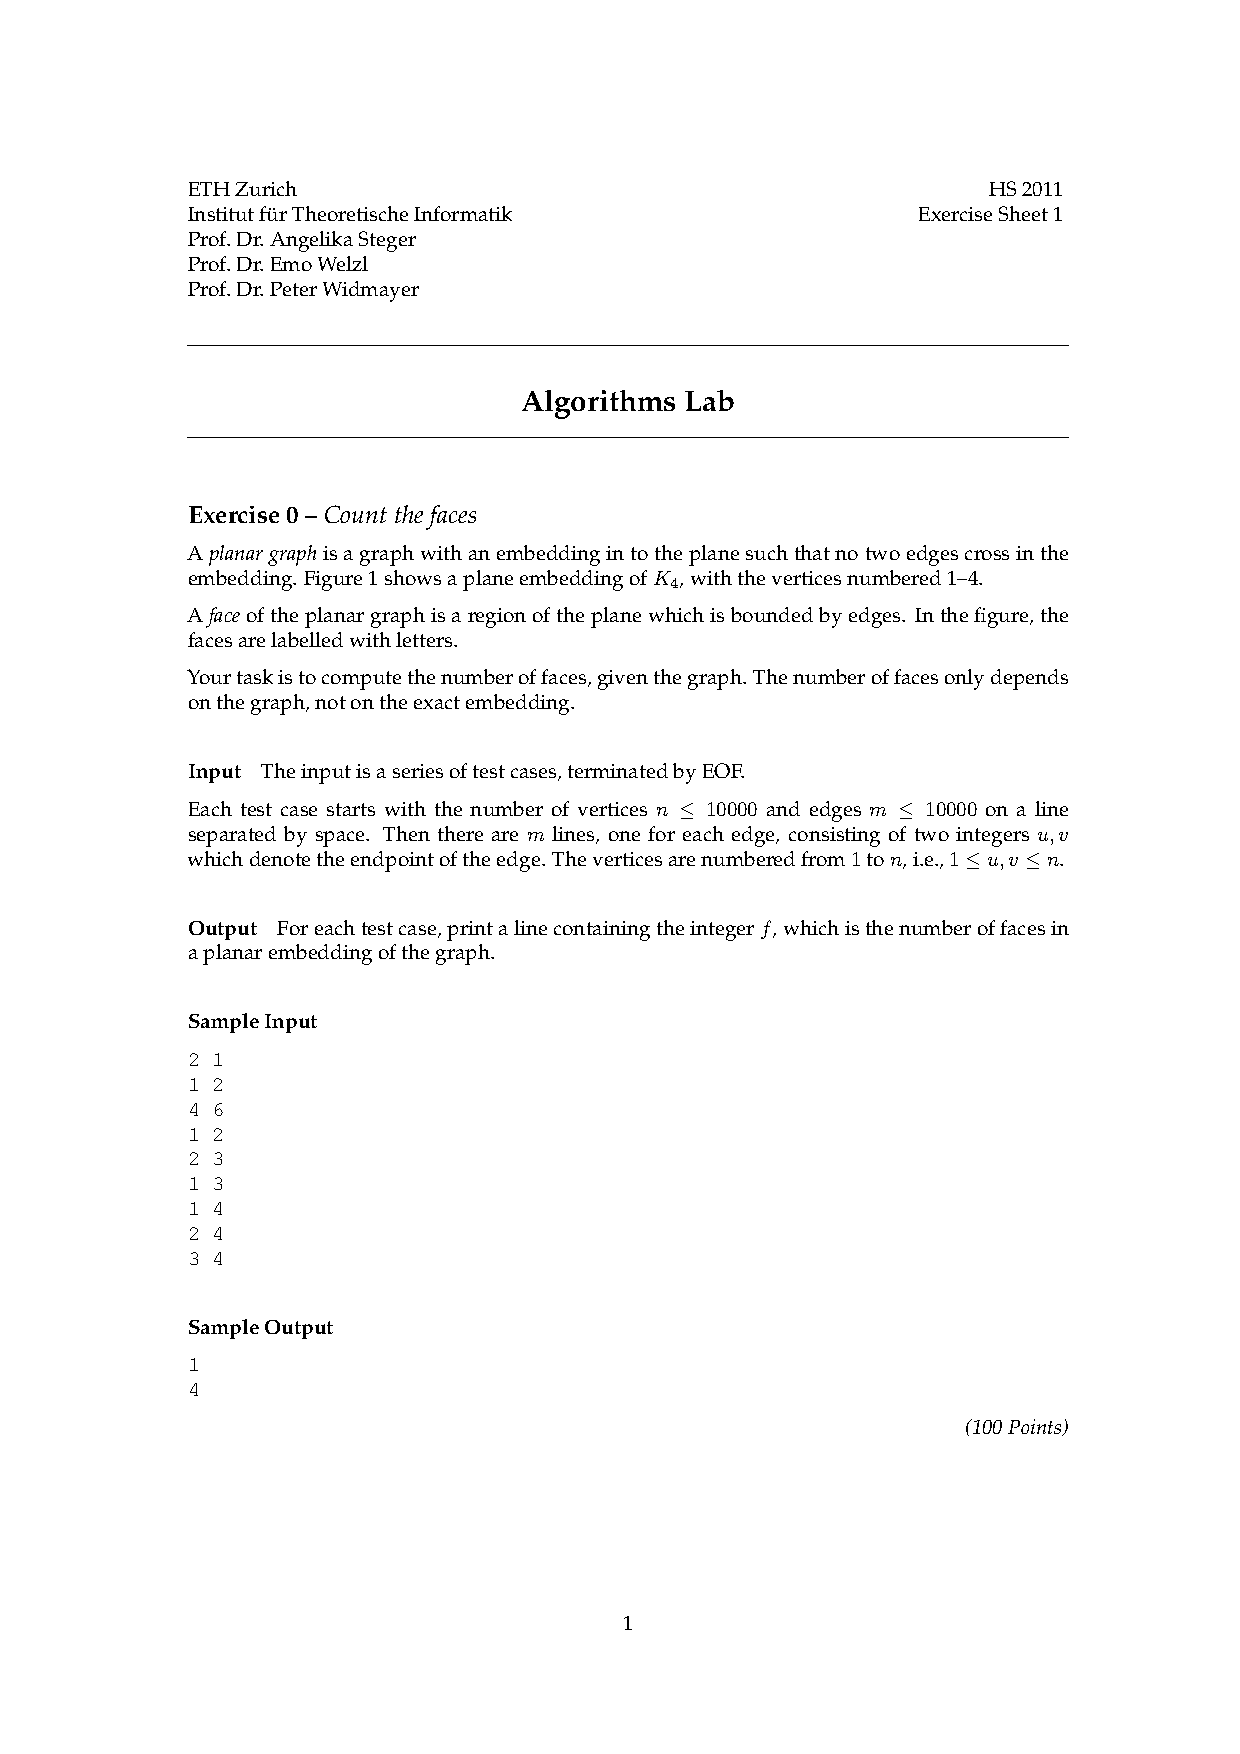
\includepdf{week_1_playground/00/countthefaces.pdf}
\lstinputlisting{week_1_playground/00/faces.cpp}

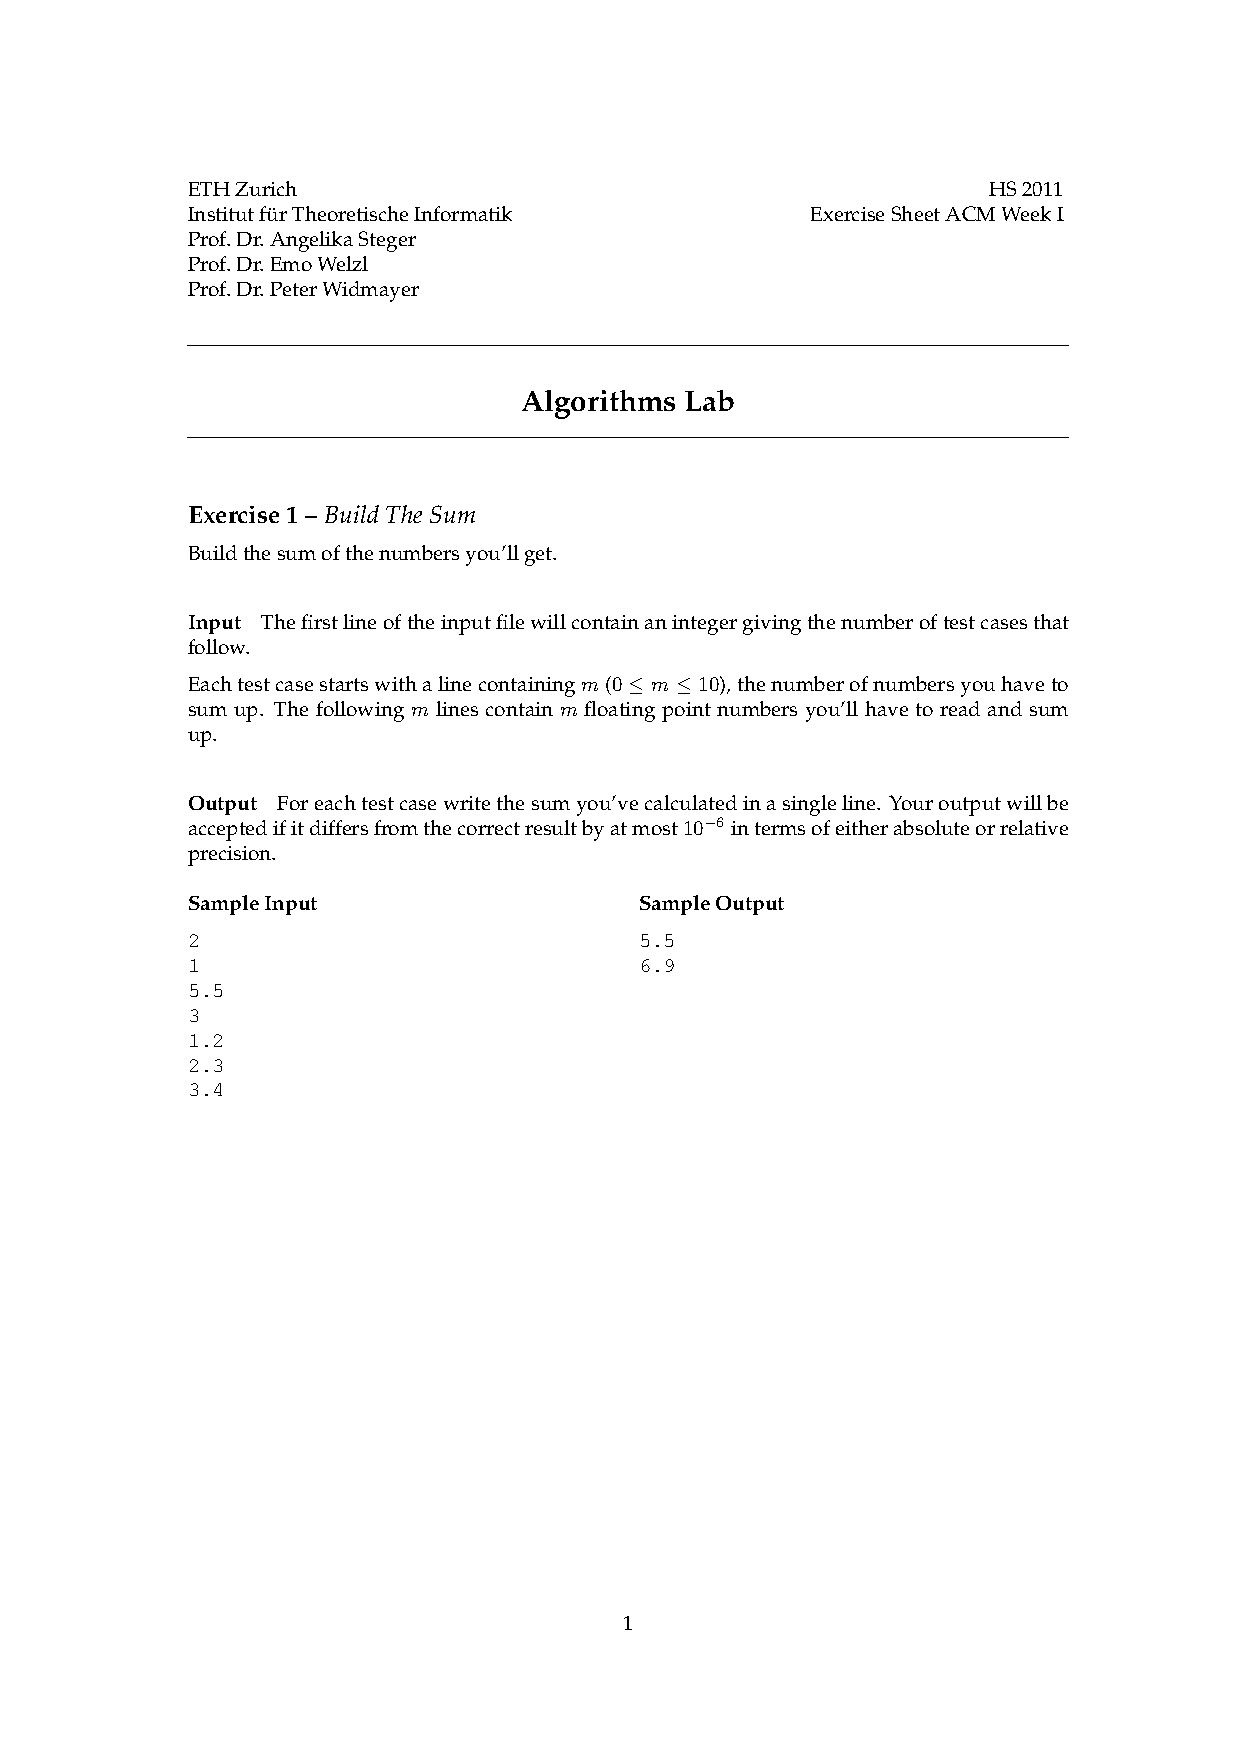
\includepdf{week_1_playground/01/BuildTheSum.pdf}
\lstinputlisting{week_1_playground/01/buildthesum.cpp}

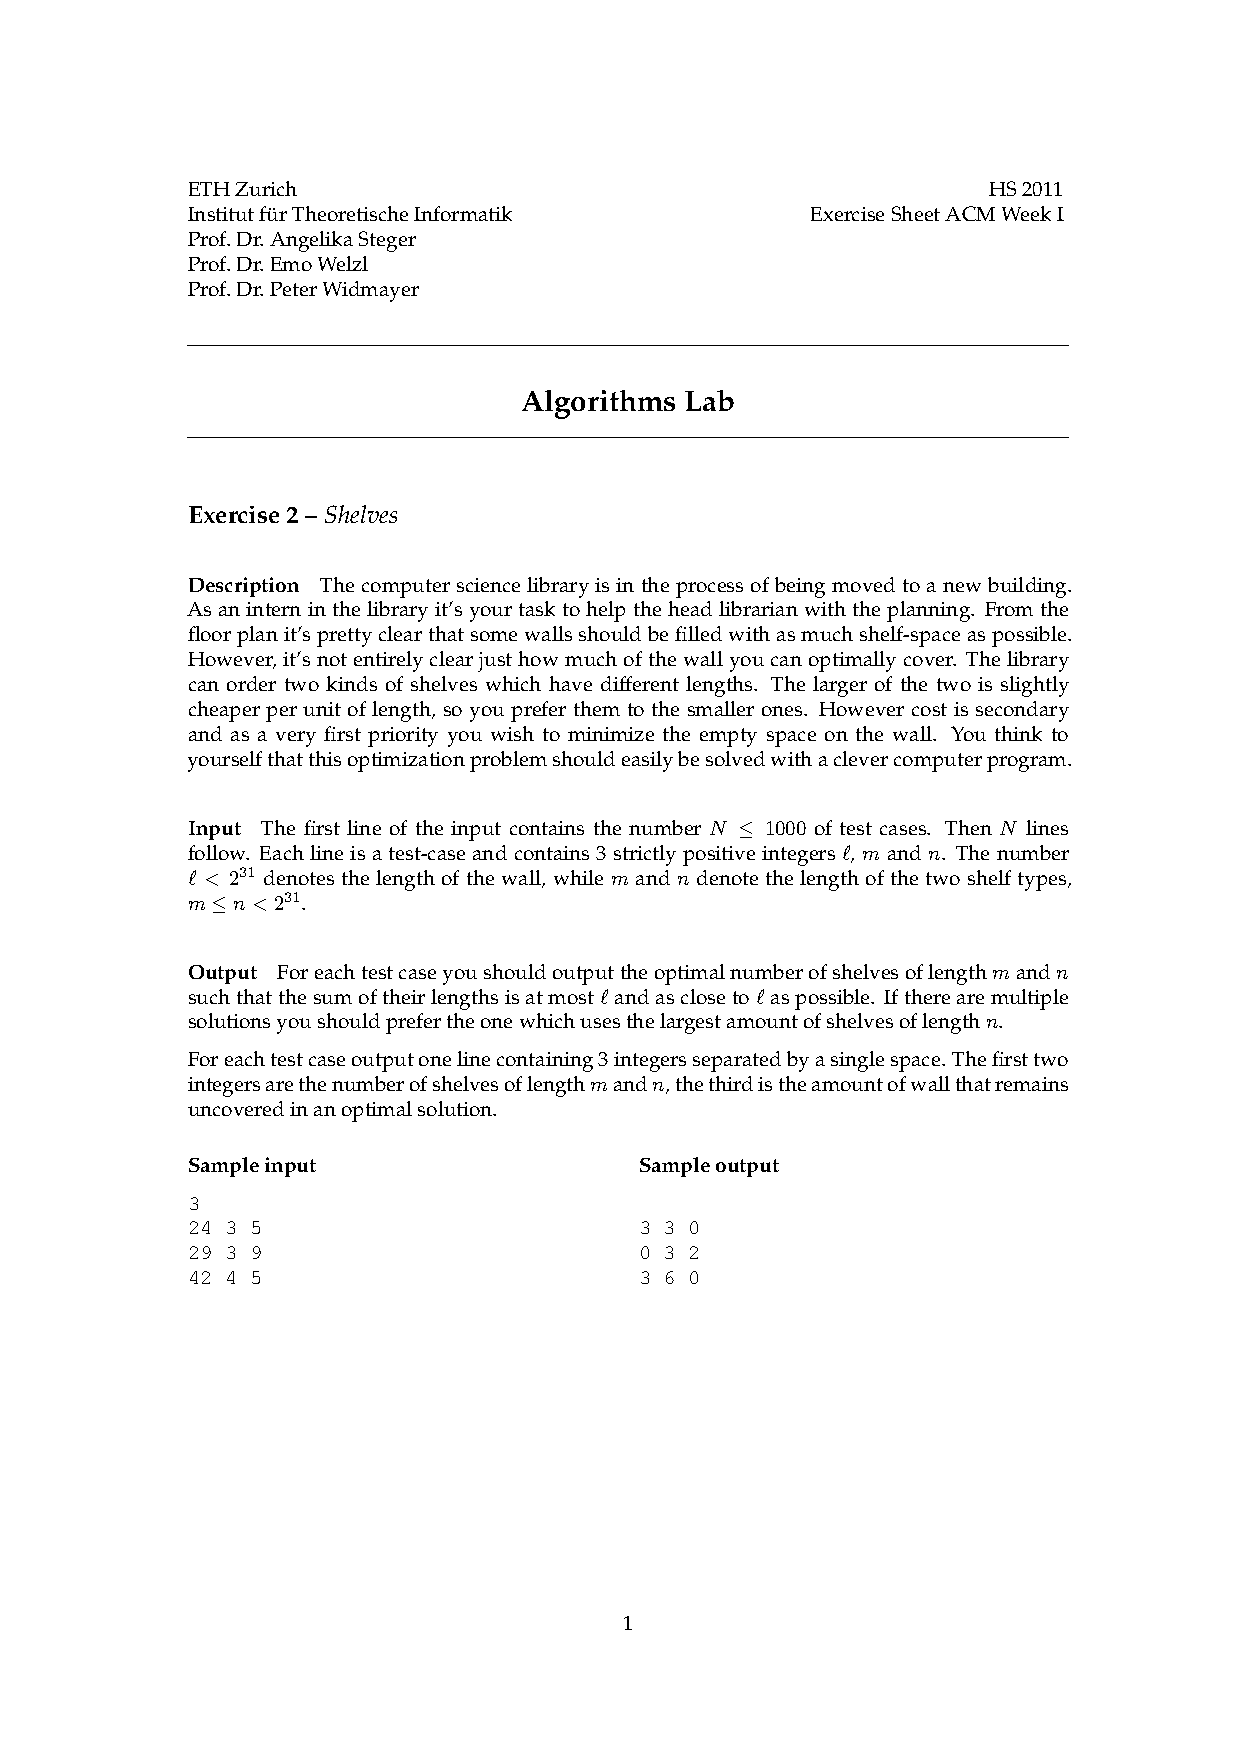
\includepdf{./week_1_playground/02/shelves.pdf}
\lstinputlisting{./week_1_playground/02/shelves.cpp}

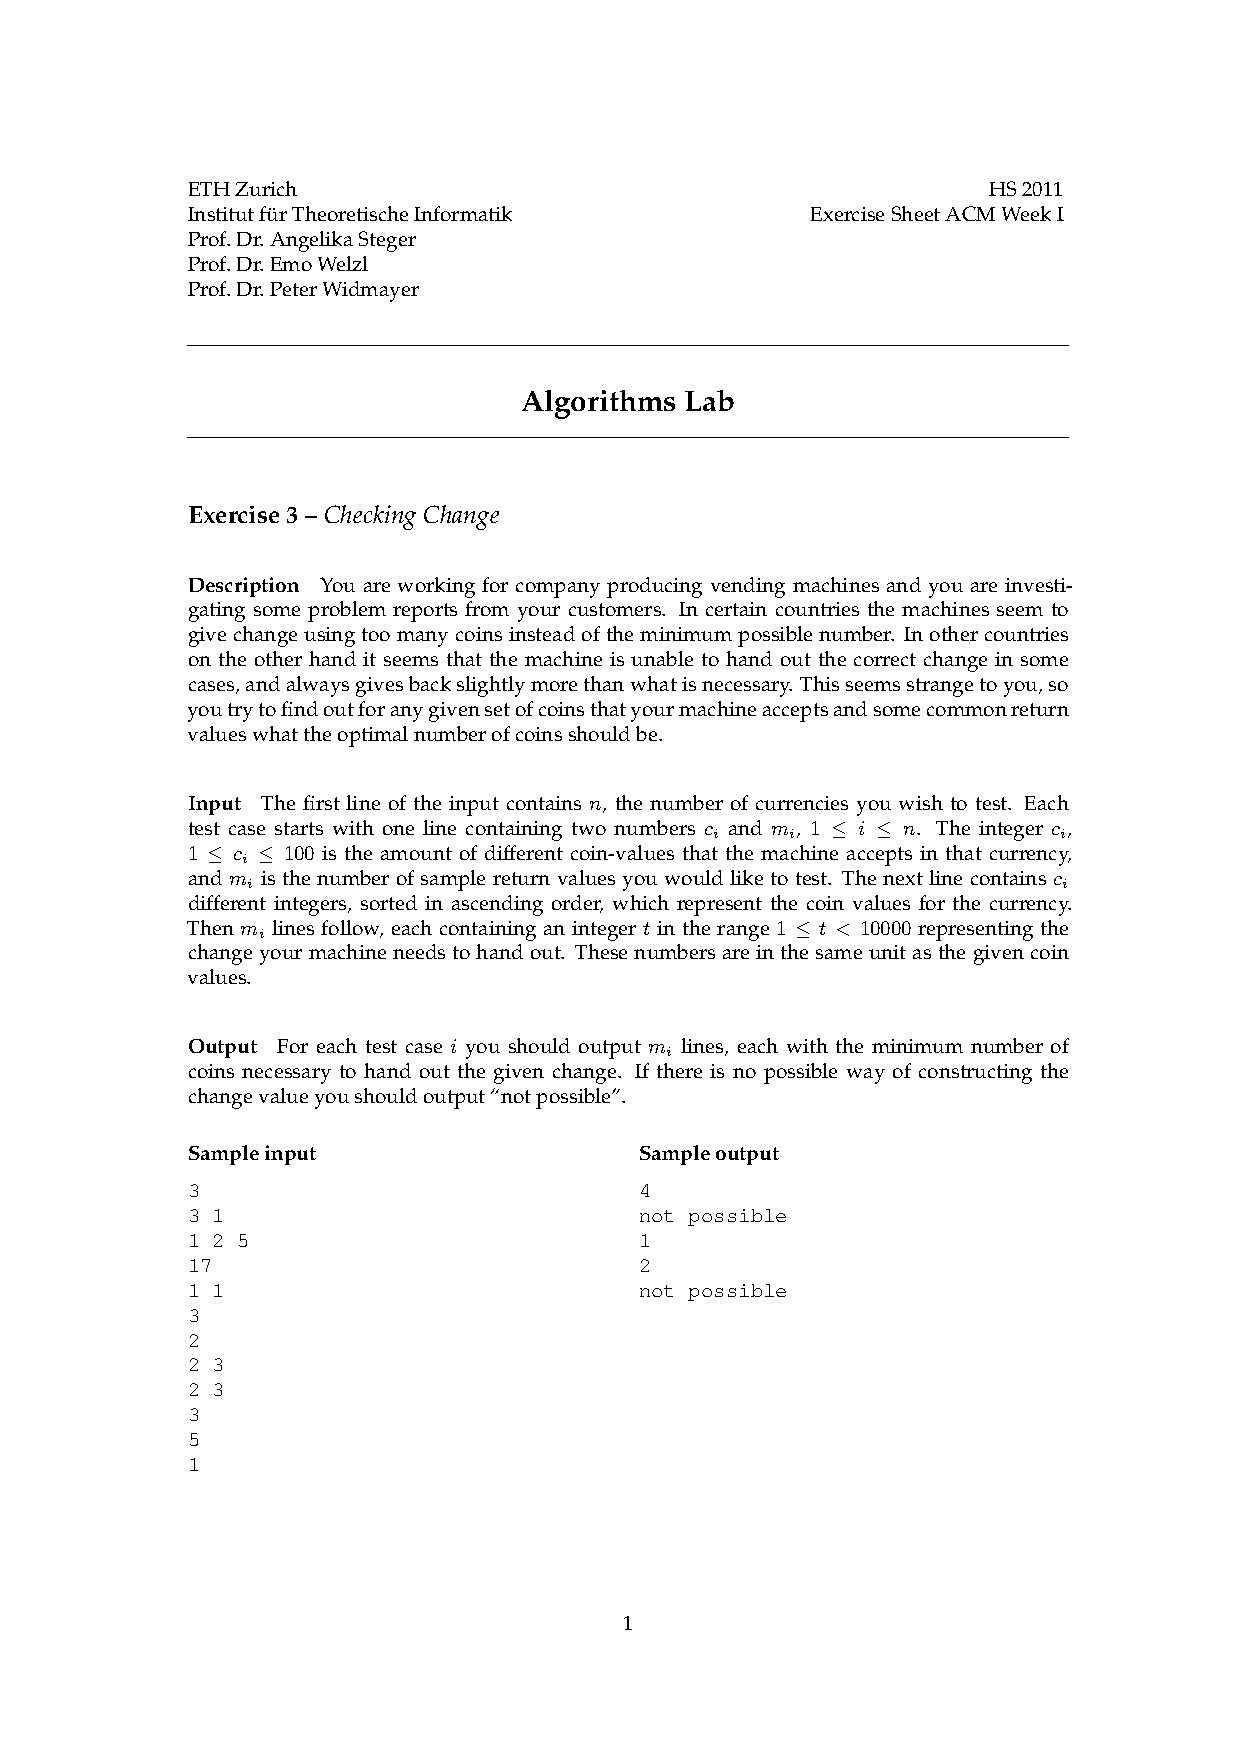
\includepdf{./week_1_playground/03/checking_change.pdf}
\lstinputlisting{./week_1_playground/03/checkingchange.cpp}

\newpage
\part{Week 2 - Playground - Part 1}
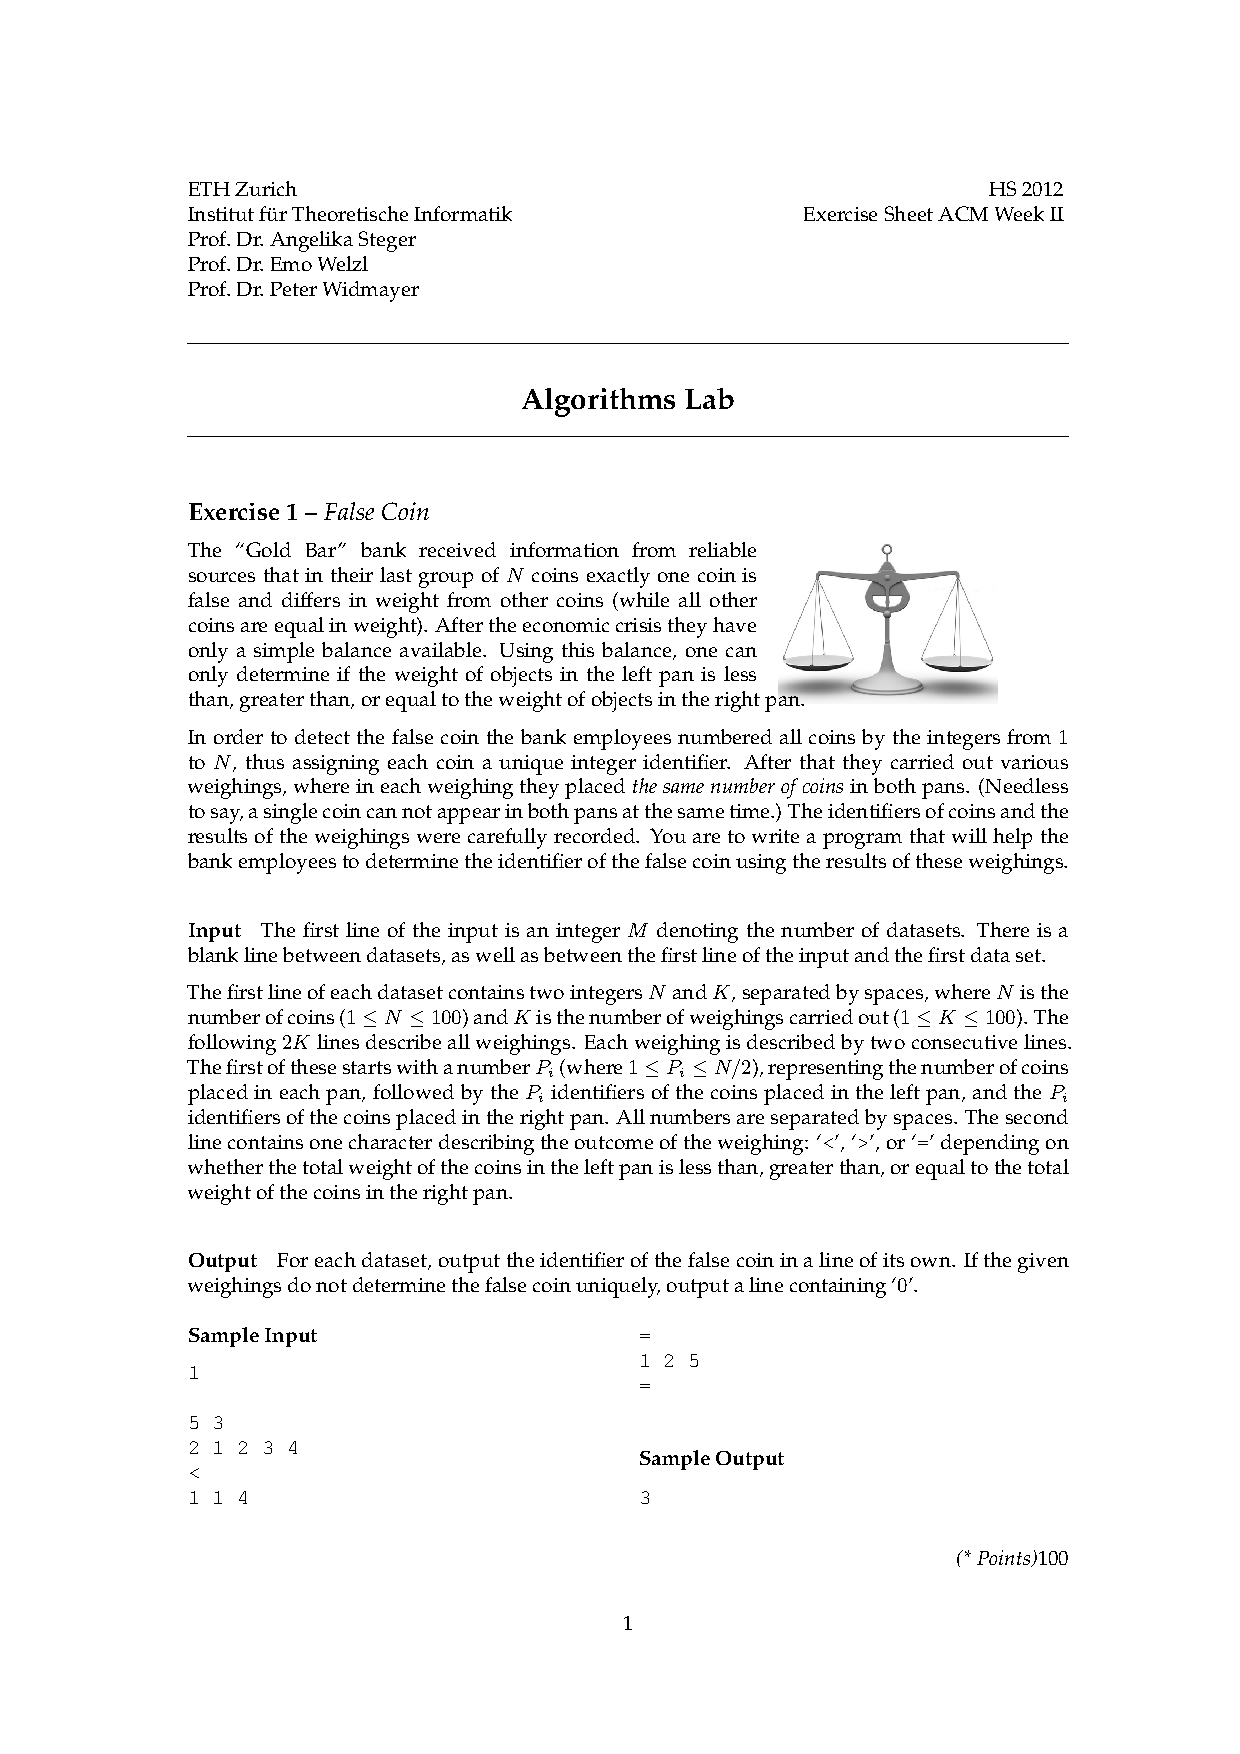
\includepdf{./week_2_fundamental/00/falsecoin.pdf}
\lstinputlisting{./week_2_fundamental/00/coins.cpp}
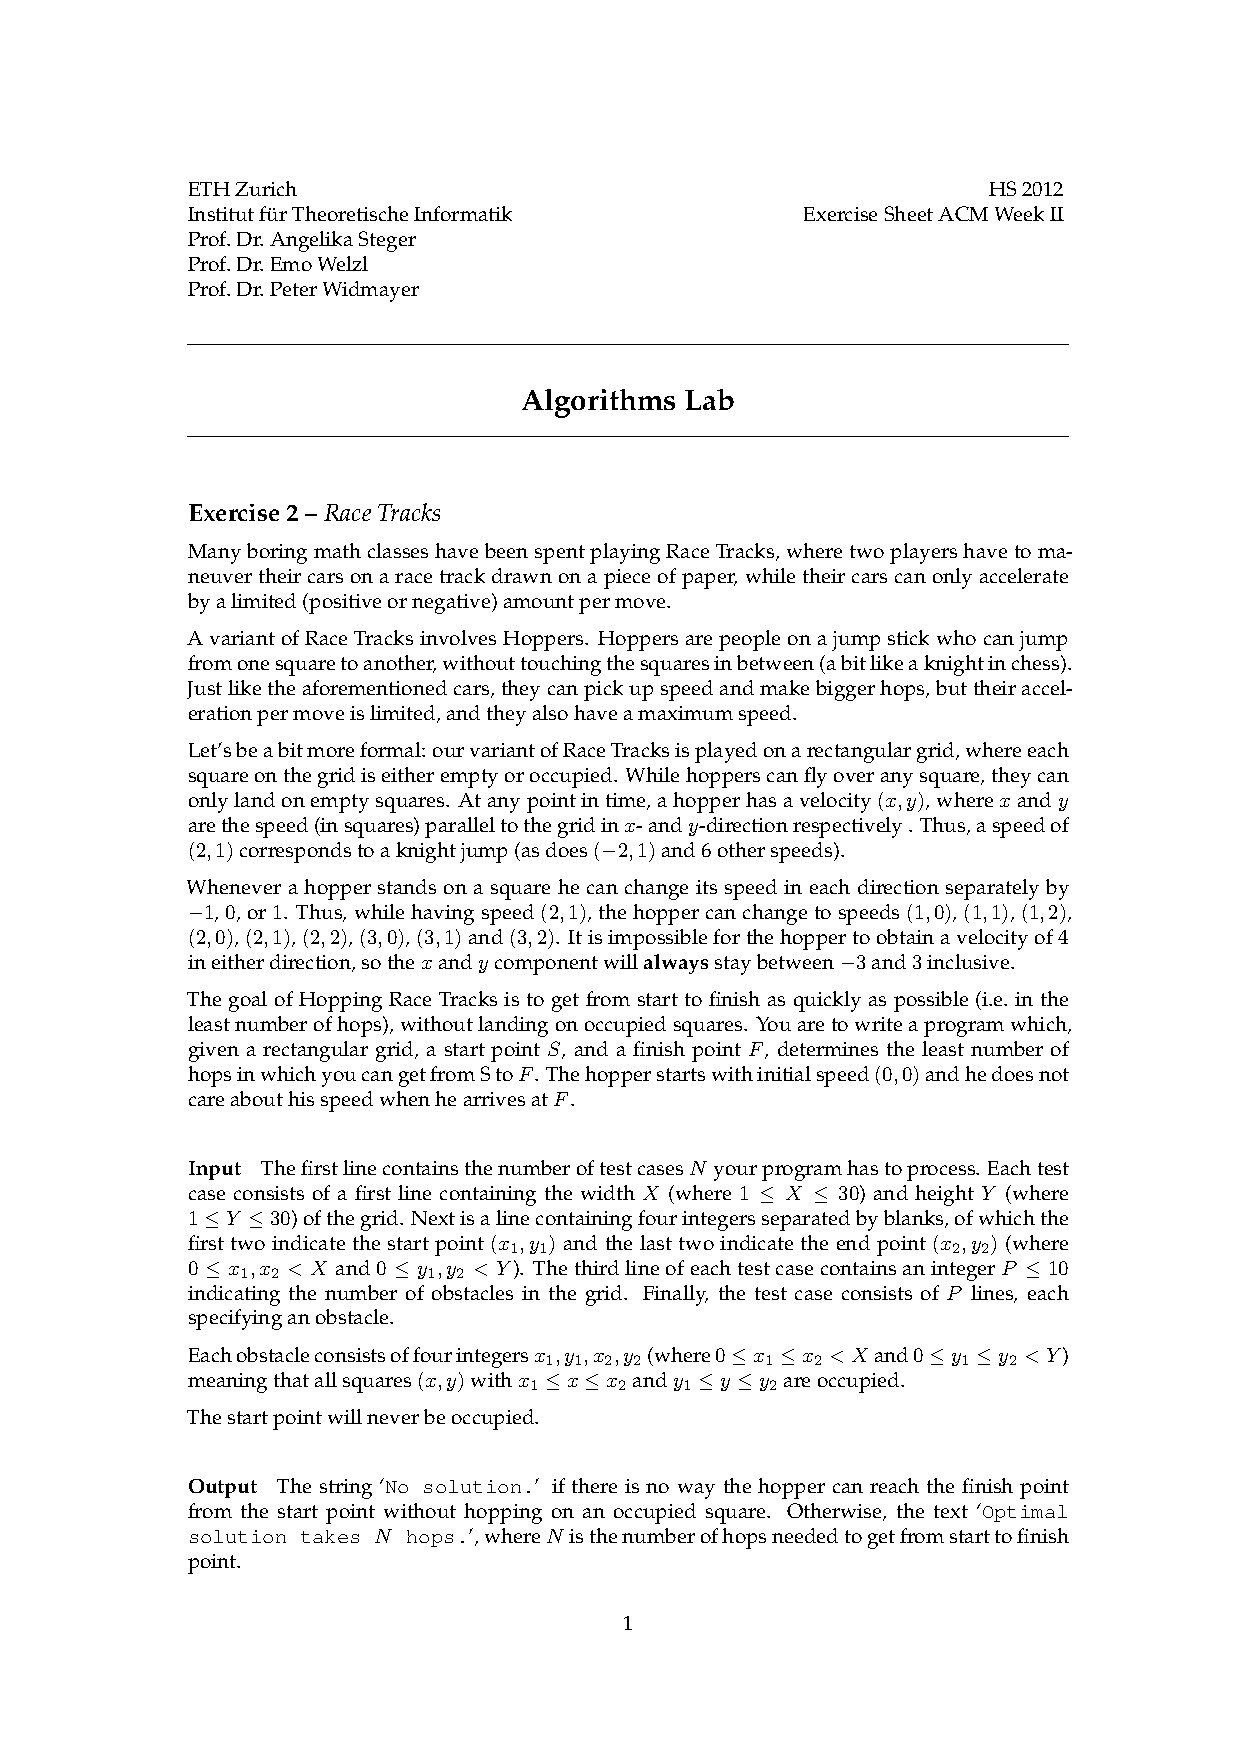
\includepdf{./week_2_fundamental/01/race_tracks.pdf}
\lstinputlisting{./week_2_fundamental/01/tracks.cpp}
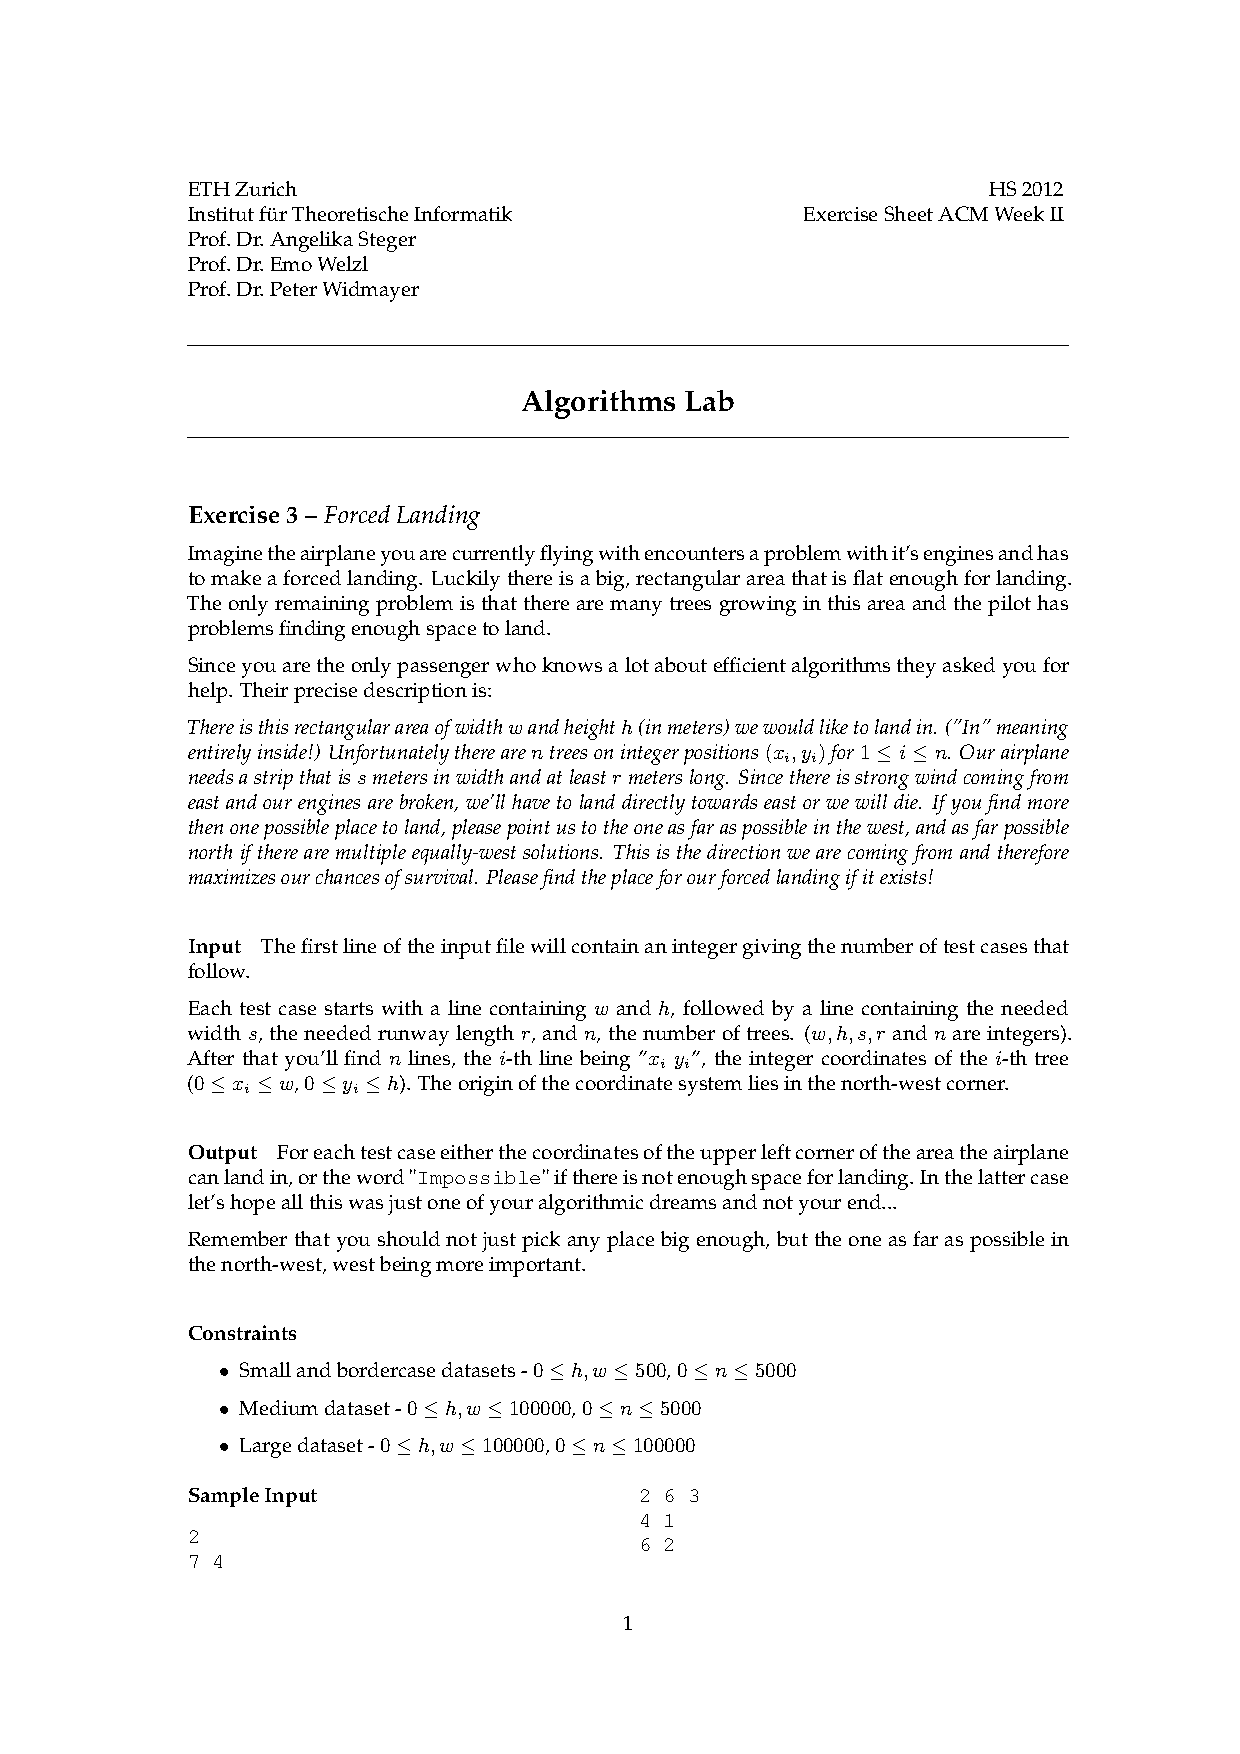
\includepdf{./week_2_fundamental/02/ForcedLanding.pdf}
Warning: Solution broken
\lstinputlisting{./week_2_fundamental/02/landing4.cpp}
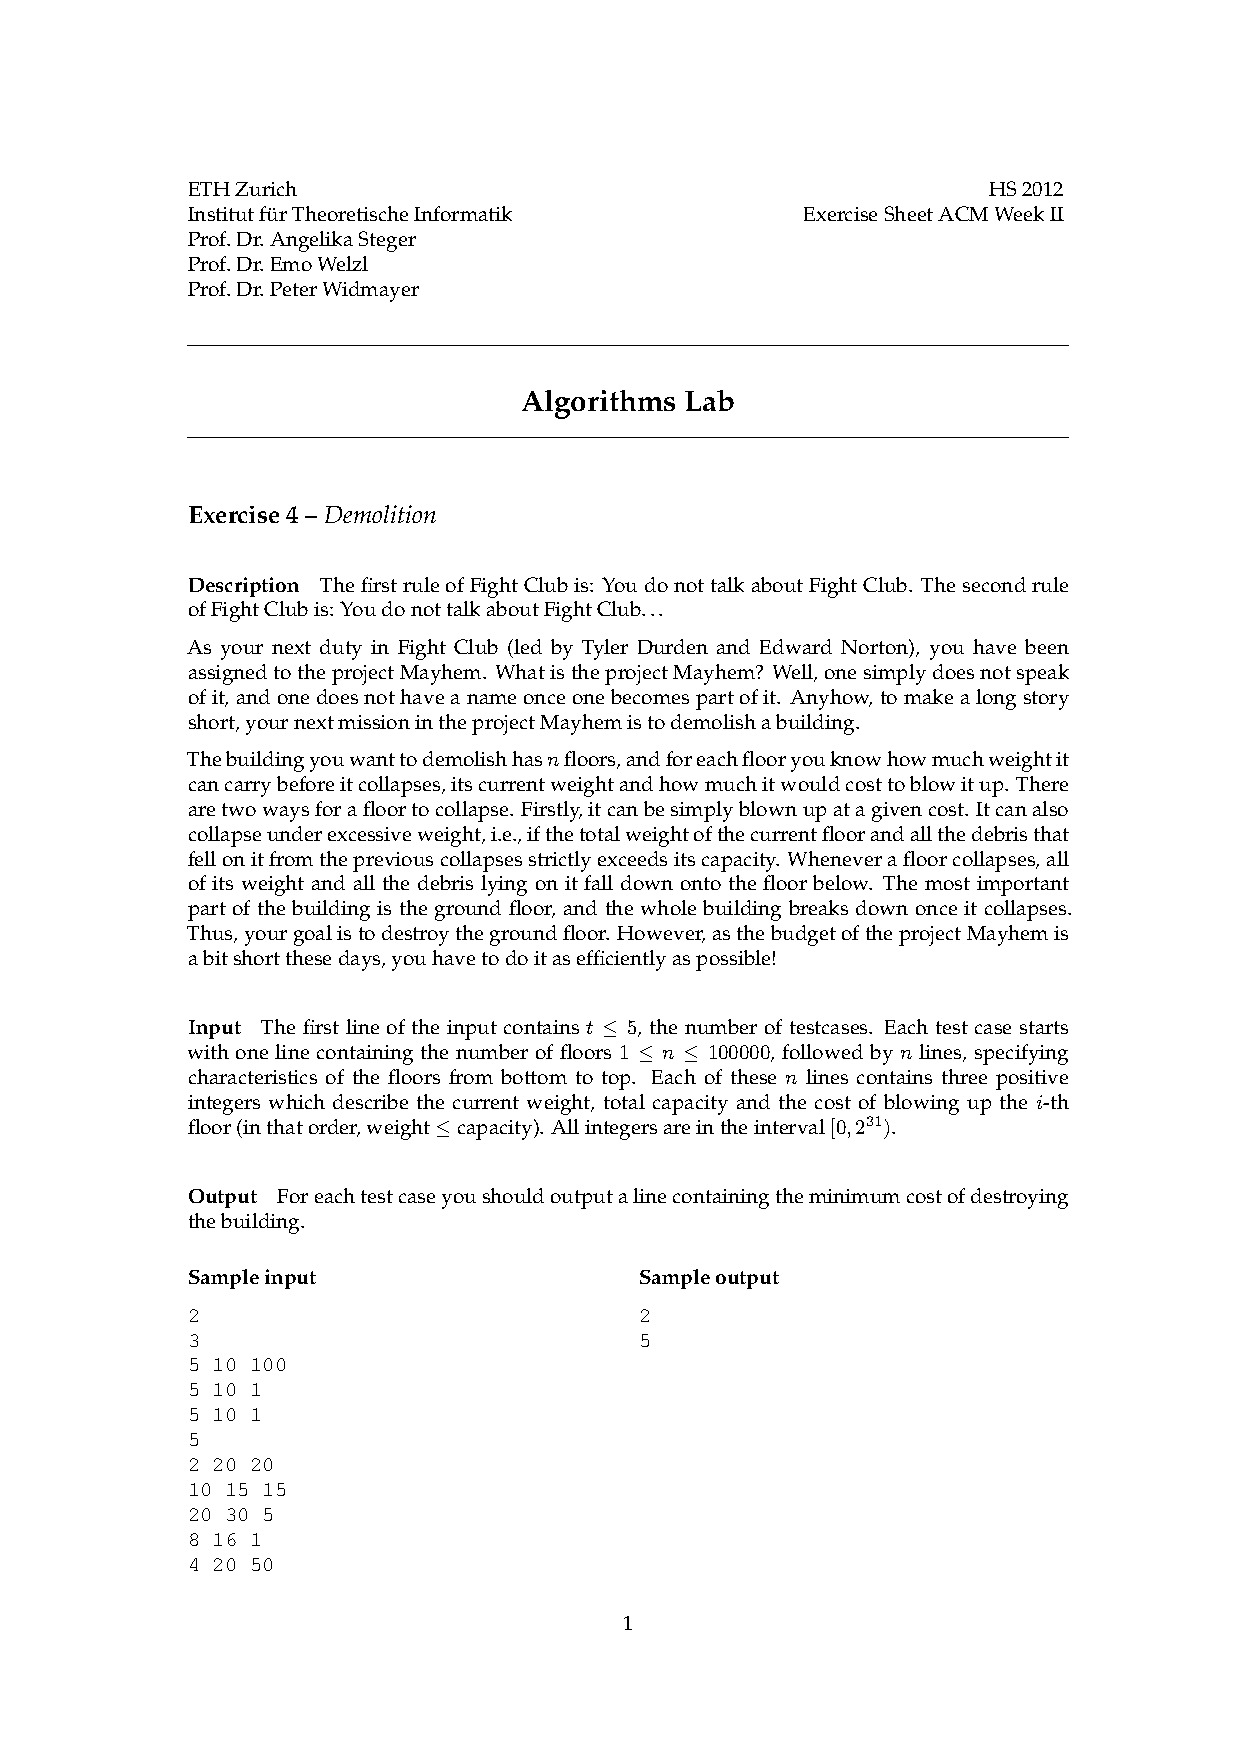
\includepdf{./week_2_fundamental/03/demolition.pdf}
Warning: Solution broken
\lstinputlisting{./week_2_fundamental/03/demolition.cpp}

\newpage
\part{Week 3 - Playground - Part 2}
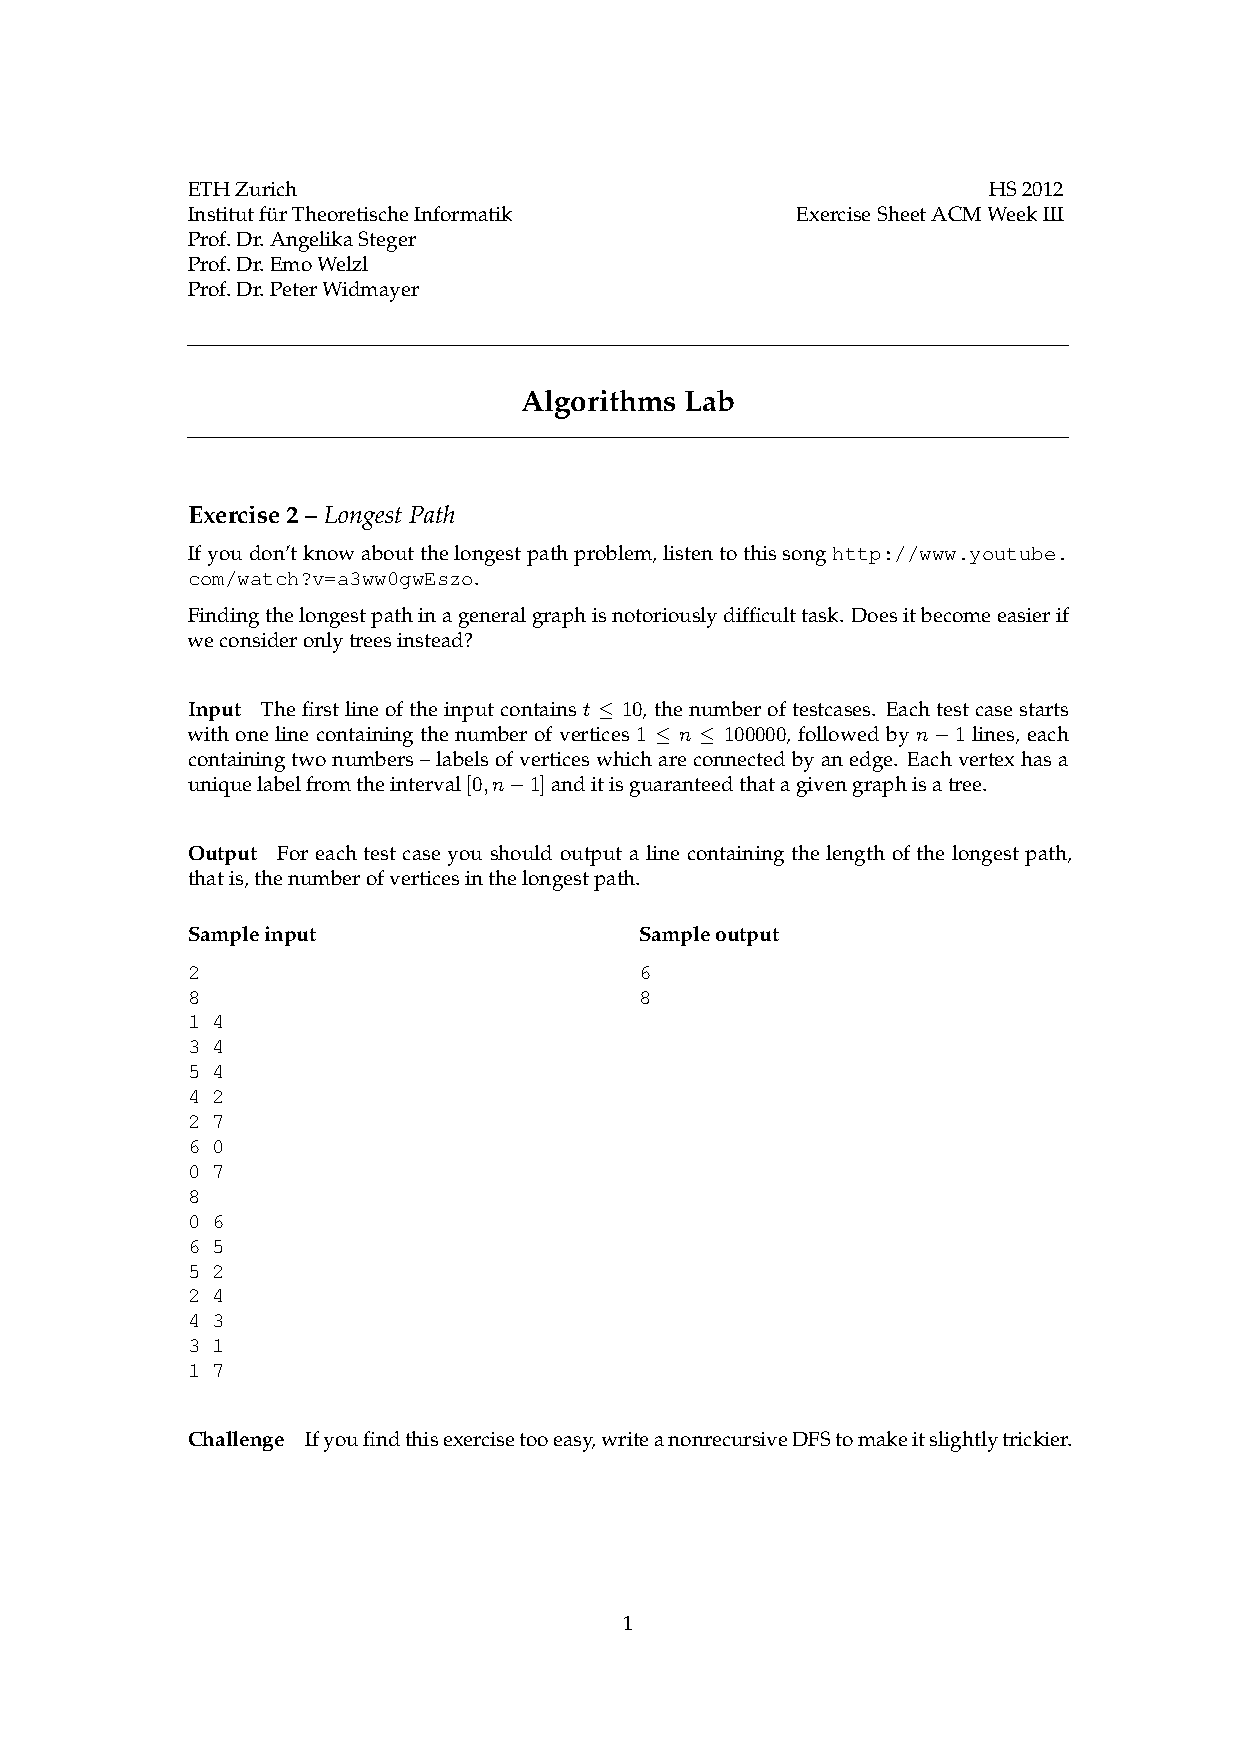
\includepdf{./week_3_fundamental_2/00/longestpath.pdf}
\lstinputlisting{./week_3_fundamental_2/00/longest_path/main.cpp}
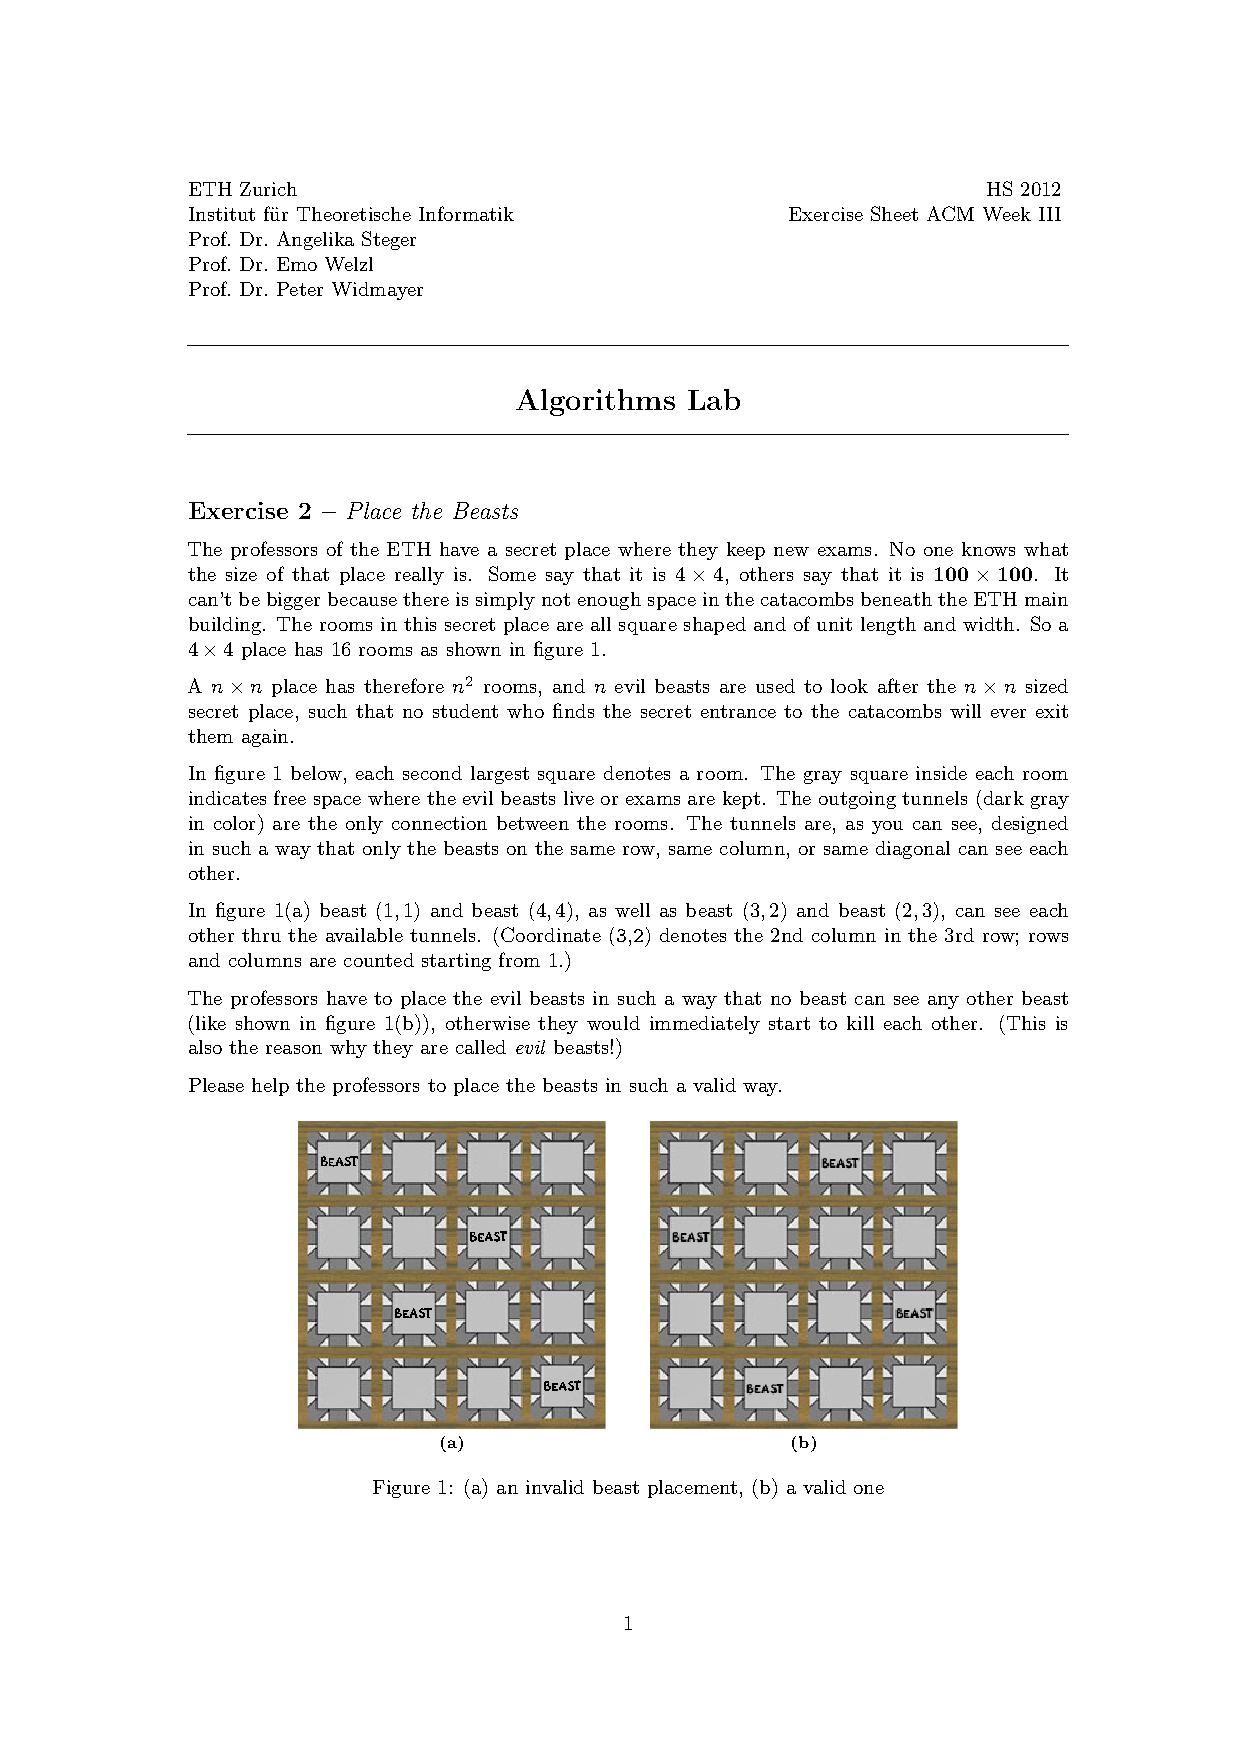
\includepdf{./week_3_fundamental_2/01/beasts.pdf}
\lstinputlisting{./week_3_fundamental_2/01/beasts/main.cpp}
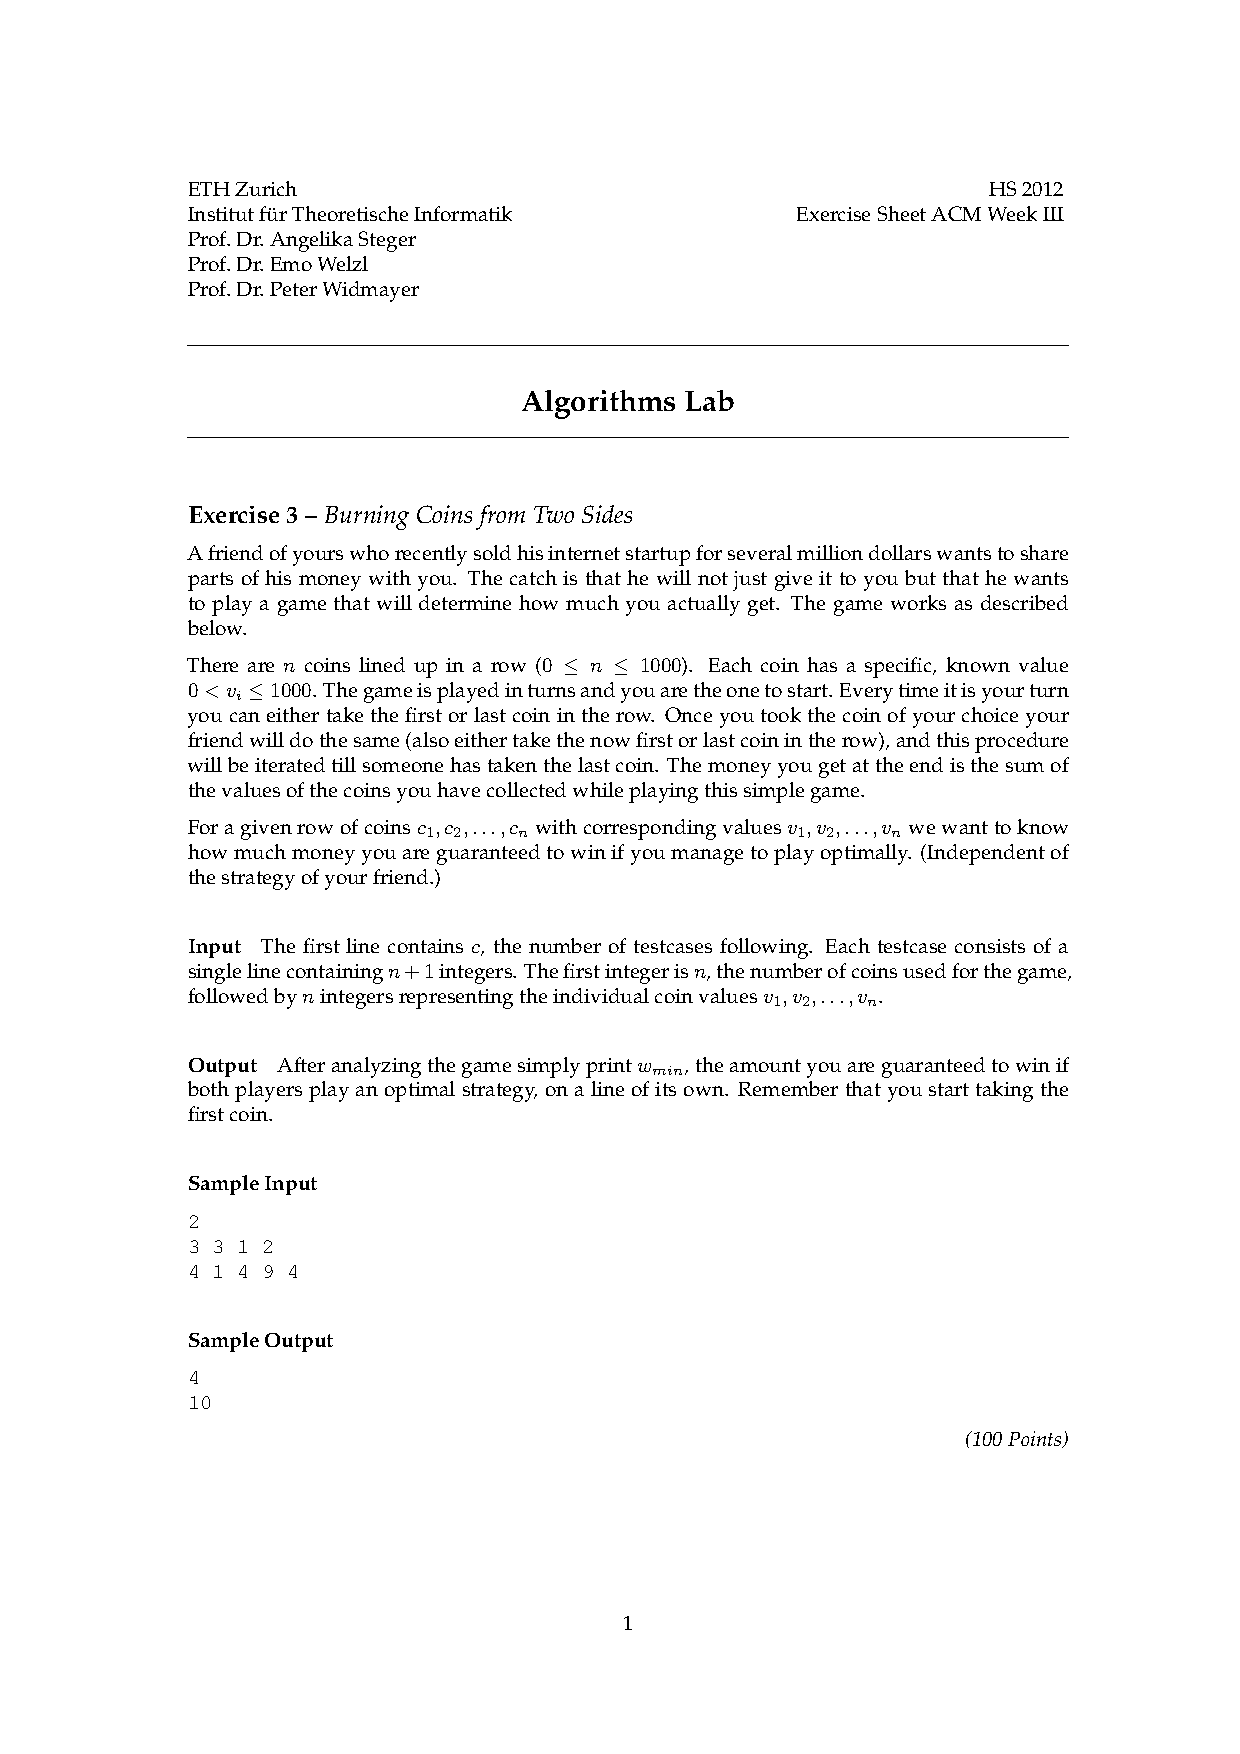
\includepdf{./week_3_fundamental_2/02/burningcoins.pdf}
\lstinputlisting{./week_3_fundamental_2/02/burningcoins/main.cpp}
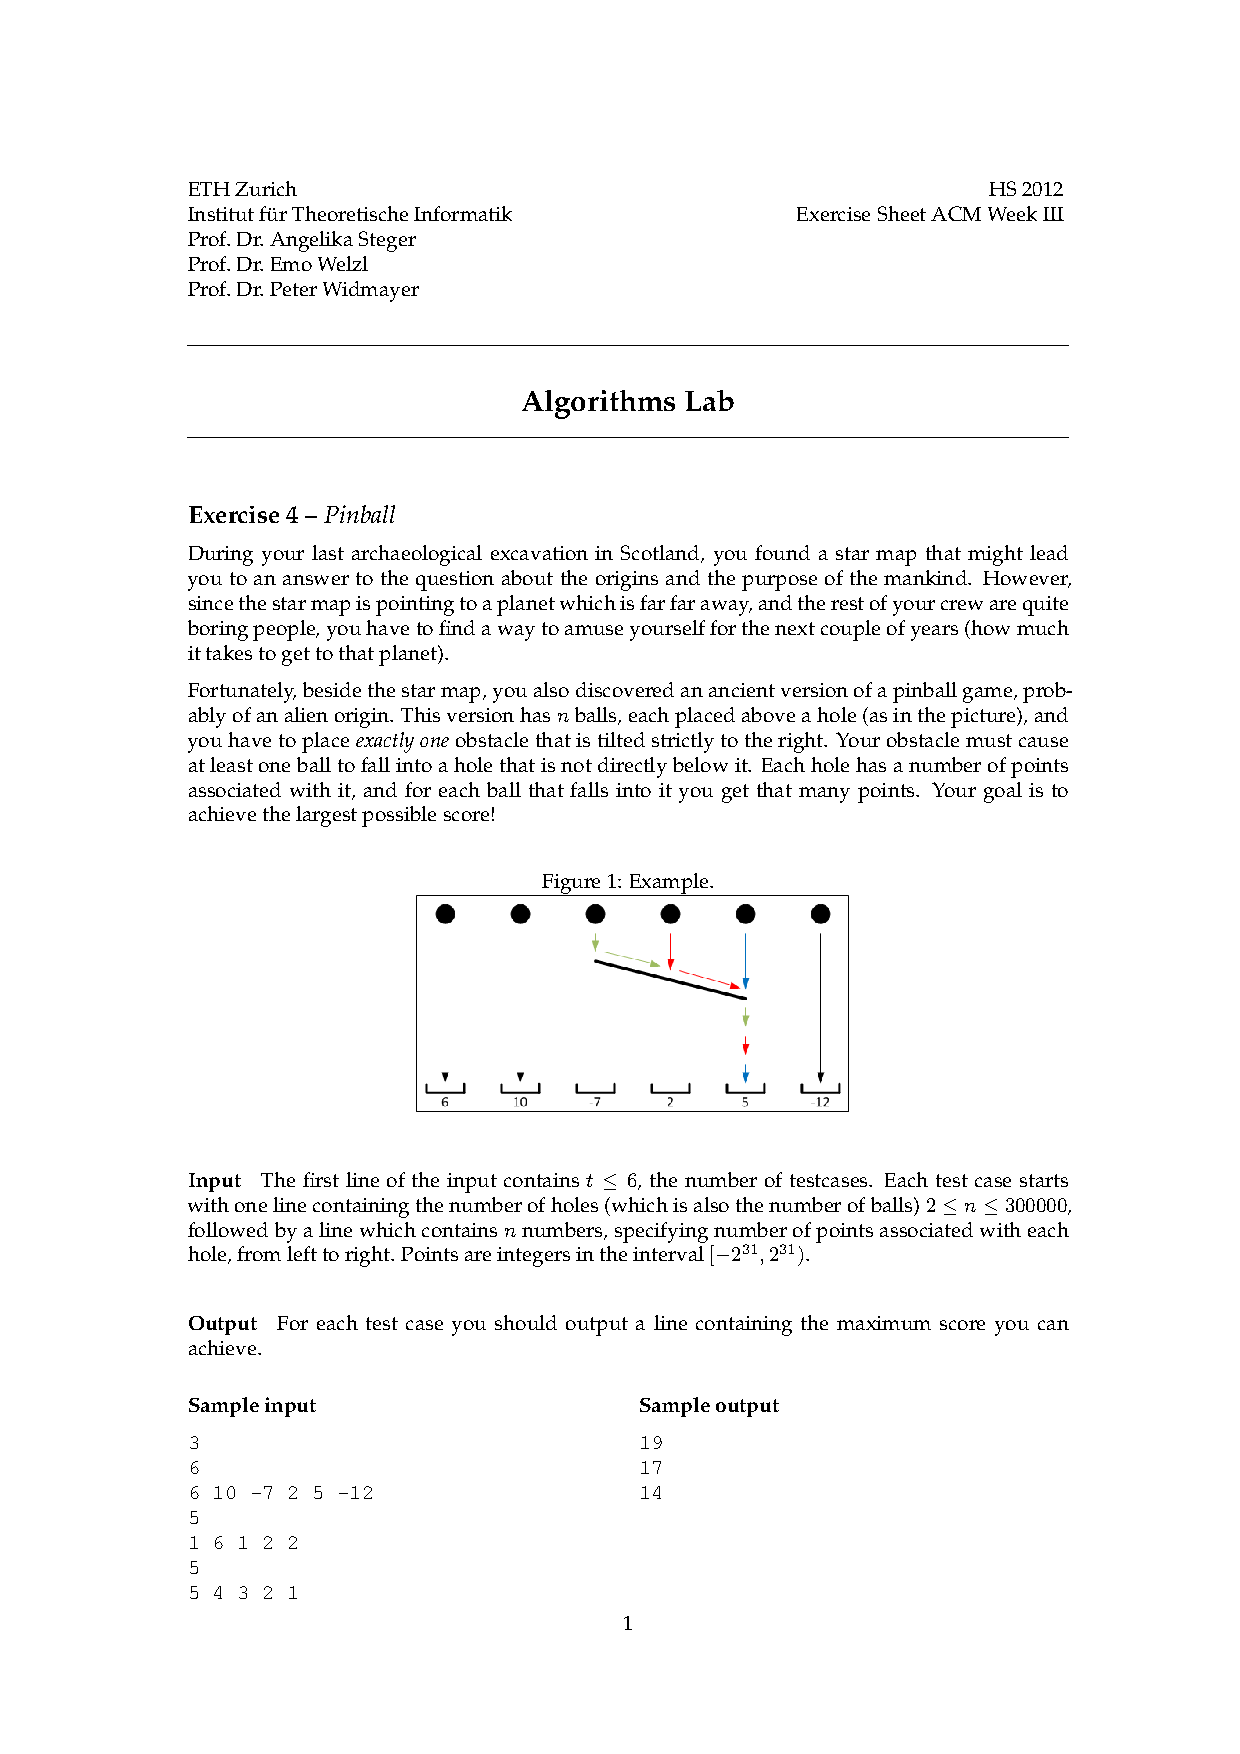
\includepdf{./week_3_fundamental_2/03/pinball.pdf}
\lstinputlisting{./week_3_fundamental_2/03/pinball/main.cpp}

\newpage
\part{Week 4 - BGL Introduction}
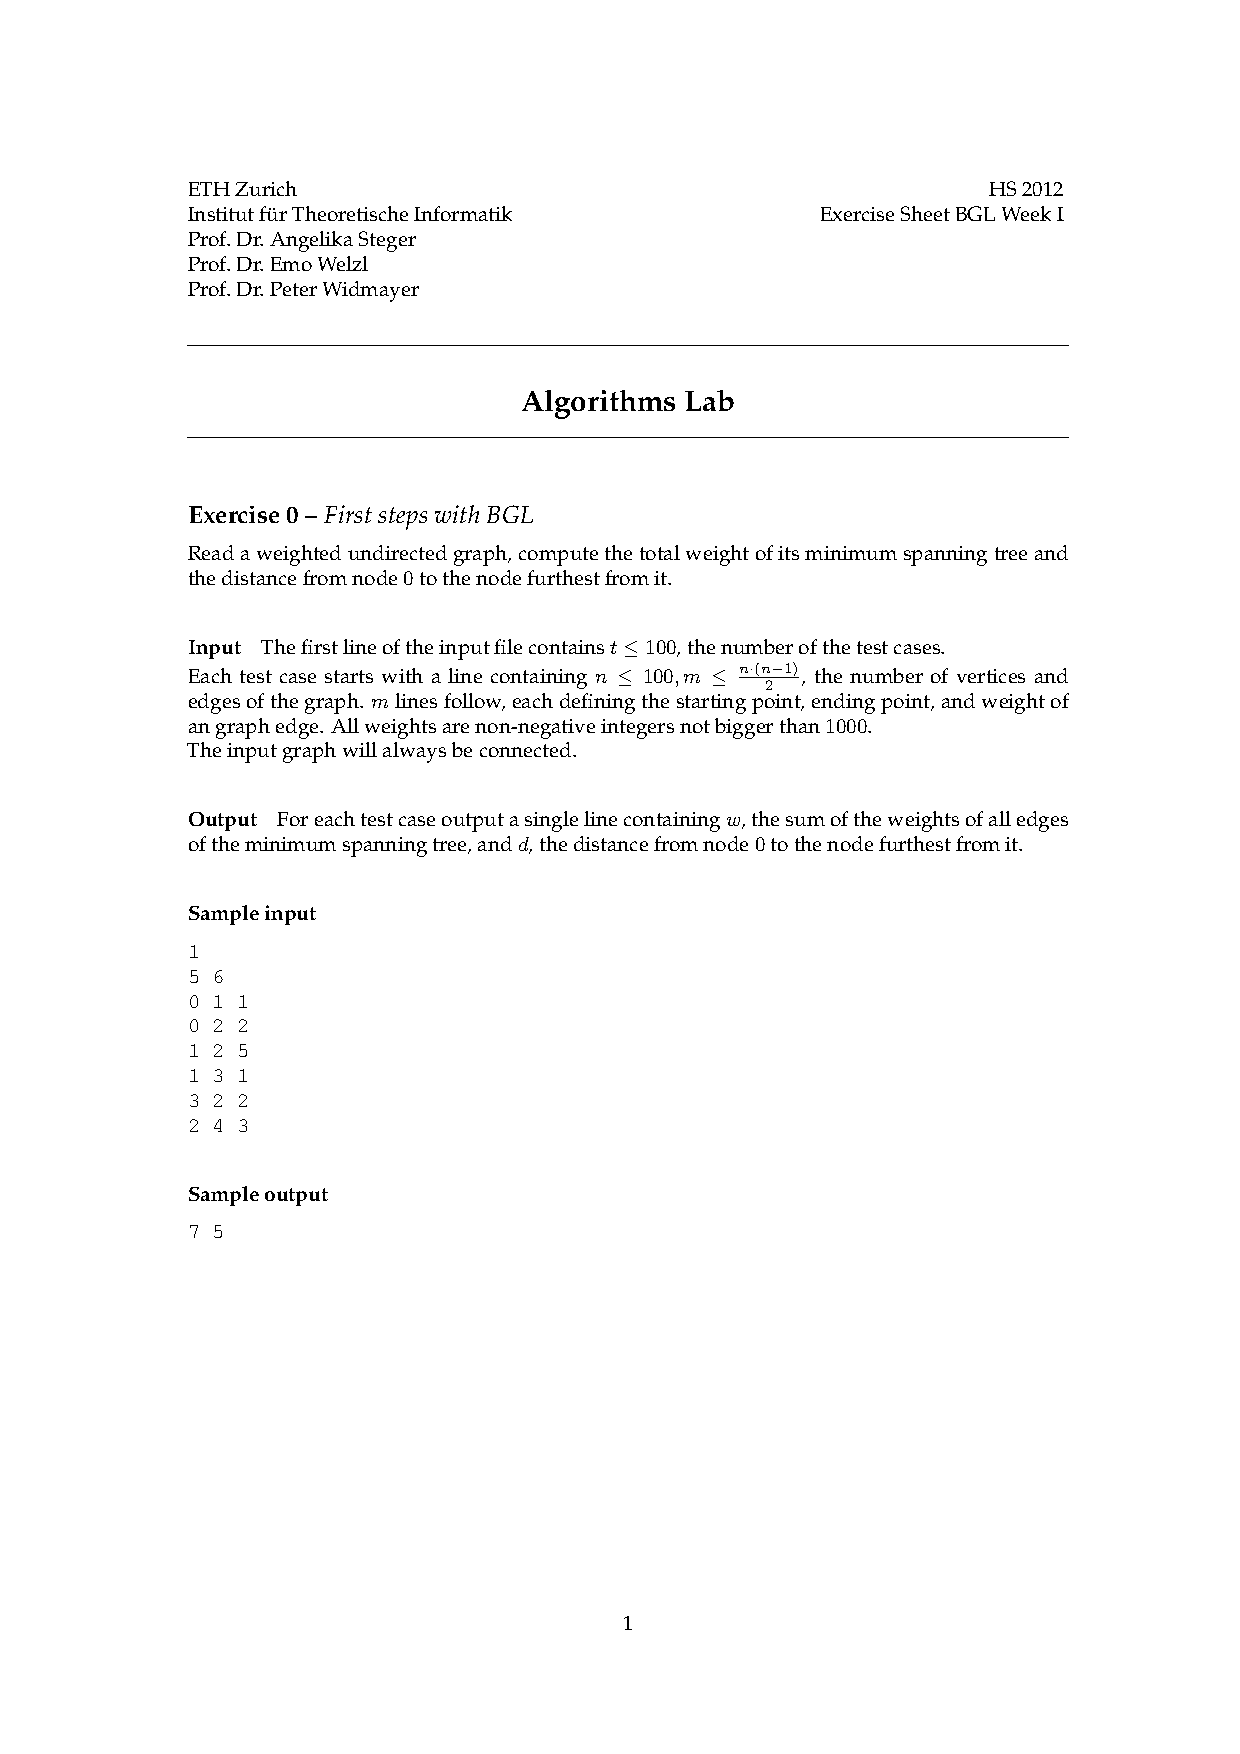
\includepdf{./week_4_bgl_introduction/0_graphs/graphs.pdf}
\lstinputlisting{./week_4_bgl_introduction/0_graphs/main.cpp}
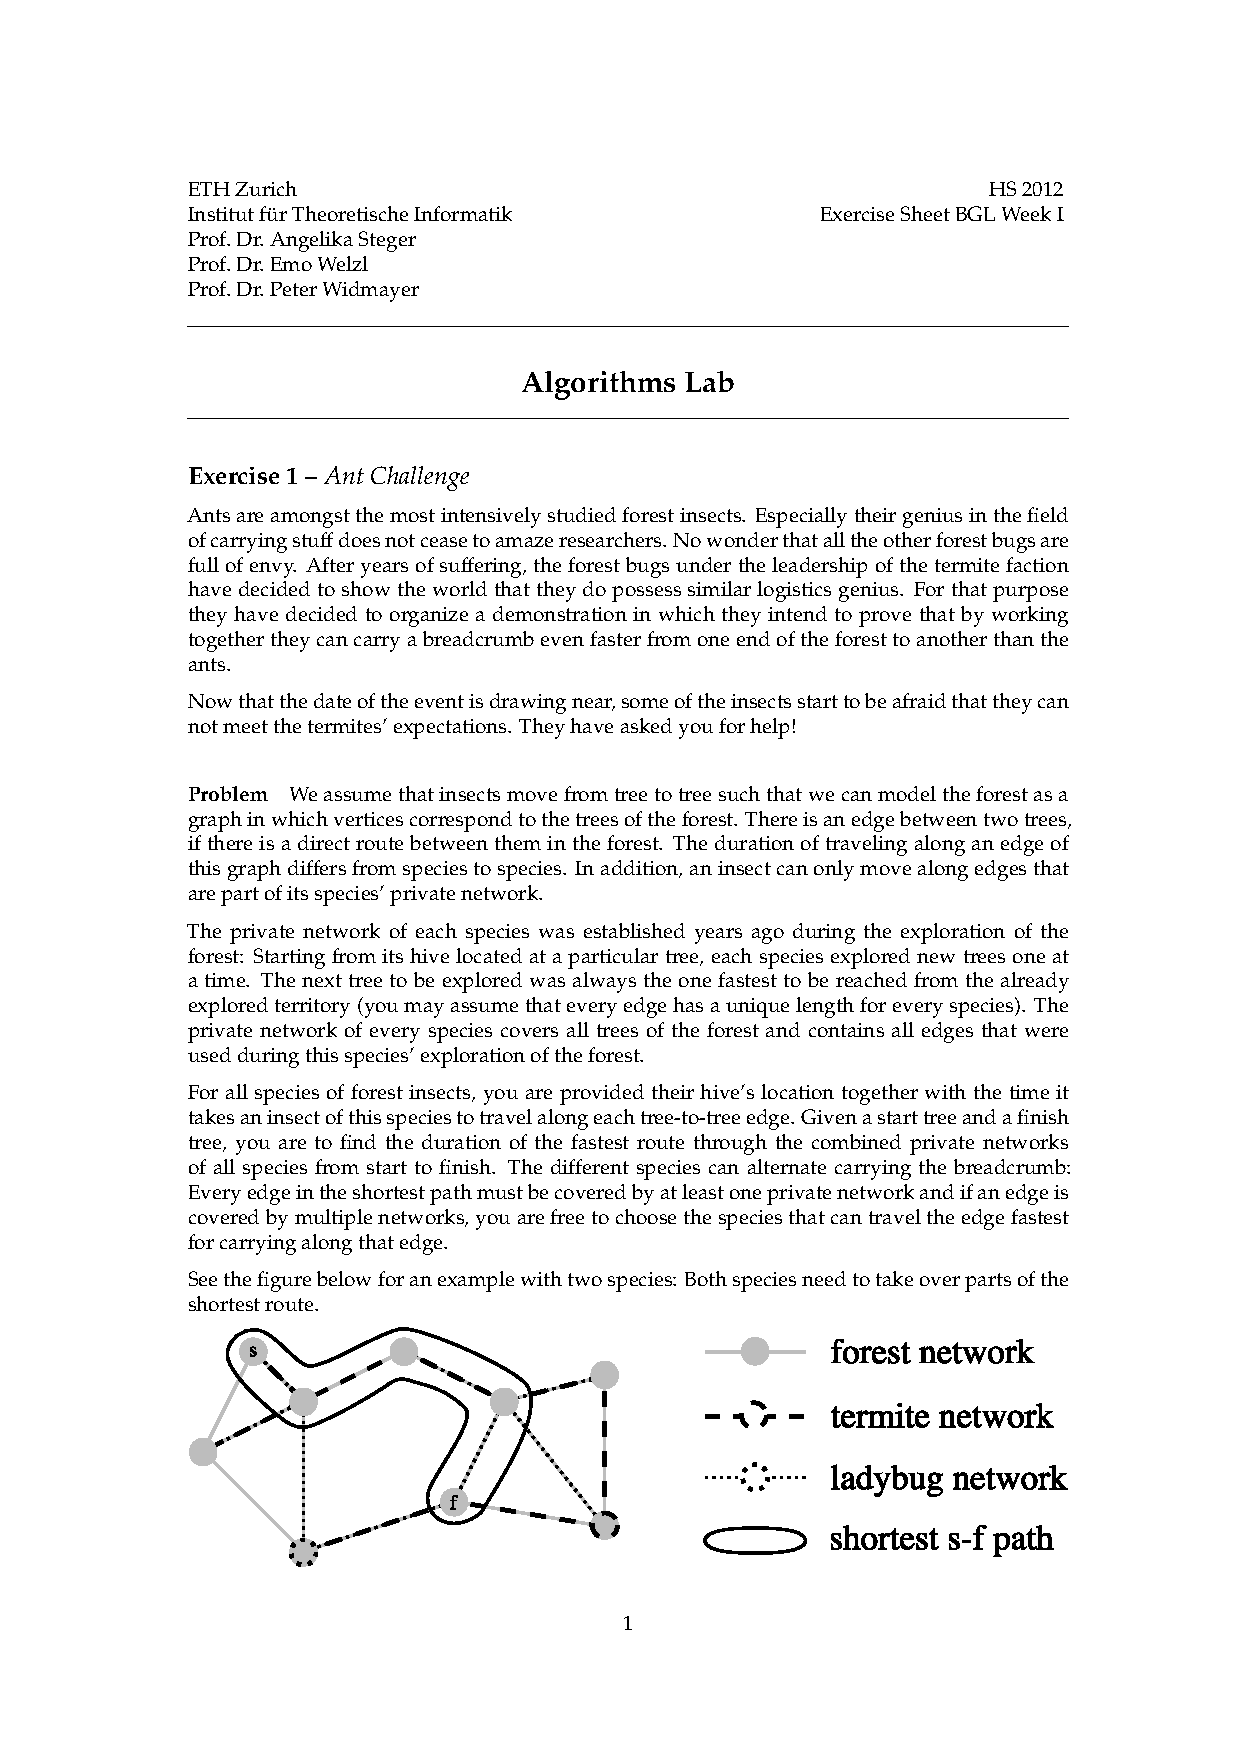
\includepdf{./week_4_bgl_introduction/1_ant_challenge/ant_challenge.pdf}
\lstinputlisting{./week_4_bgl_introduction/1_ant_challenge/main.cpp}
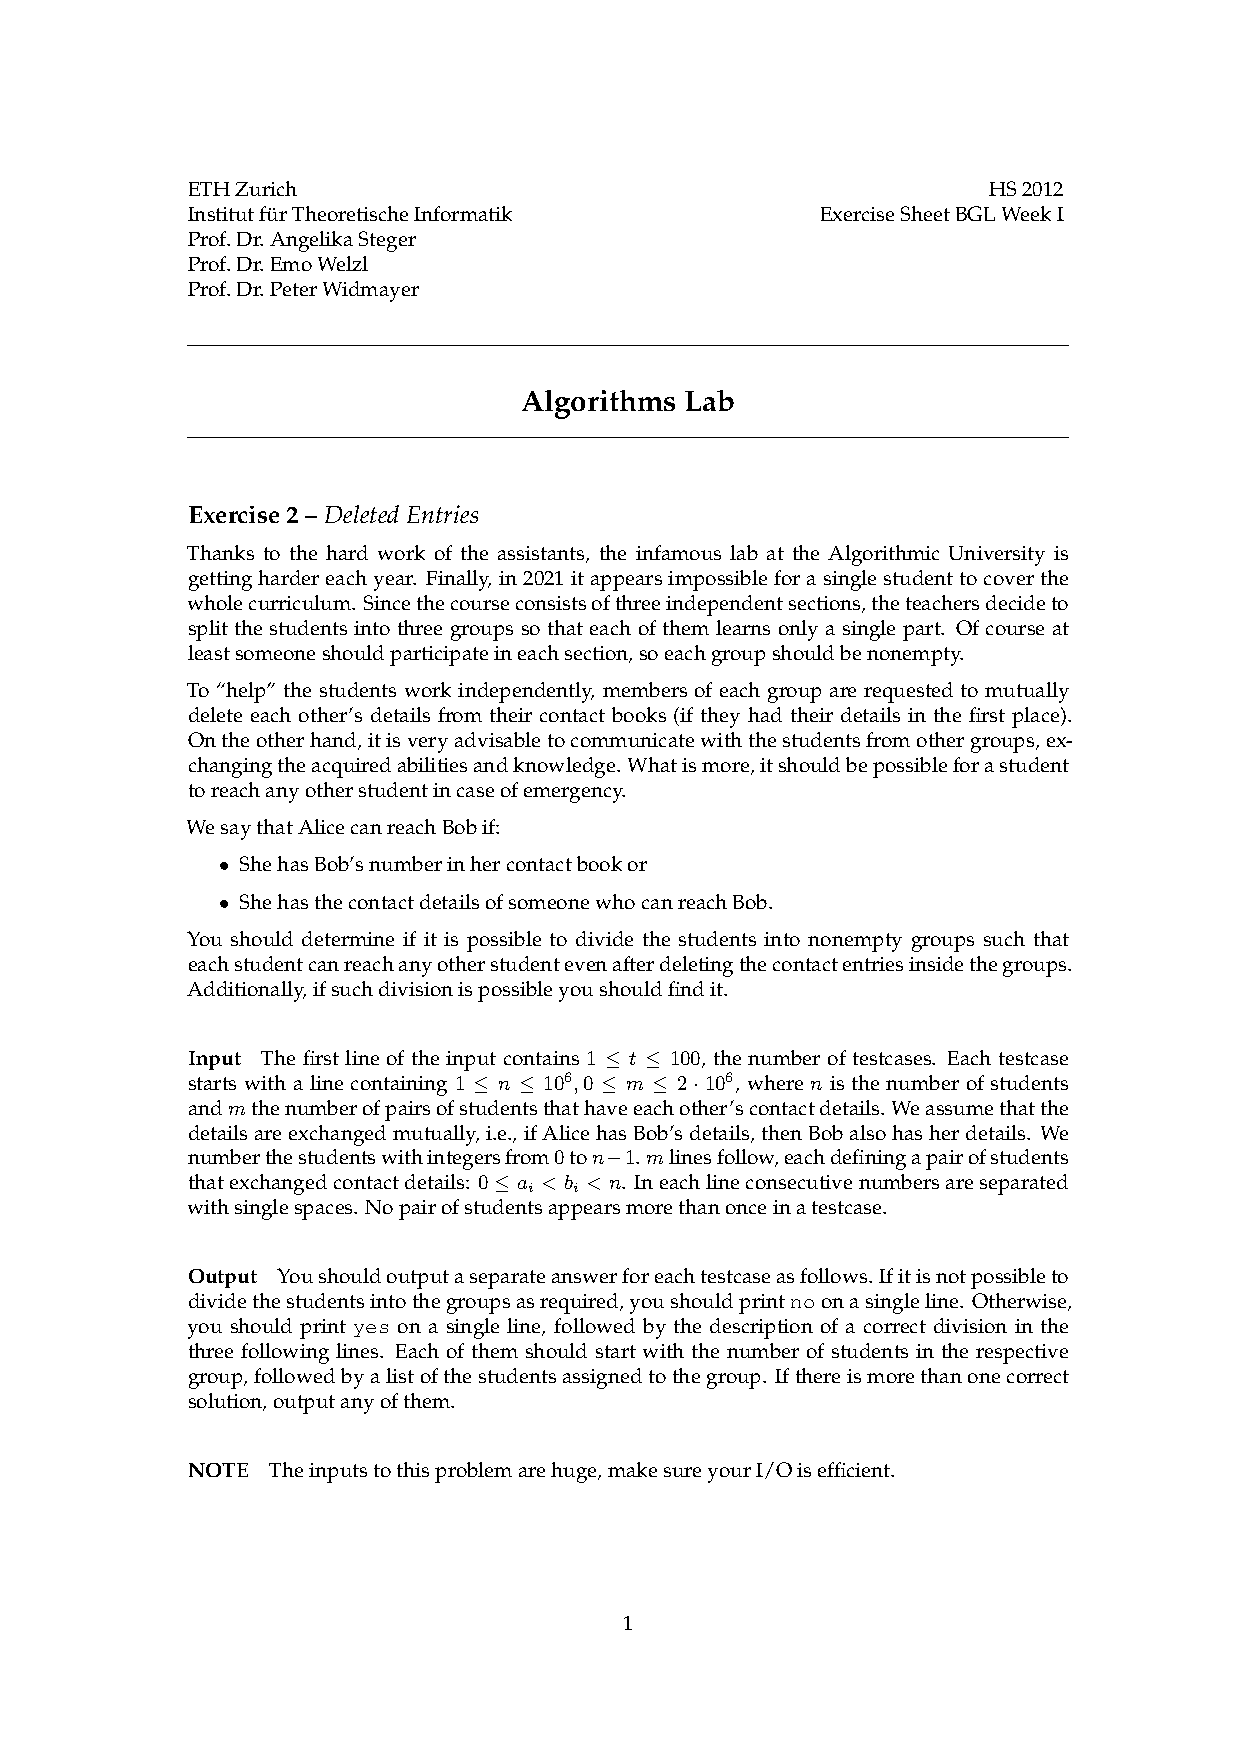
\includepdf{./week_4_bgl_introduction/2_deleted_entries/deleted_entries.pdf}
\lstinputlisting{./week_4_bgl_introduction/2_deleted_entries/main.cpp}
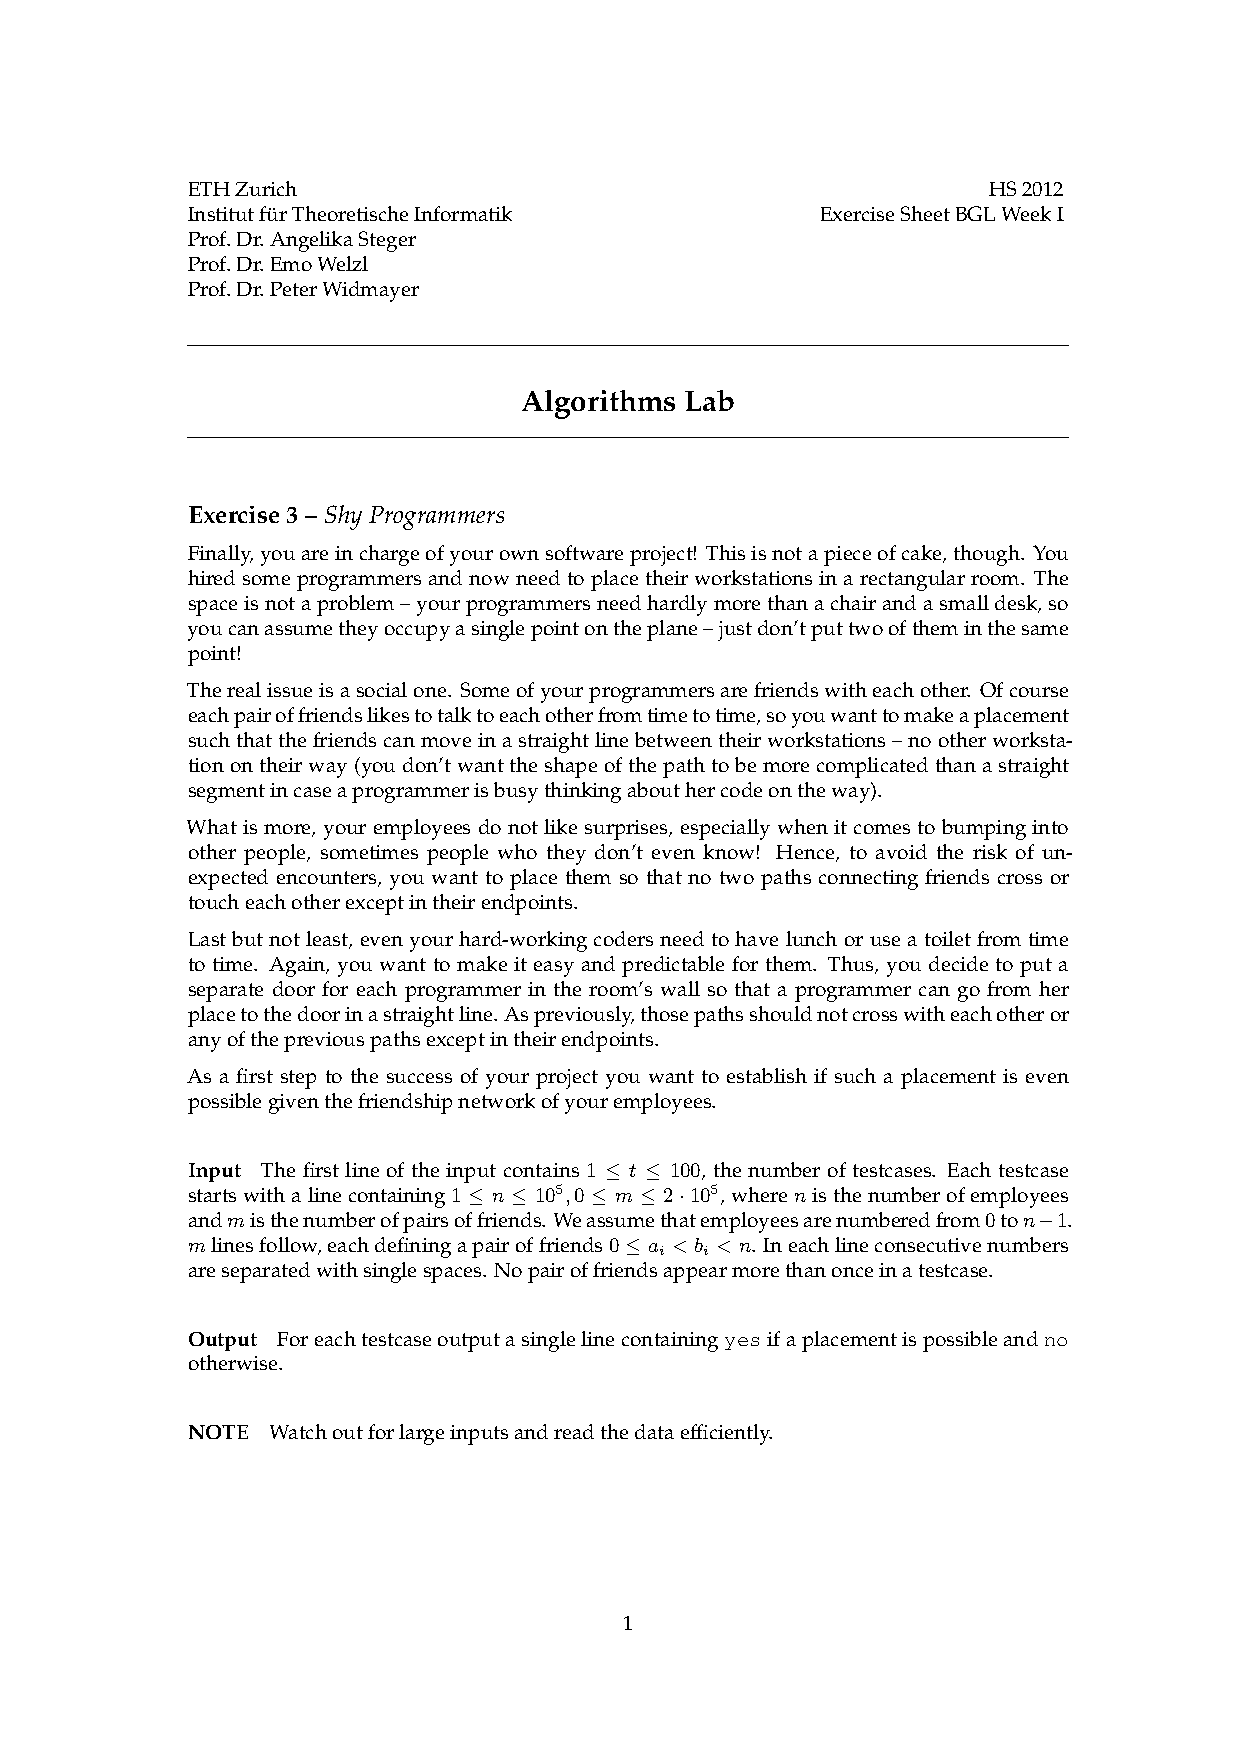
\includepdf{./week_4_bgl_introduction/3_shy_programmers/this.pdf}
\lstinputlisting{./week_4_bgl_introduction/3_shy_programmers/shy_programmers/main.cpp}

\newpage
\part{Week 5 - Flows}
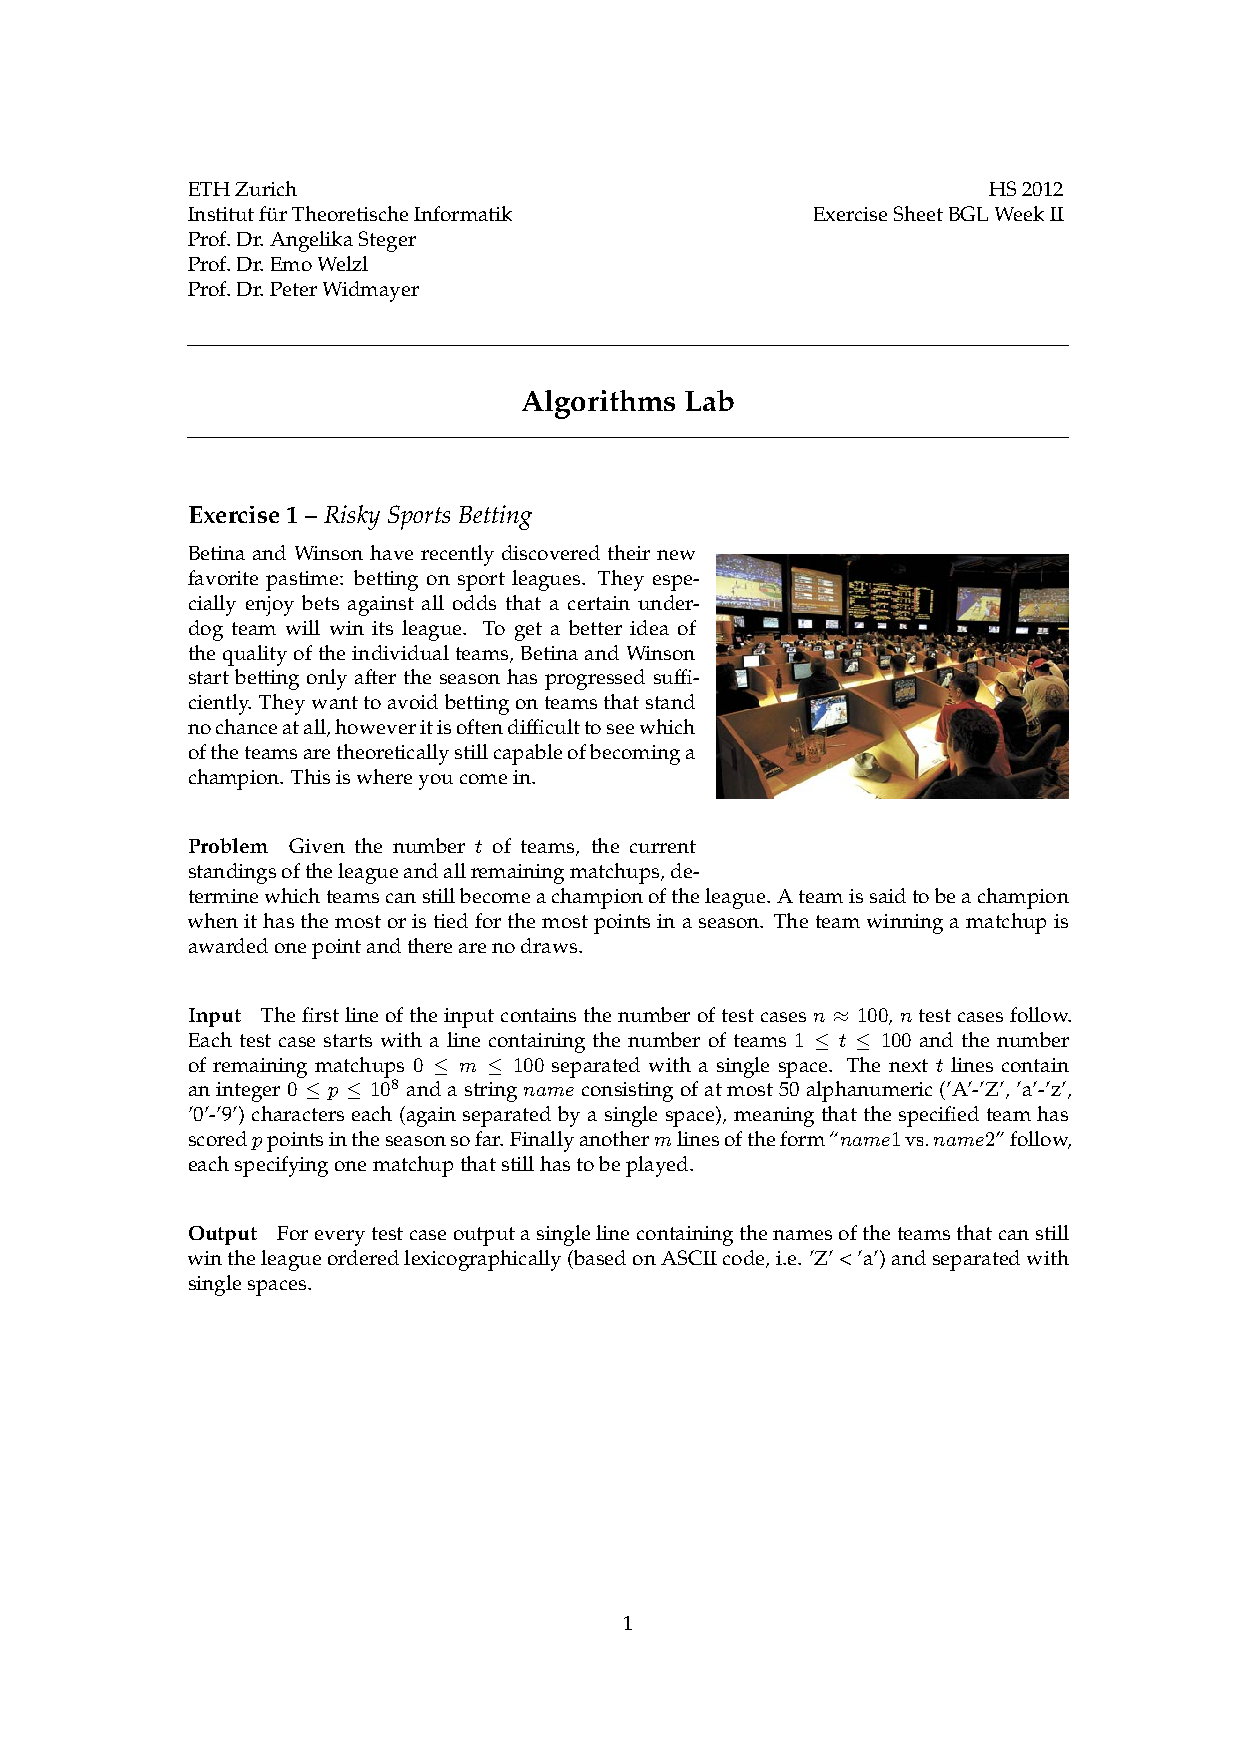
\includepdf{./week_5_flows/0_tournament/tournament.pdf}
\lstinputlisting{./week_5_flows/0_tournament/tournament/main.cpp}
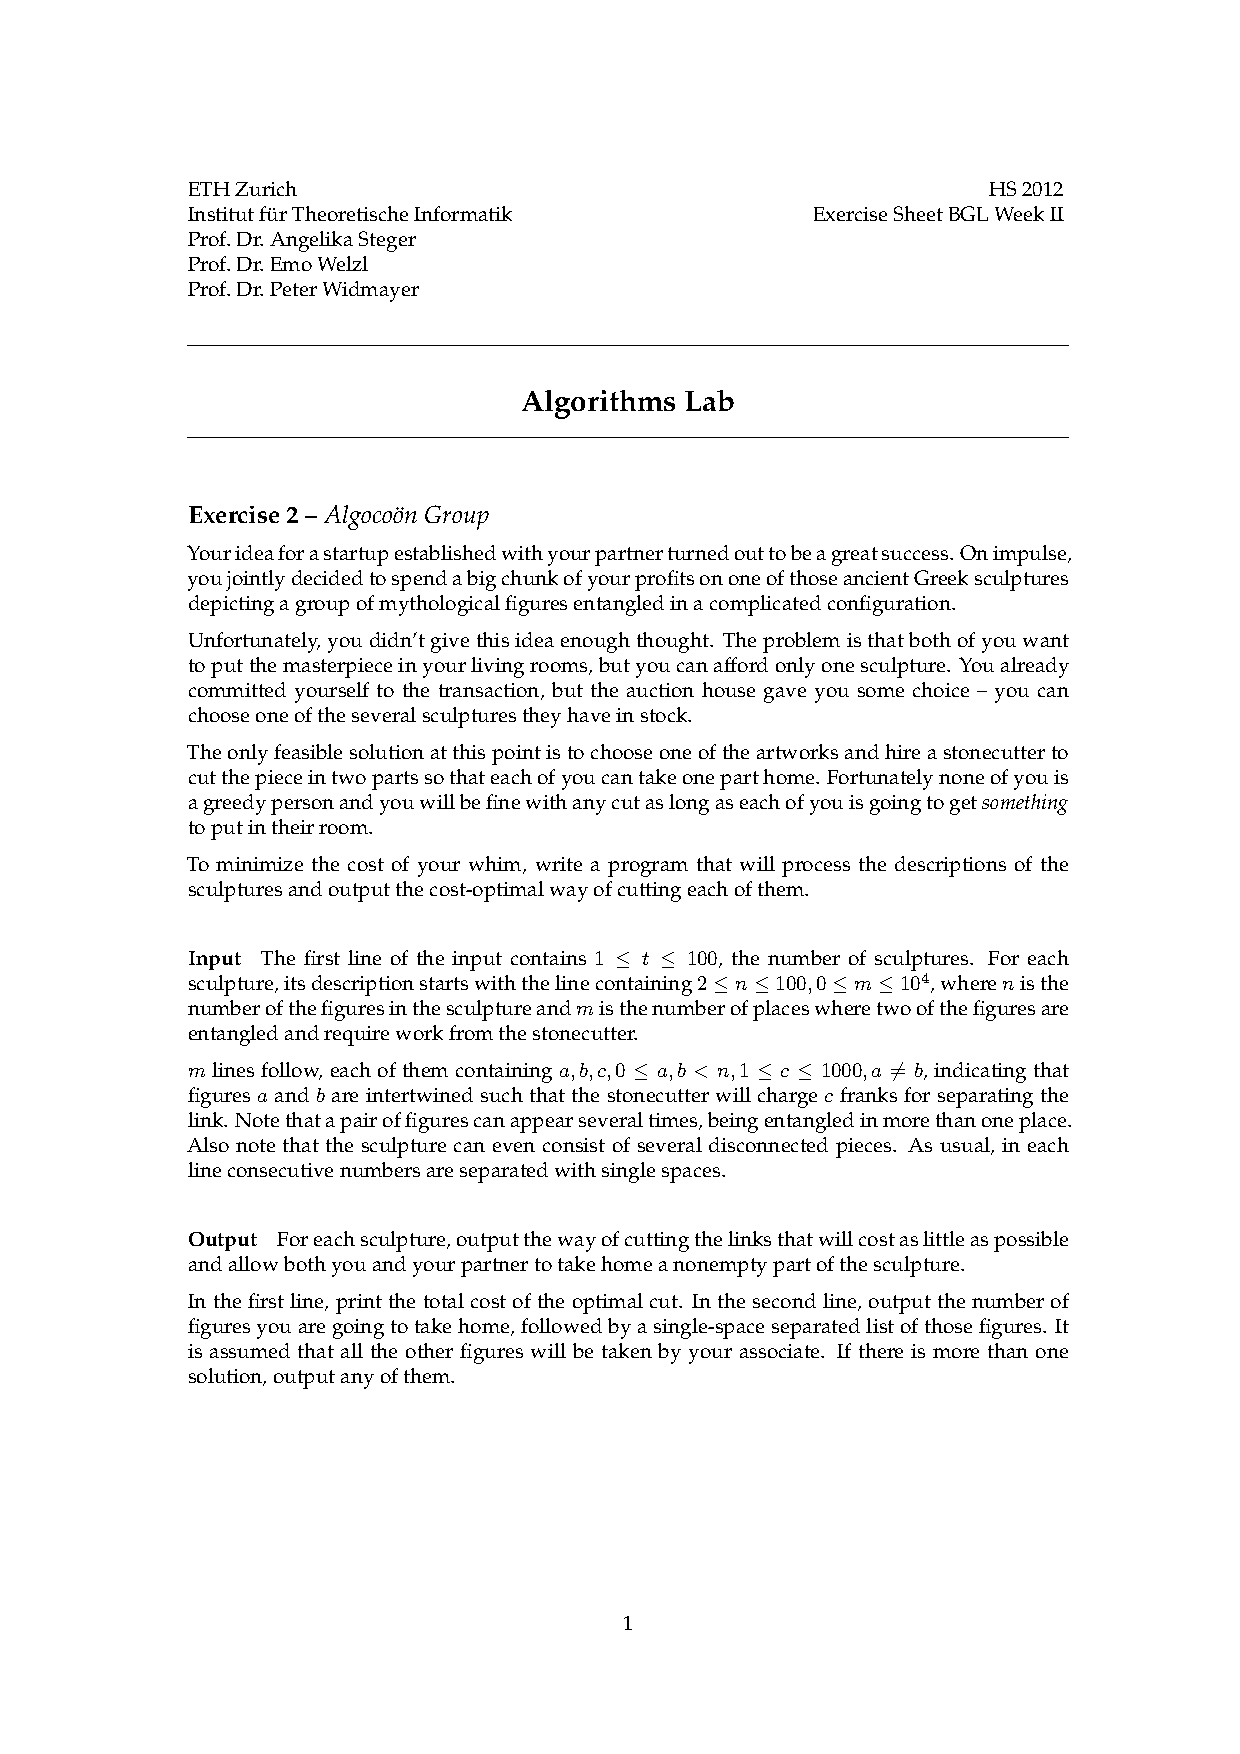
\includepdf{./week_5_flows/1_algocon_group/this.pdf}
\lstinputlisting{./week_5_flows/1_algocon_group/algocon/main.cpp}
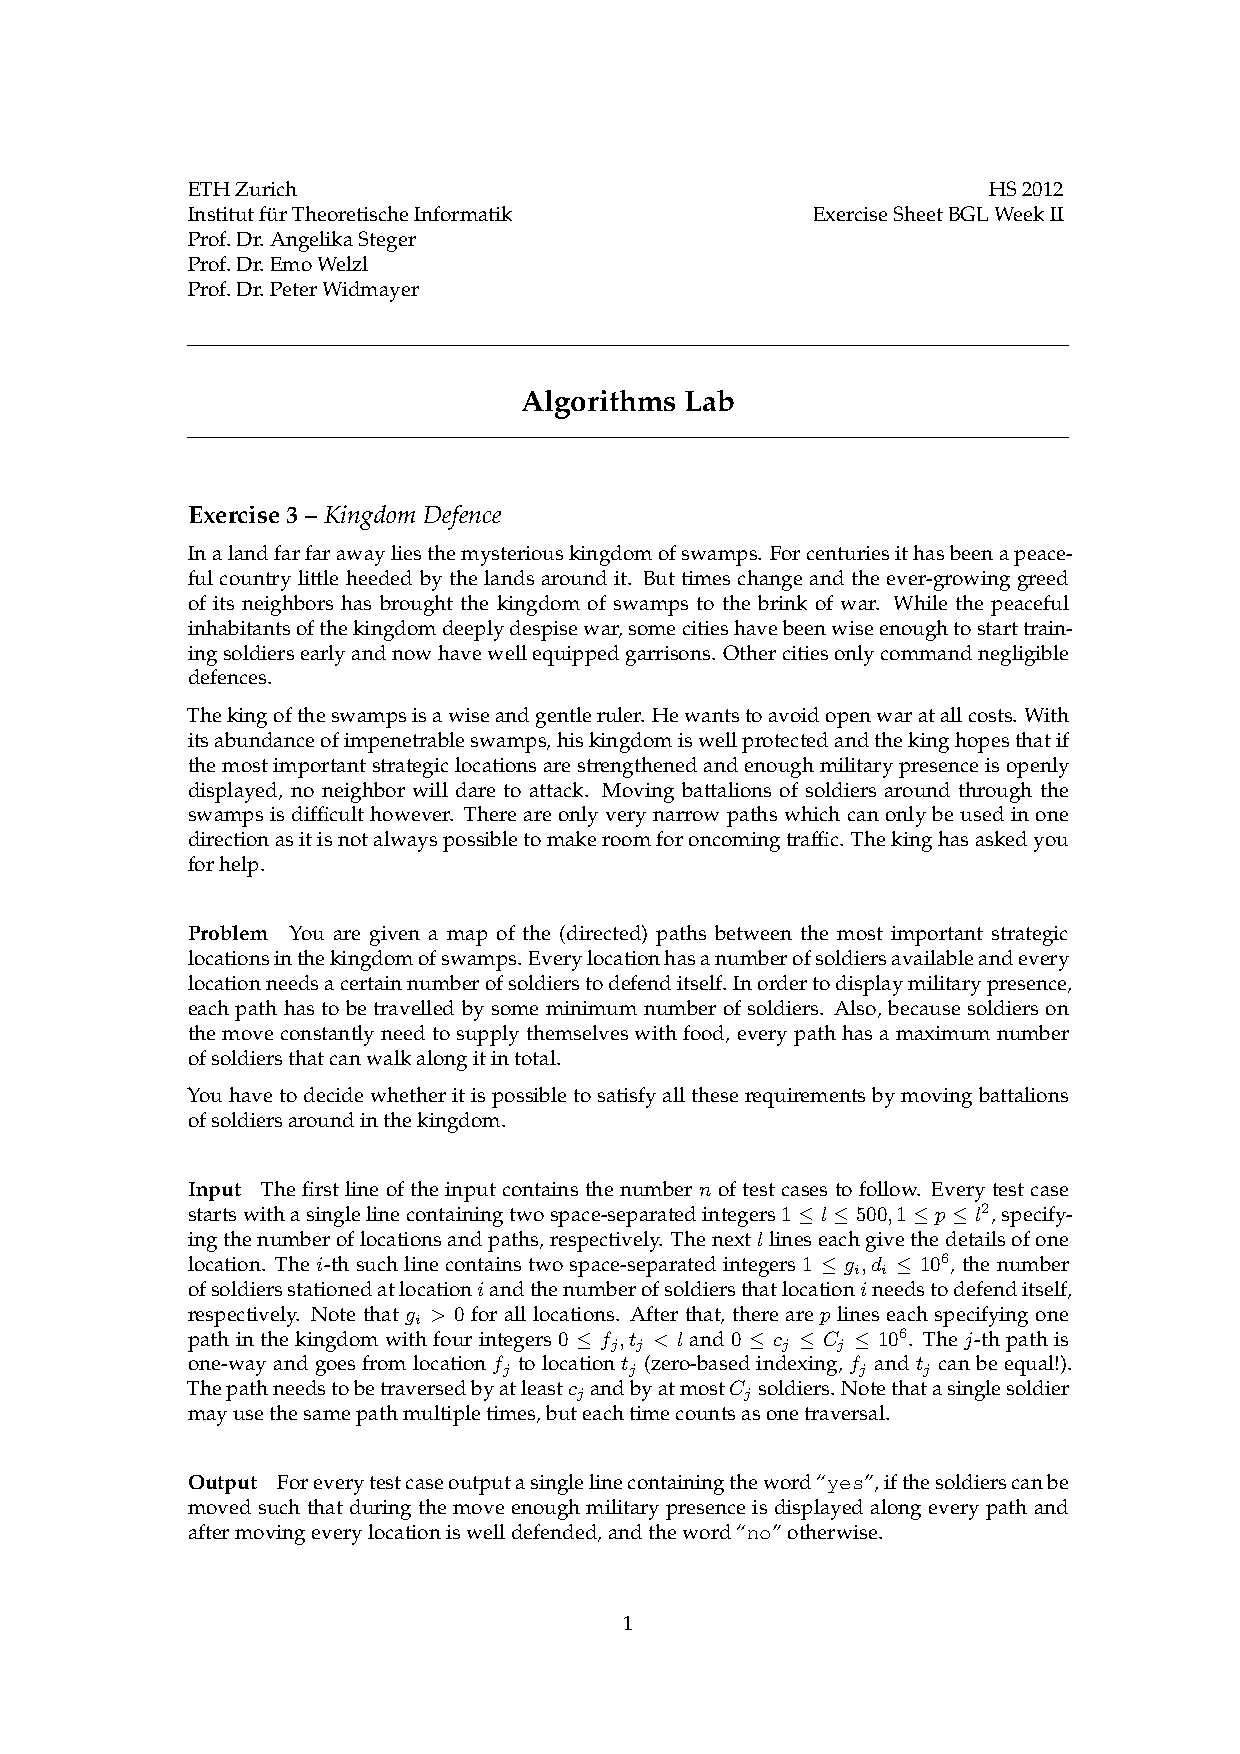
\includepdf{./week_5_flows/2_defence/defence.pdf}
\lstinputlisting{./week_5_flows/2_defence/defence/main.cpp}

\newpage
\part{Week 6 - Matchings}
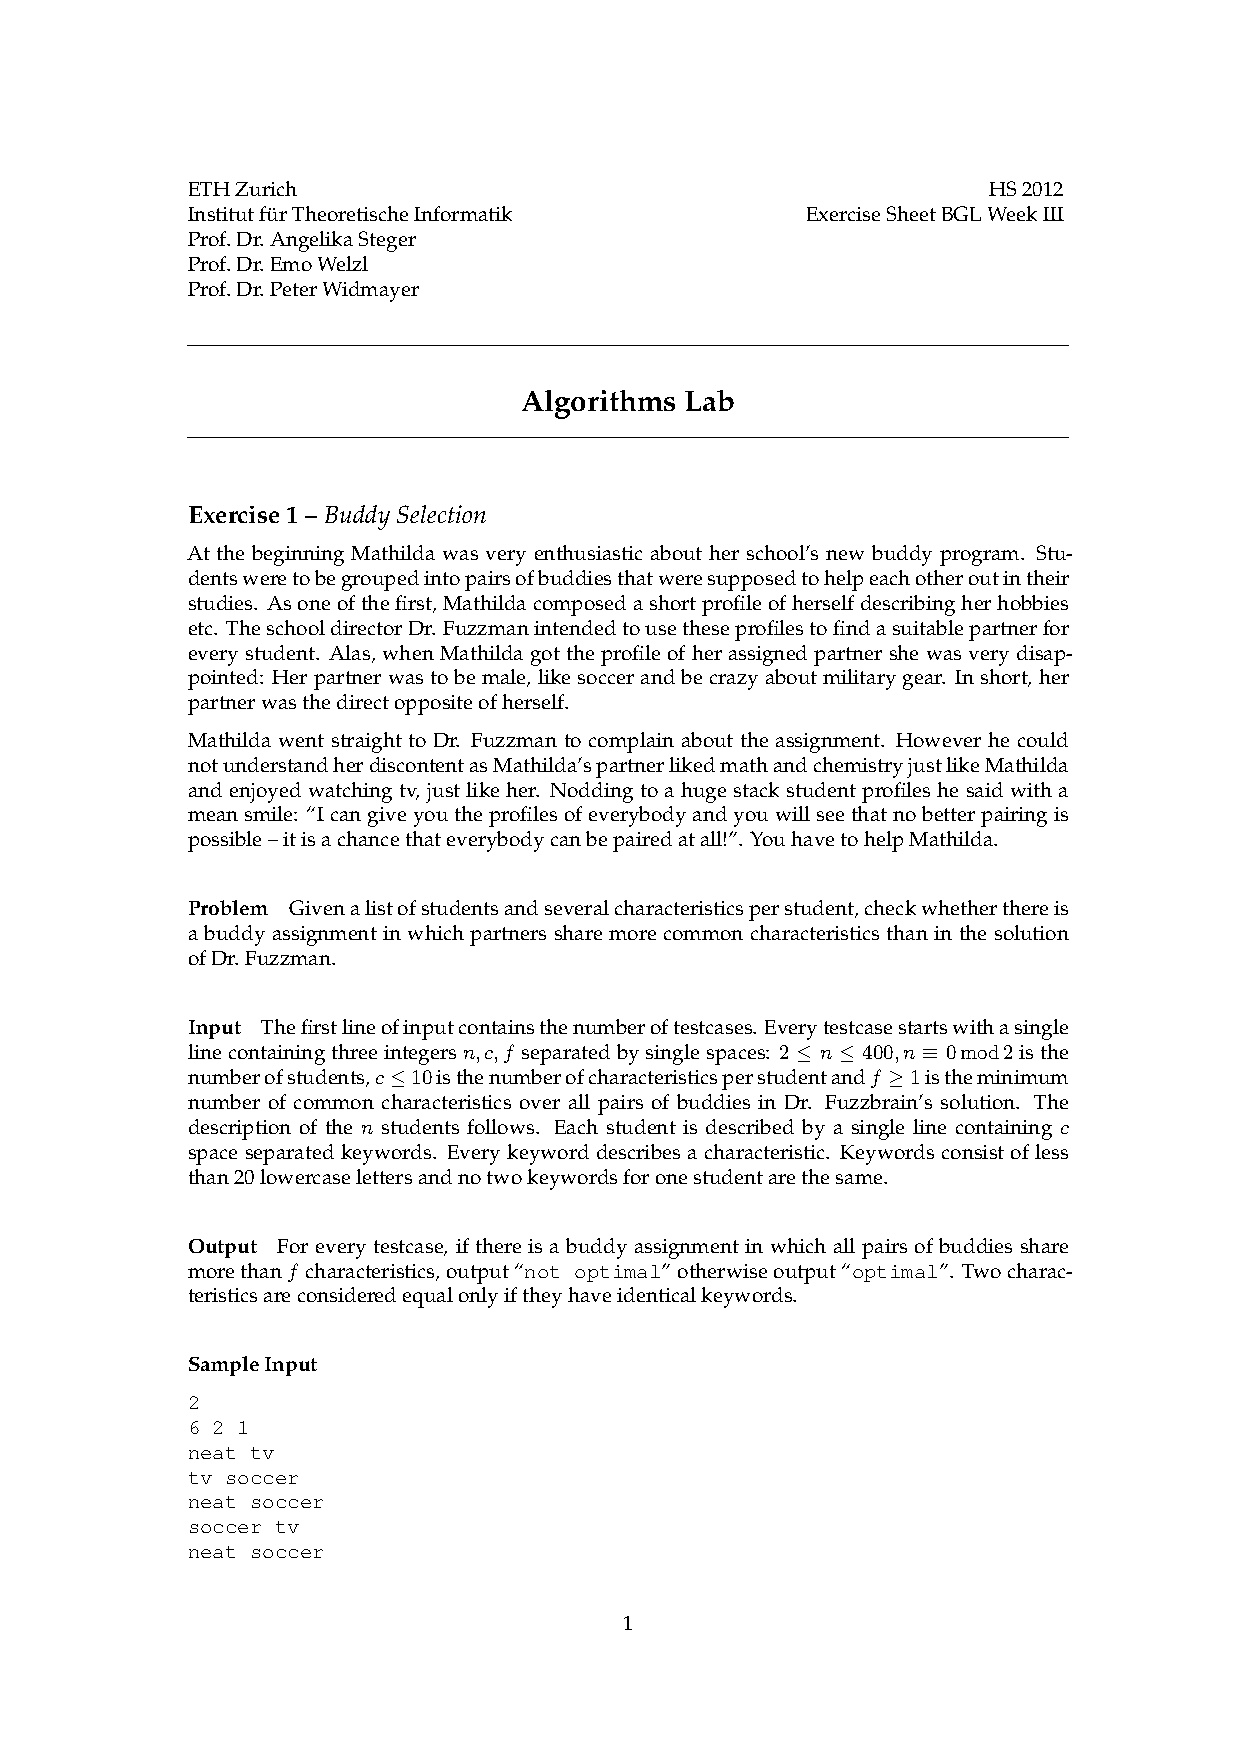
\includepdf{./week_6_matchings/0_buddies/buddies.pdf}
\lstinputlisting{./week_6_matchings/0_buddies/buddies/main.cpp}
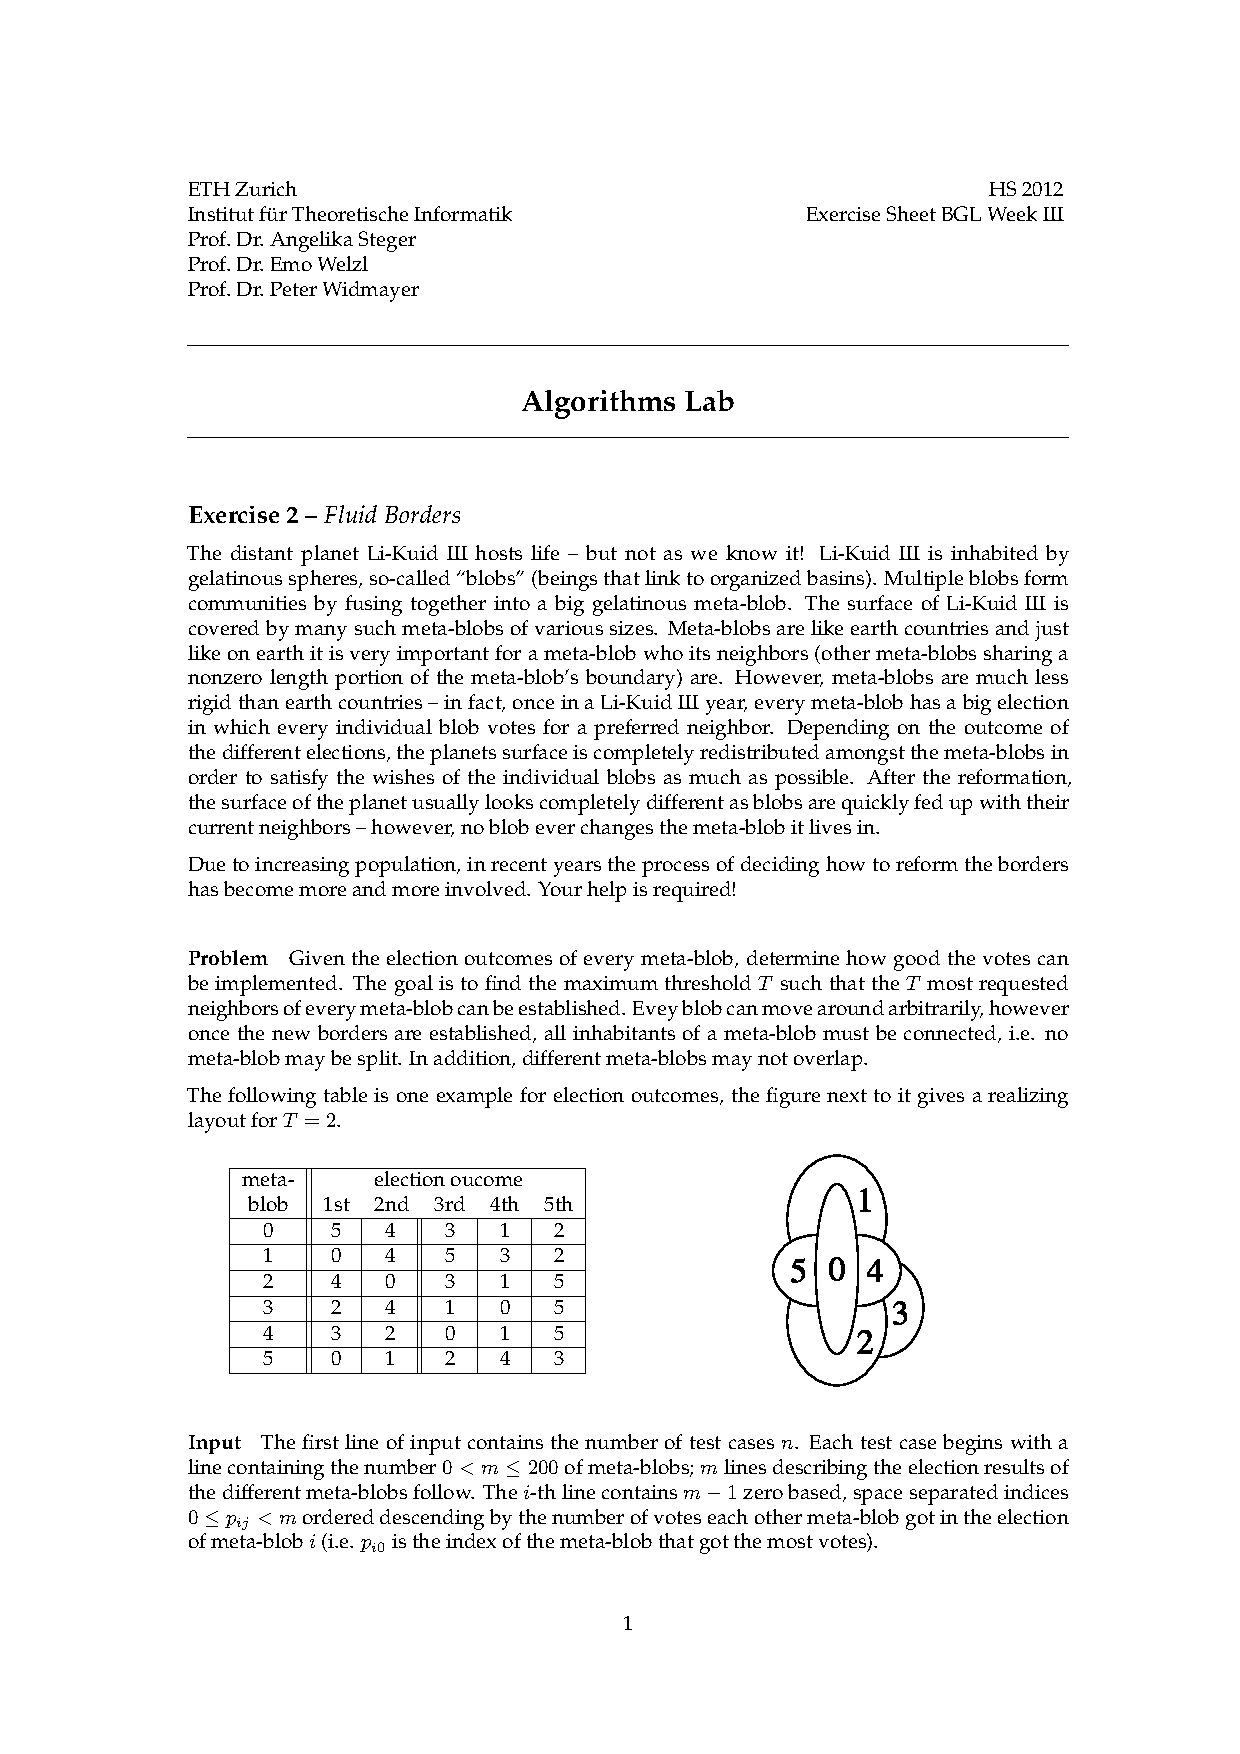
\includepdf{./week_6_matchings/1_borders/borders.pdf}
\lstinputlisting{./week_6_matchings/1_borders/borders/main.cpp}
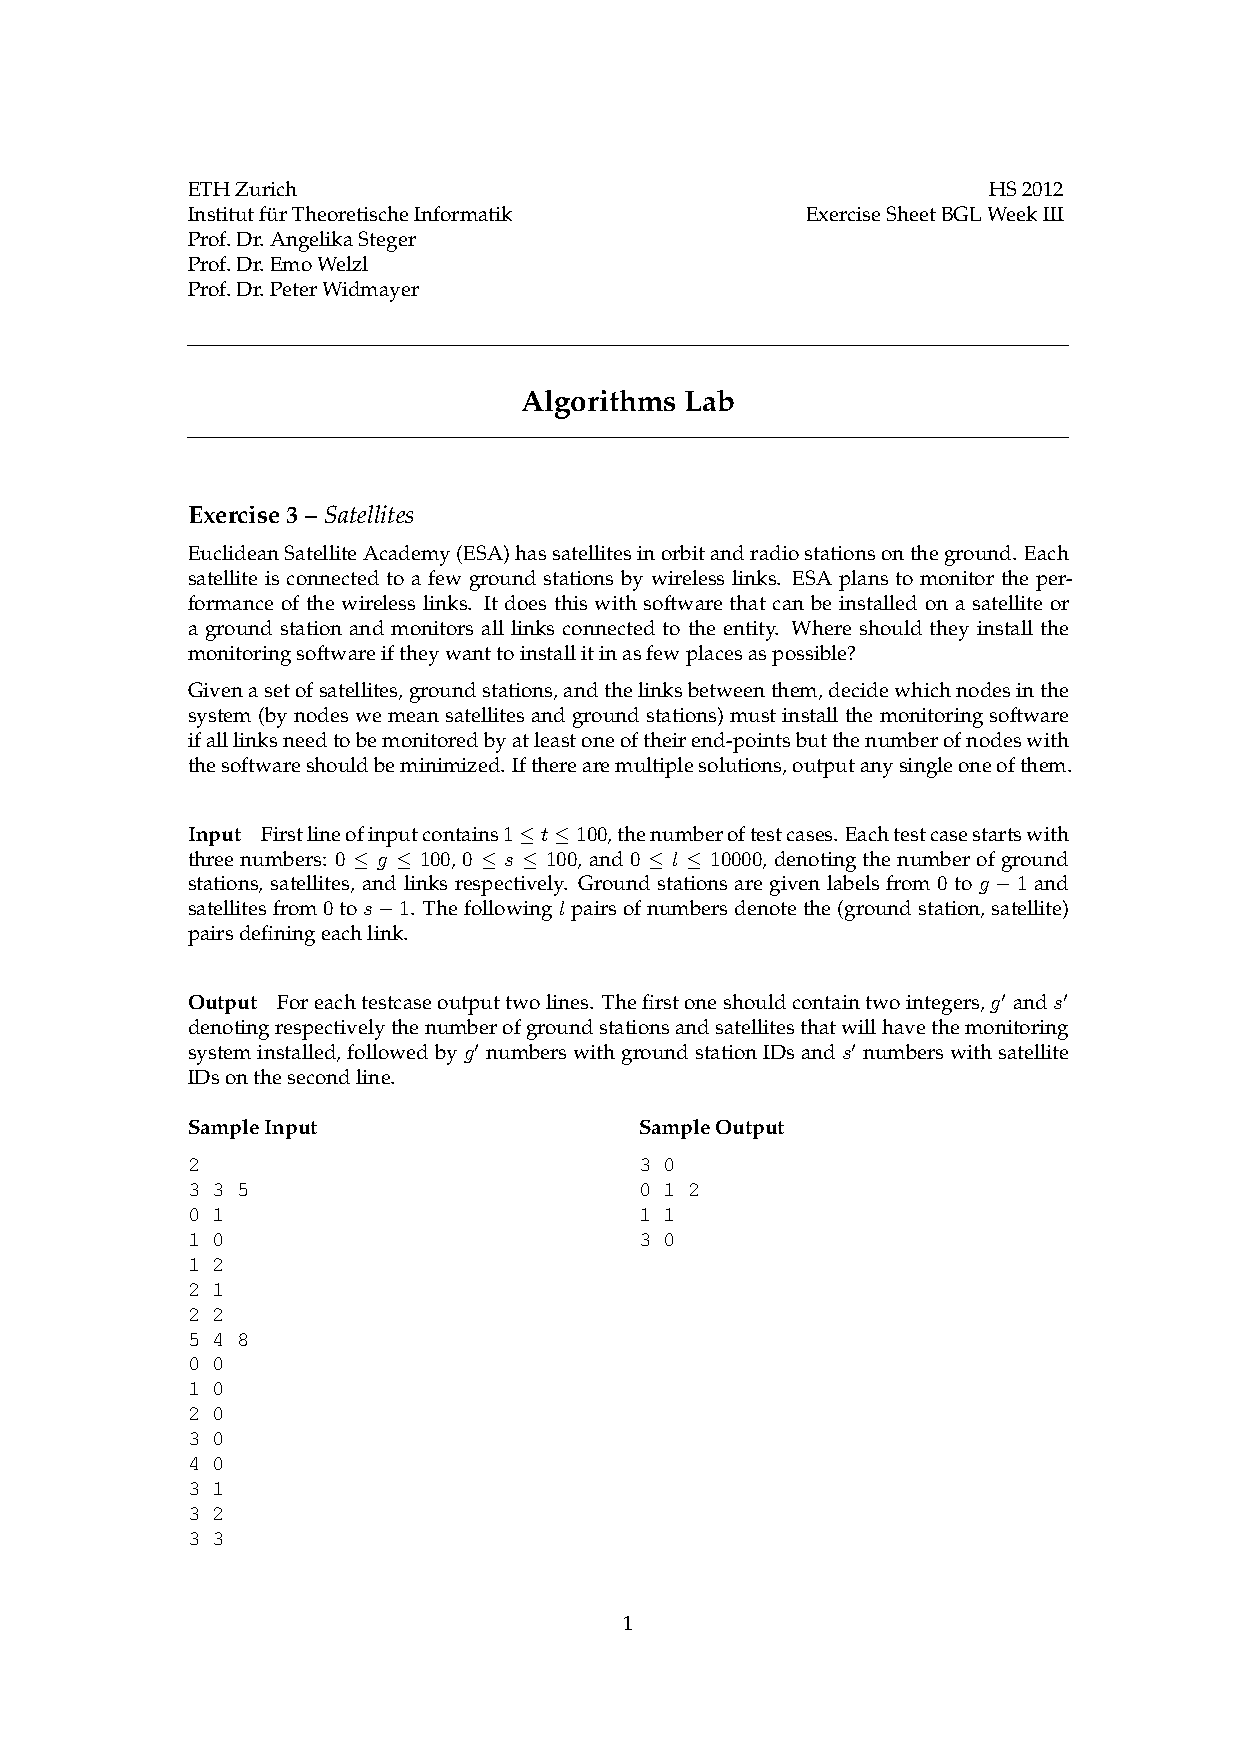
\includepdf{./week_6_matchings/2_satellites/satellites.pdf}
\lstinputlisting{./week_6_matchings/2_satellites/satellites/main.cpp}
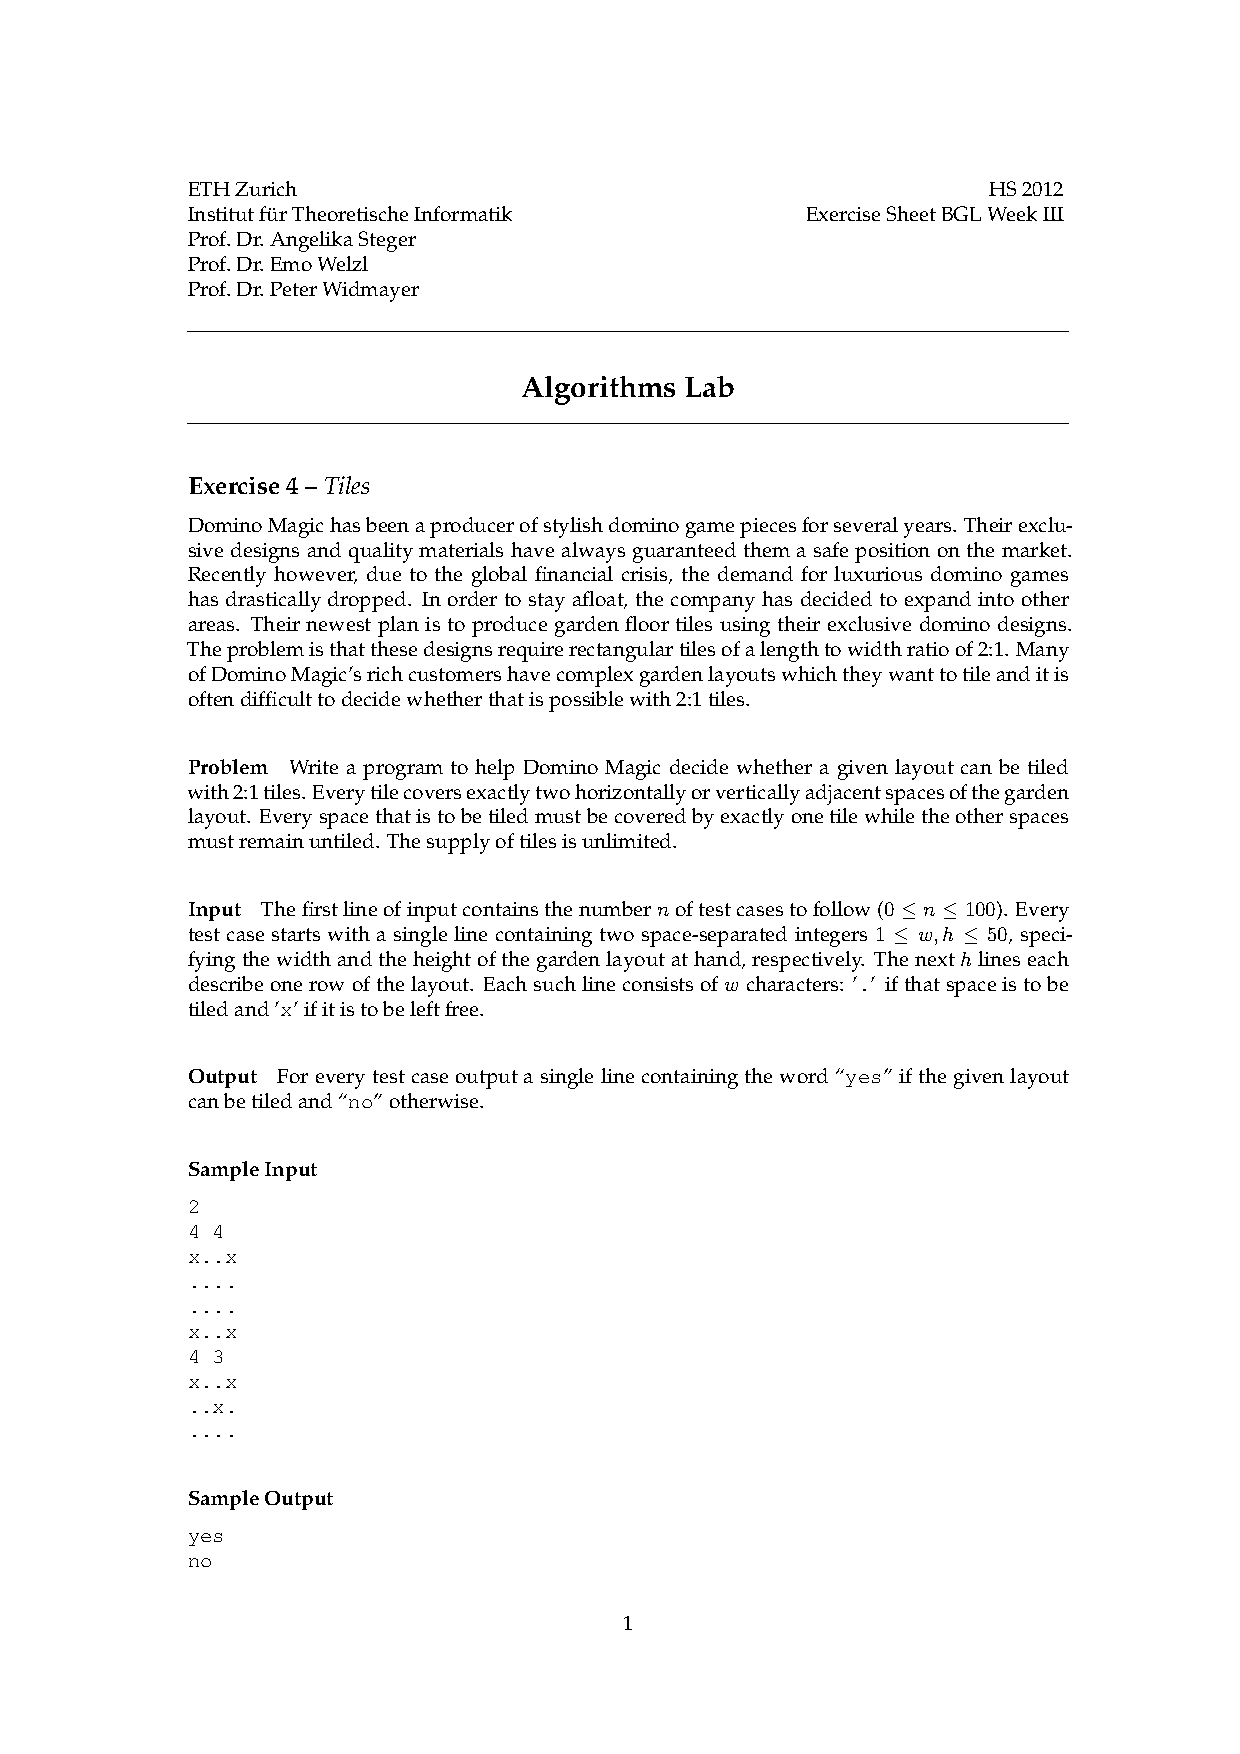
\includepdf{./week_6_matchings/3_tiles/tiles.pdf}
\lstinputlisting{./week_6_matchings/3_tiles/tiles/main.cpp}

\newpage
\part{Week 7 - Mixed}
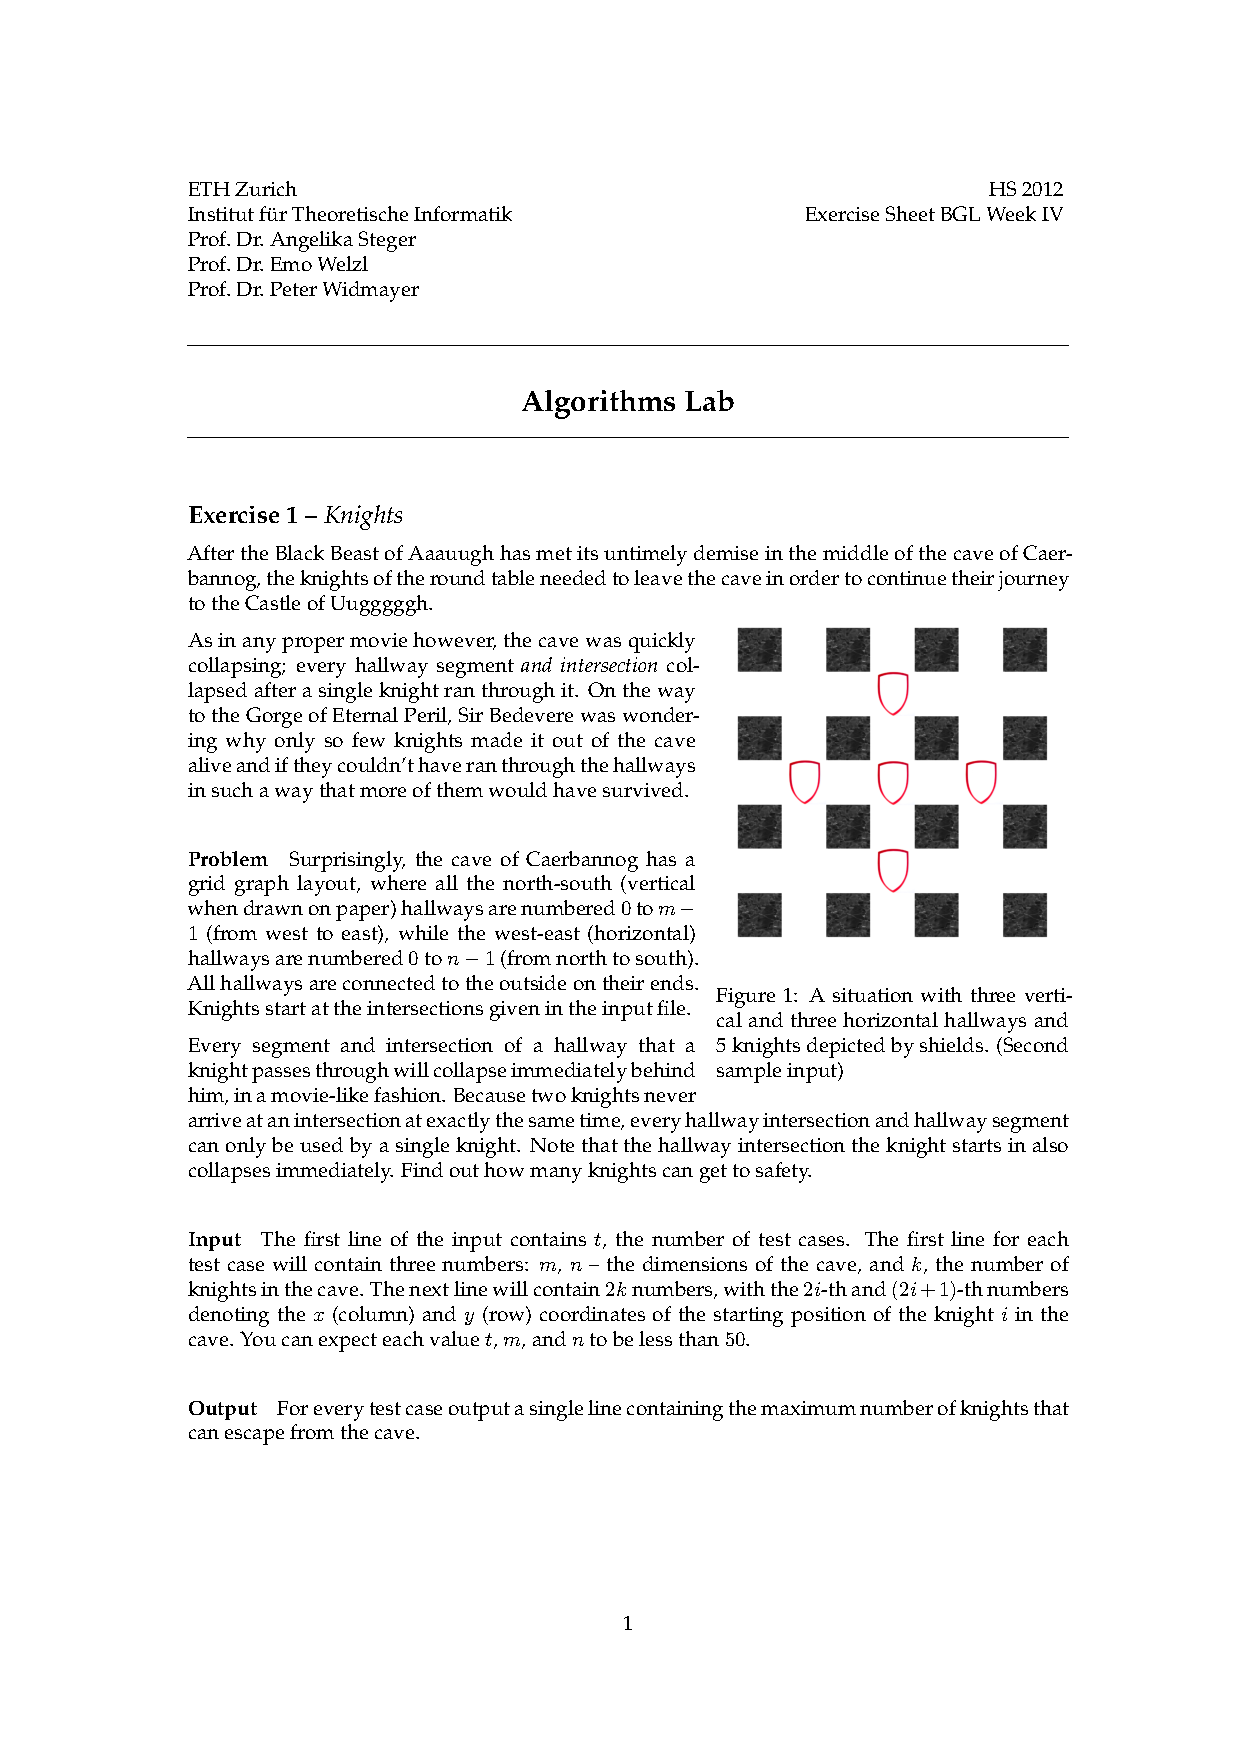
\includepdf{./week_7_mixed/0_knights/knights.pdf}
\lstinputlisting{./week_7_mixed/0_knights/knights/main.cpp}
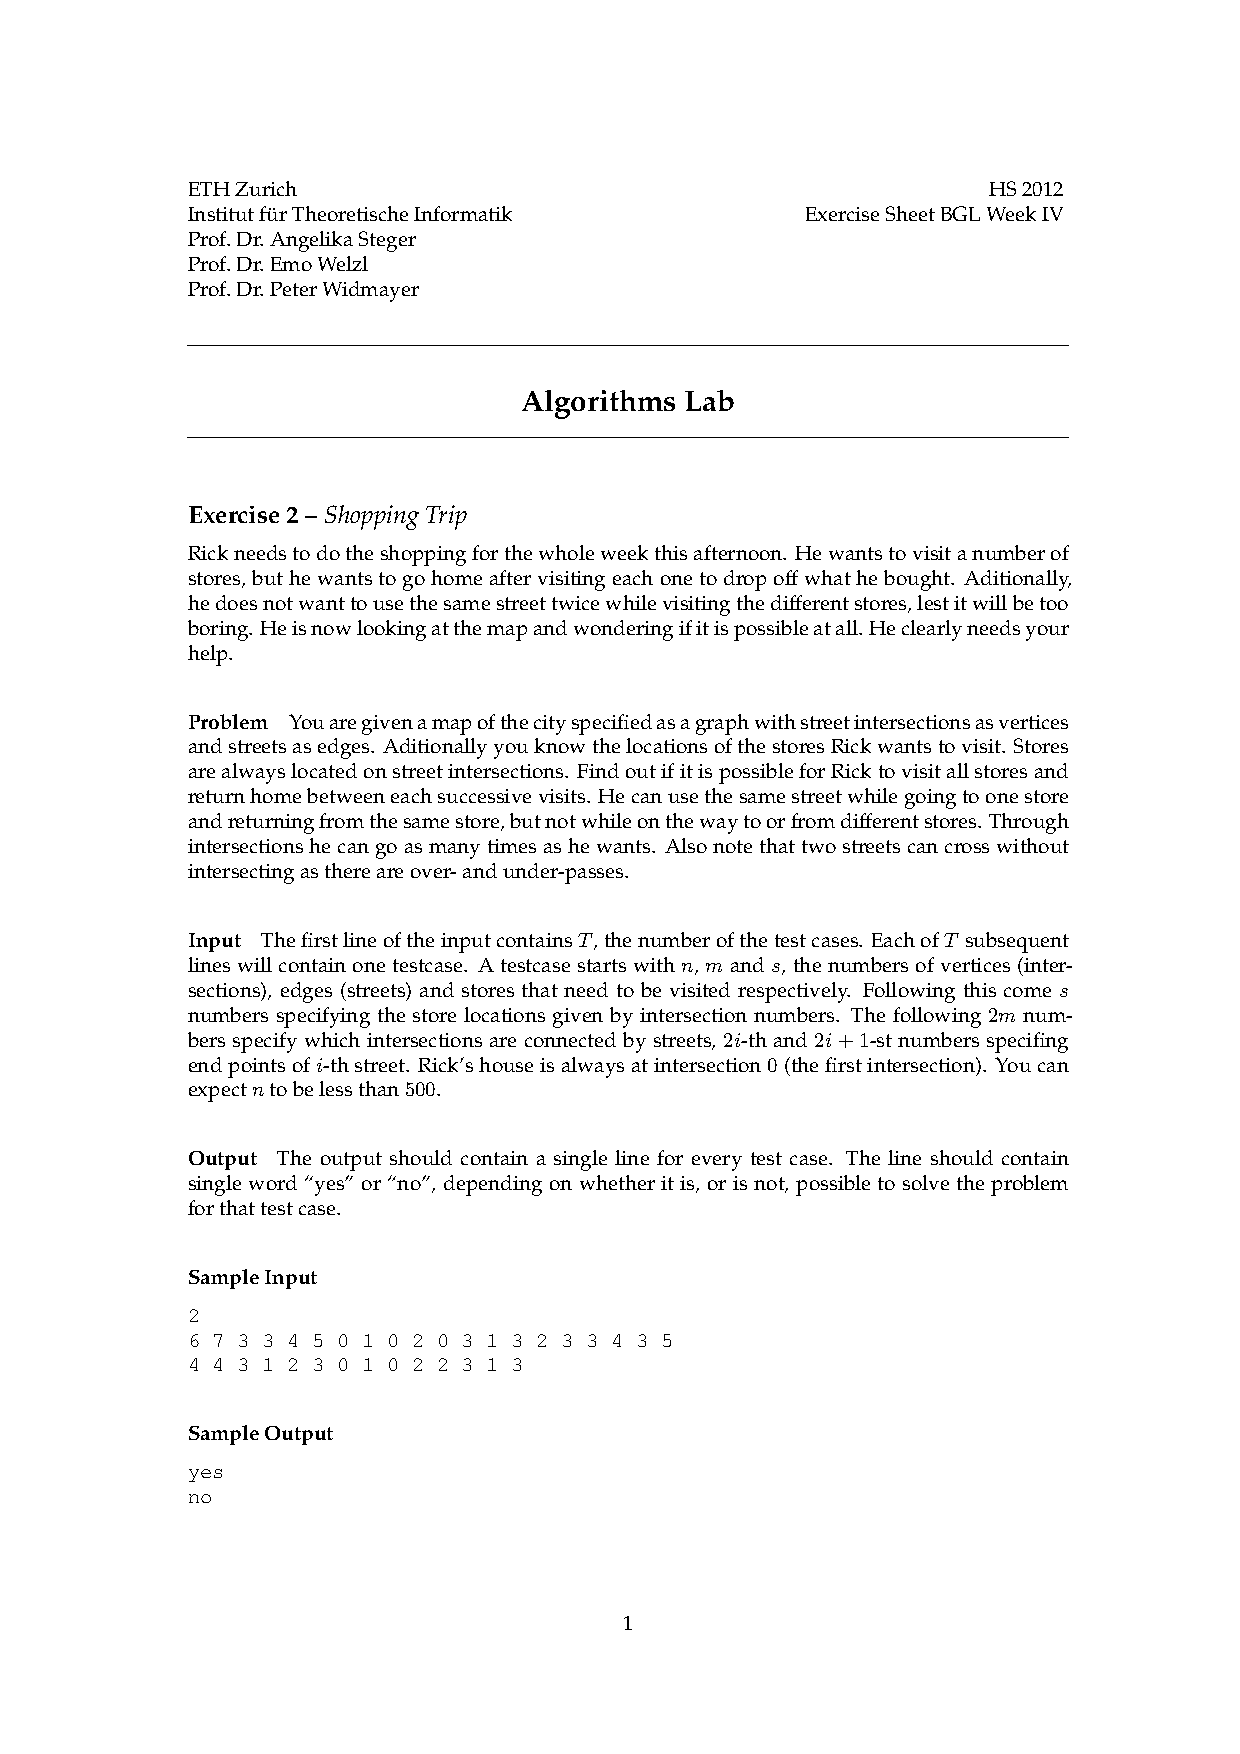
\includepdf{./week_7_mixed/1_shopping/shopping.pdf}
%\lstinputlisting{}
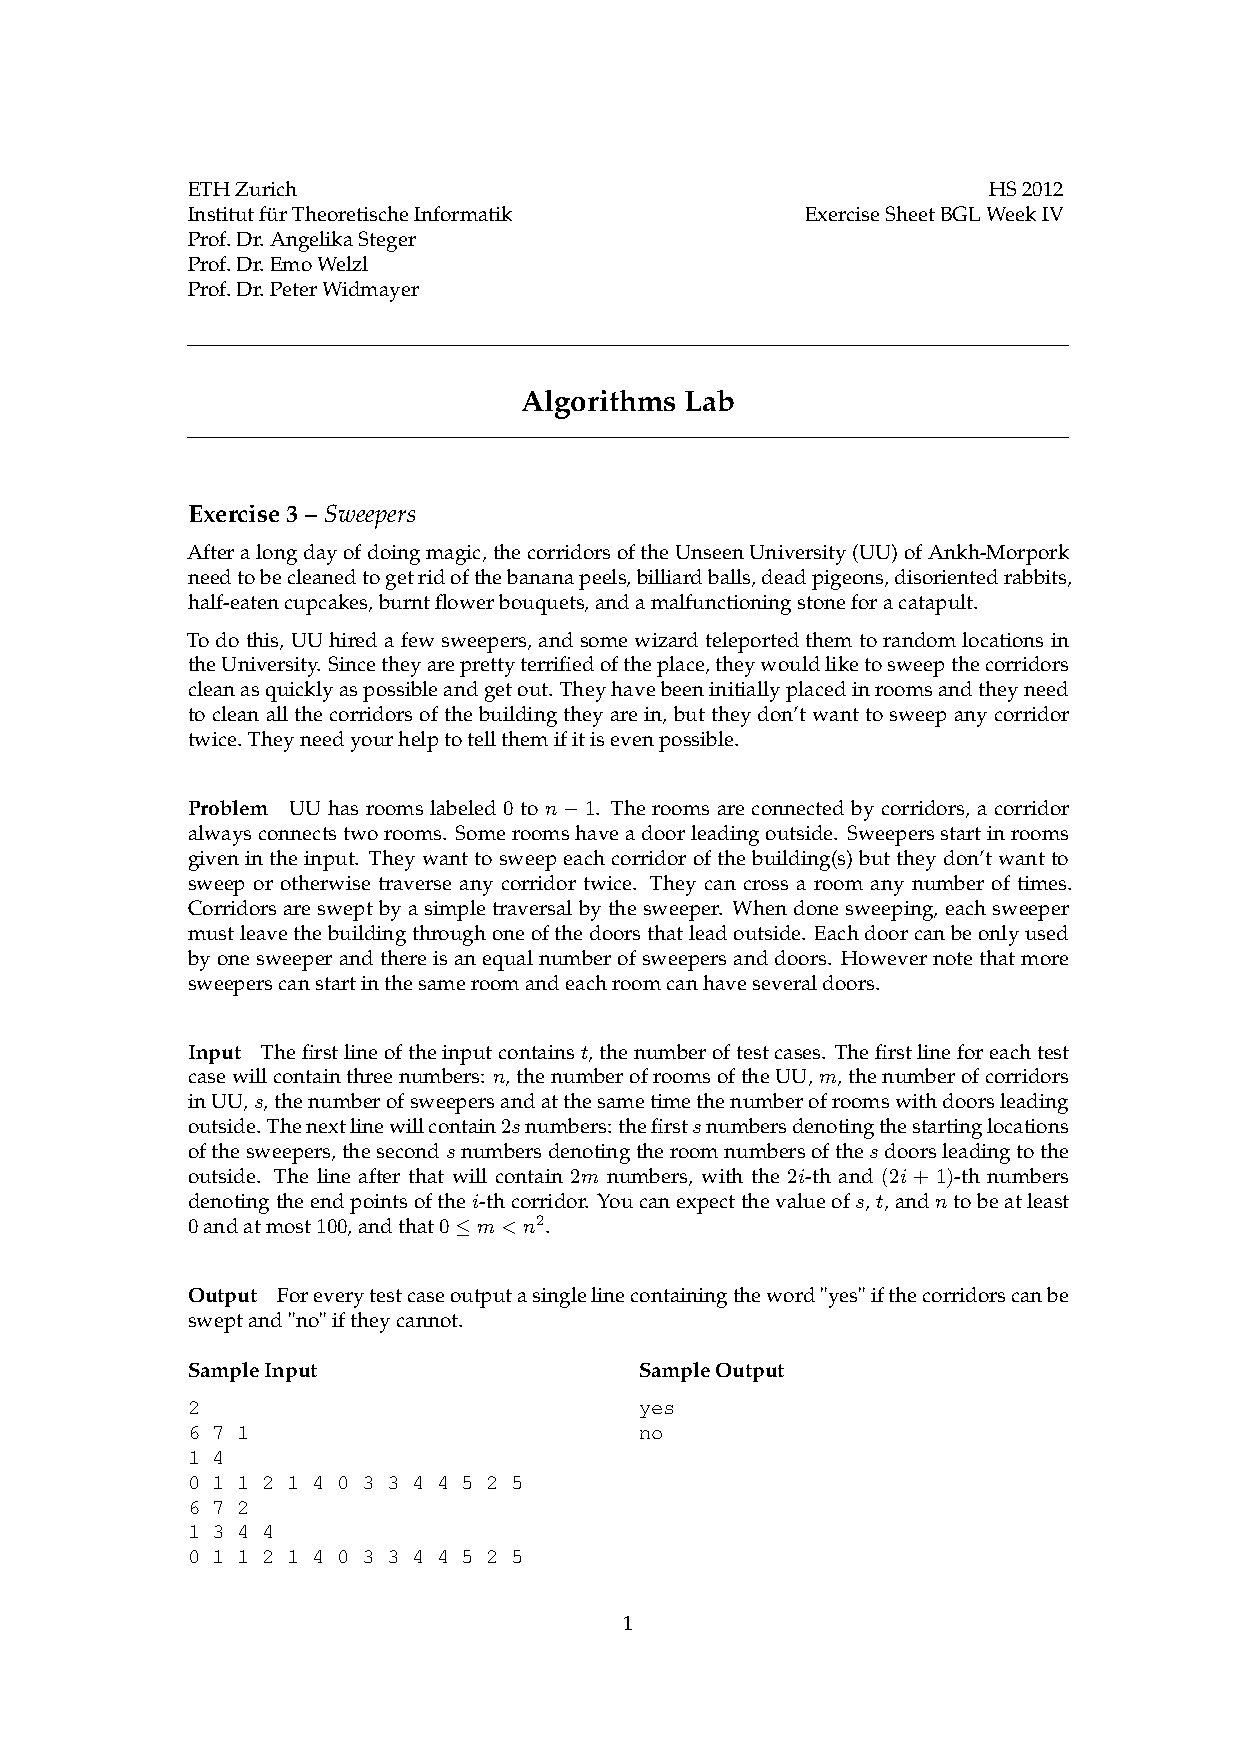
\includepdf{./week_7_mixed/2_sweepers/sweepers.pdf}
%\lstinputlisting{}
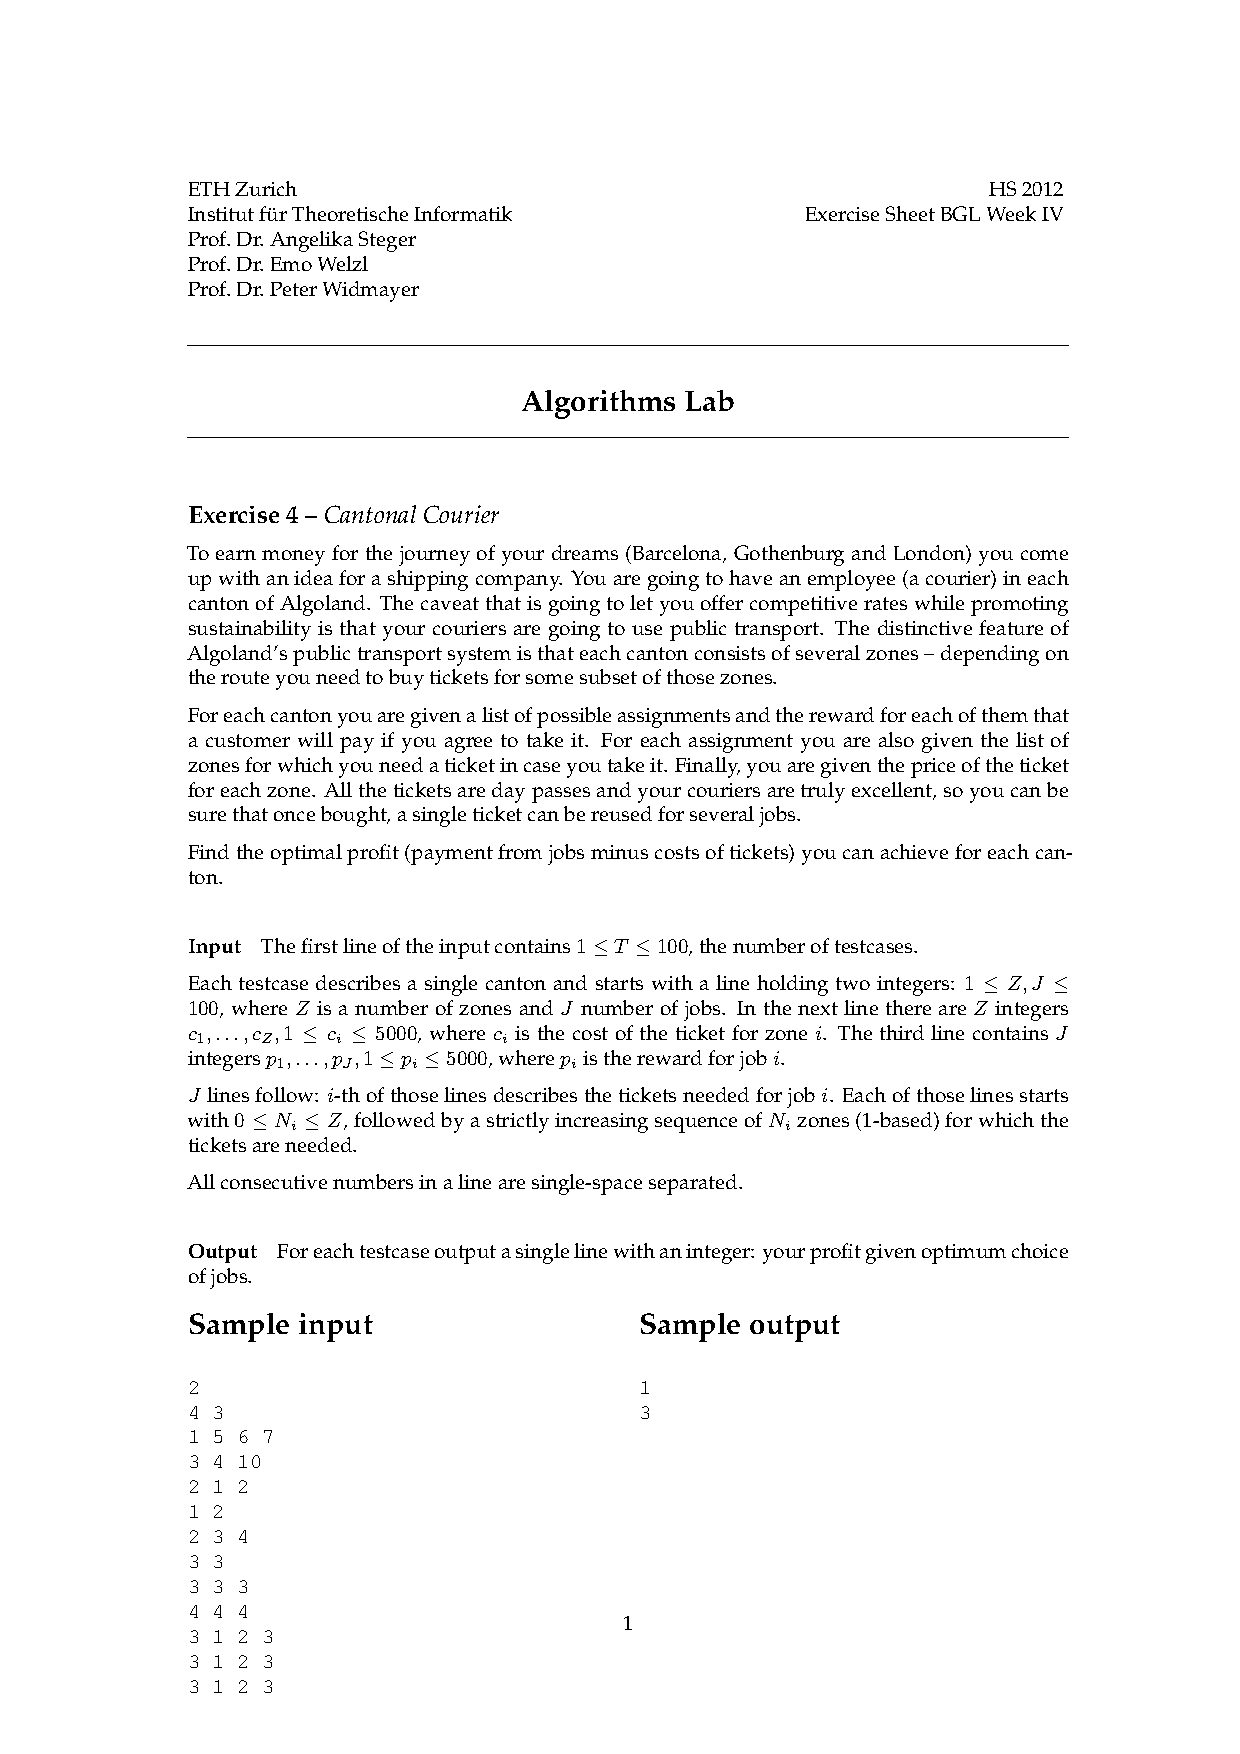
\includepdf{./week_7_mixed/3_courier/courier.pdf}
%\lstinputlisting{}

\newpage
\part{Week 8 - CGAL}
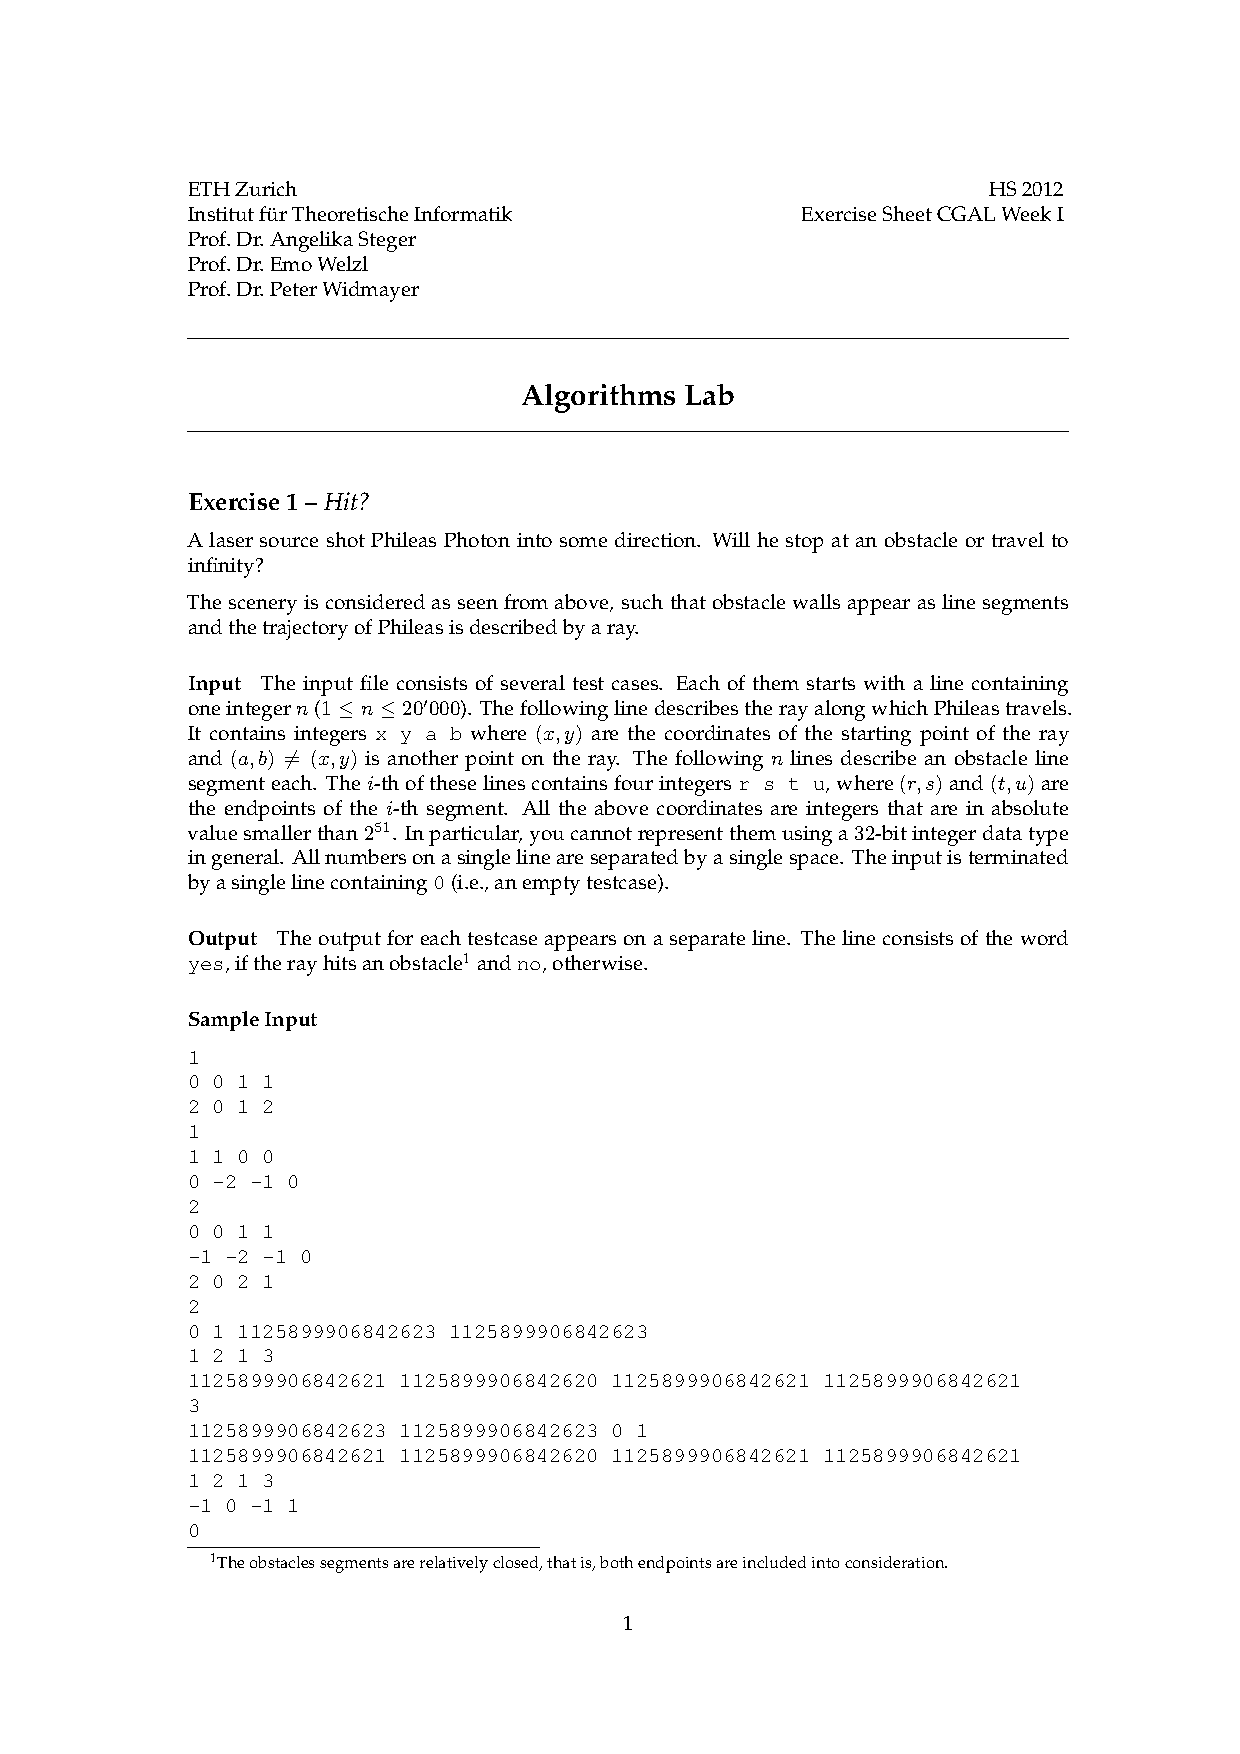
\includepdf{./week_8_cgal/0_hit/ex1.pdf}
\lstinputlisting{./week_8_cgal/0_hit/main.cpp}
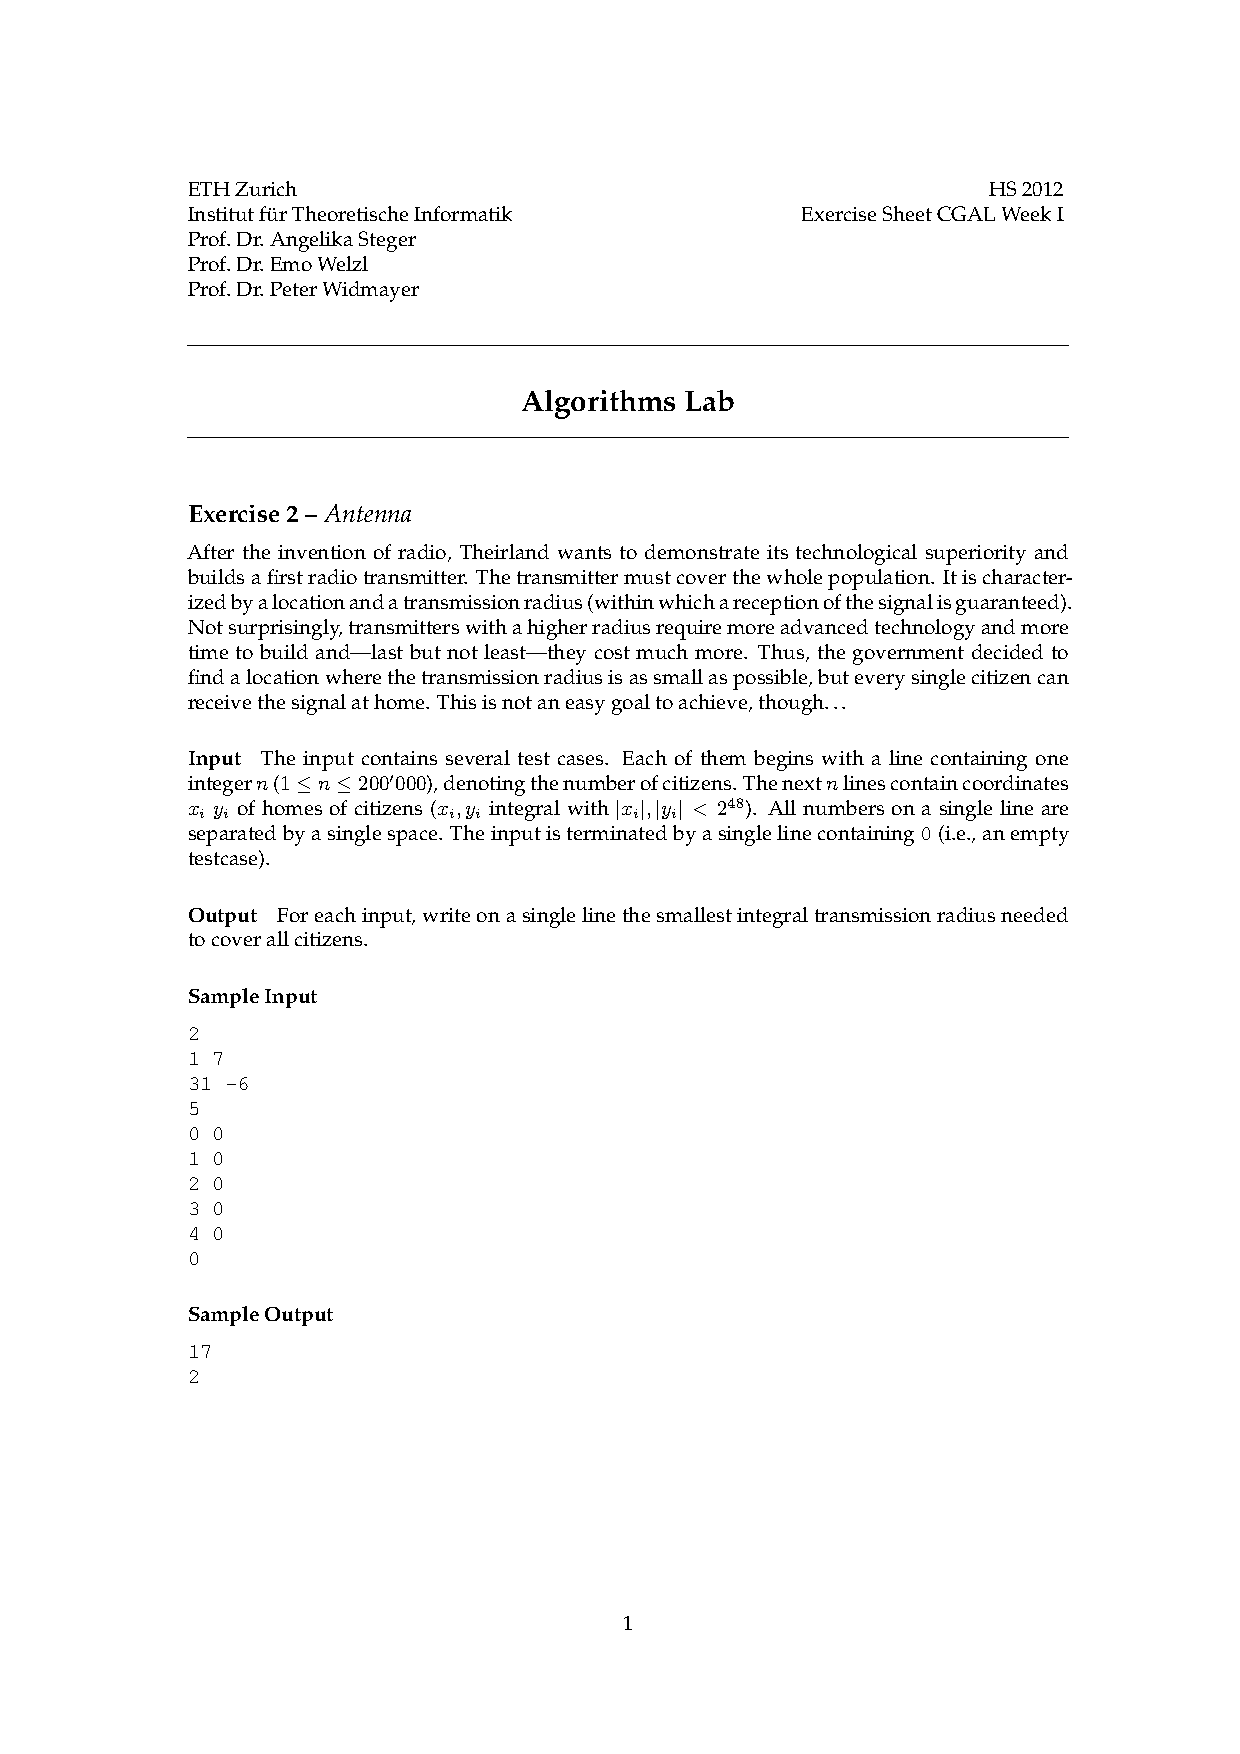
\includepdf{./week_8_cgal/1_antenna/ex2.pdf}
\lstinputlisting{./week_8_cgal/1_antenna/antenna/main.cpp}
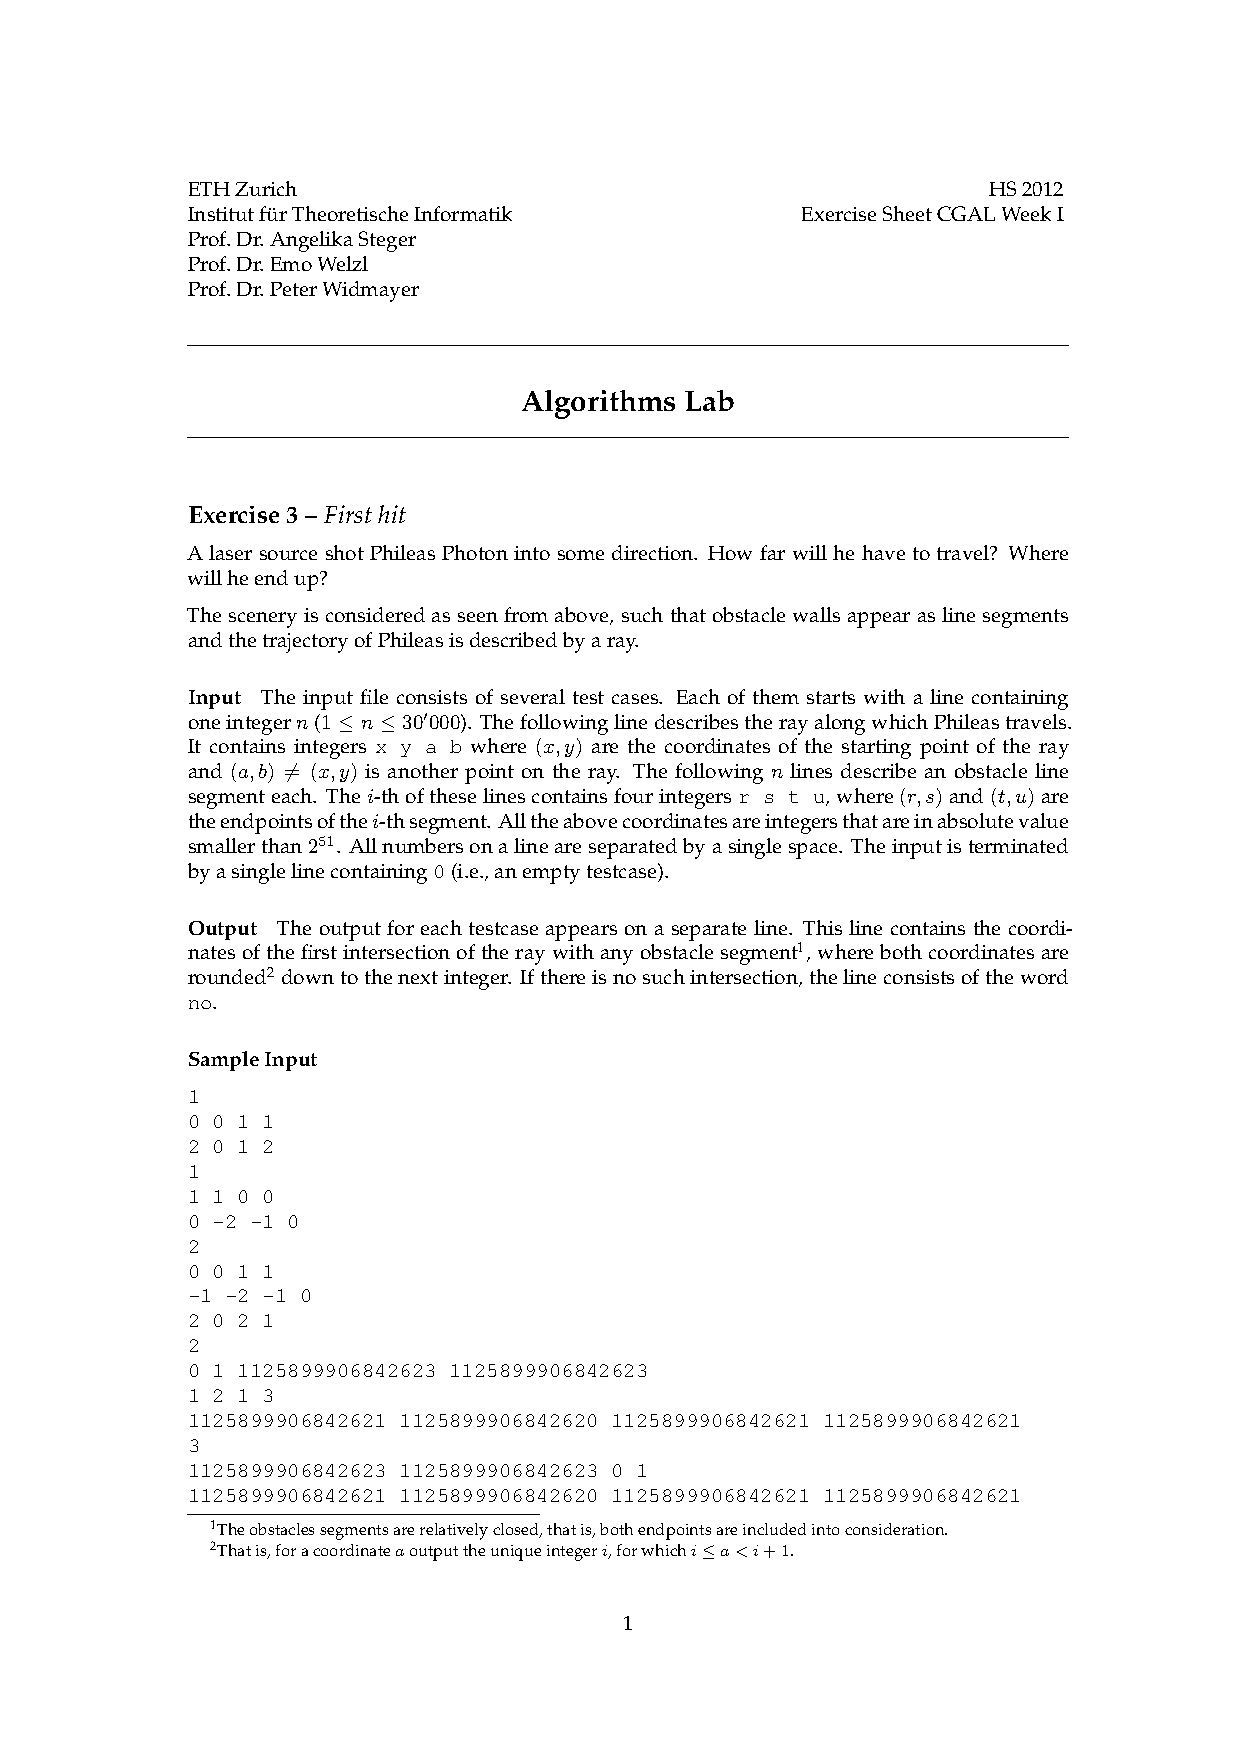
\includepdf{./week_8_cgal/2_first_hit/ex3.pdf}
\lstinputlisting{./week_8_cgal/2_first_hit/first_hit/main.cpp}

\newpage
\part{Week 9 - Proximity Sources}
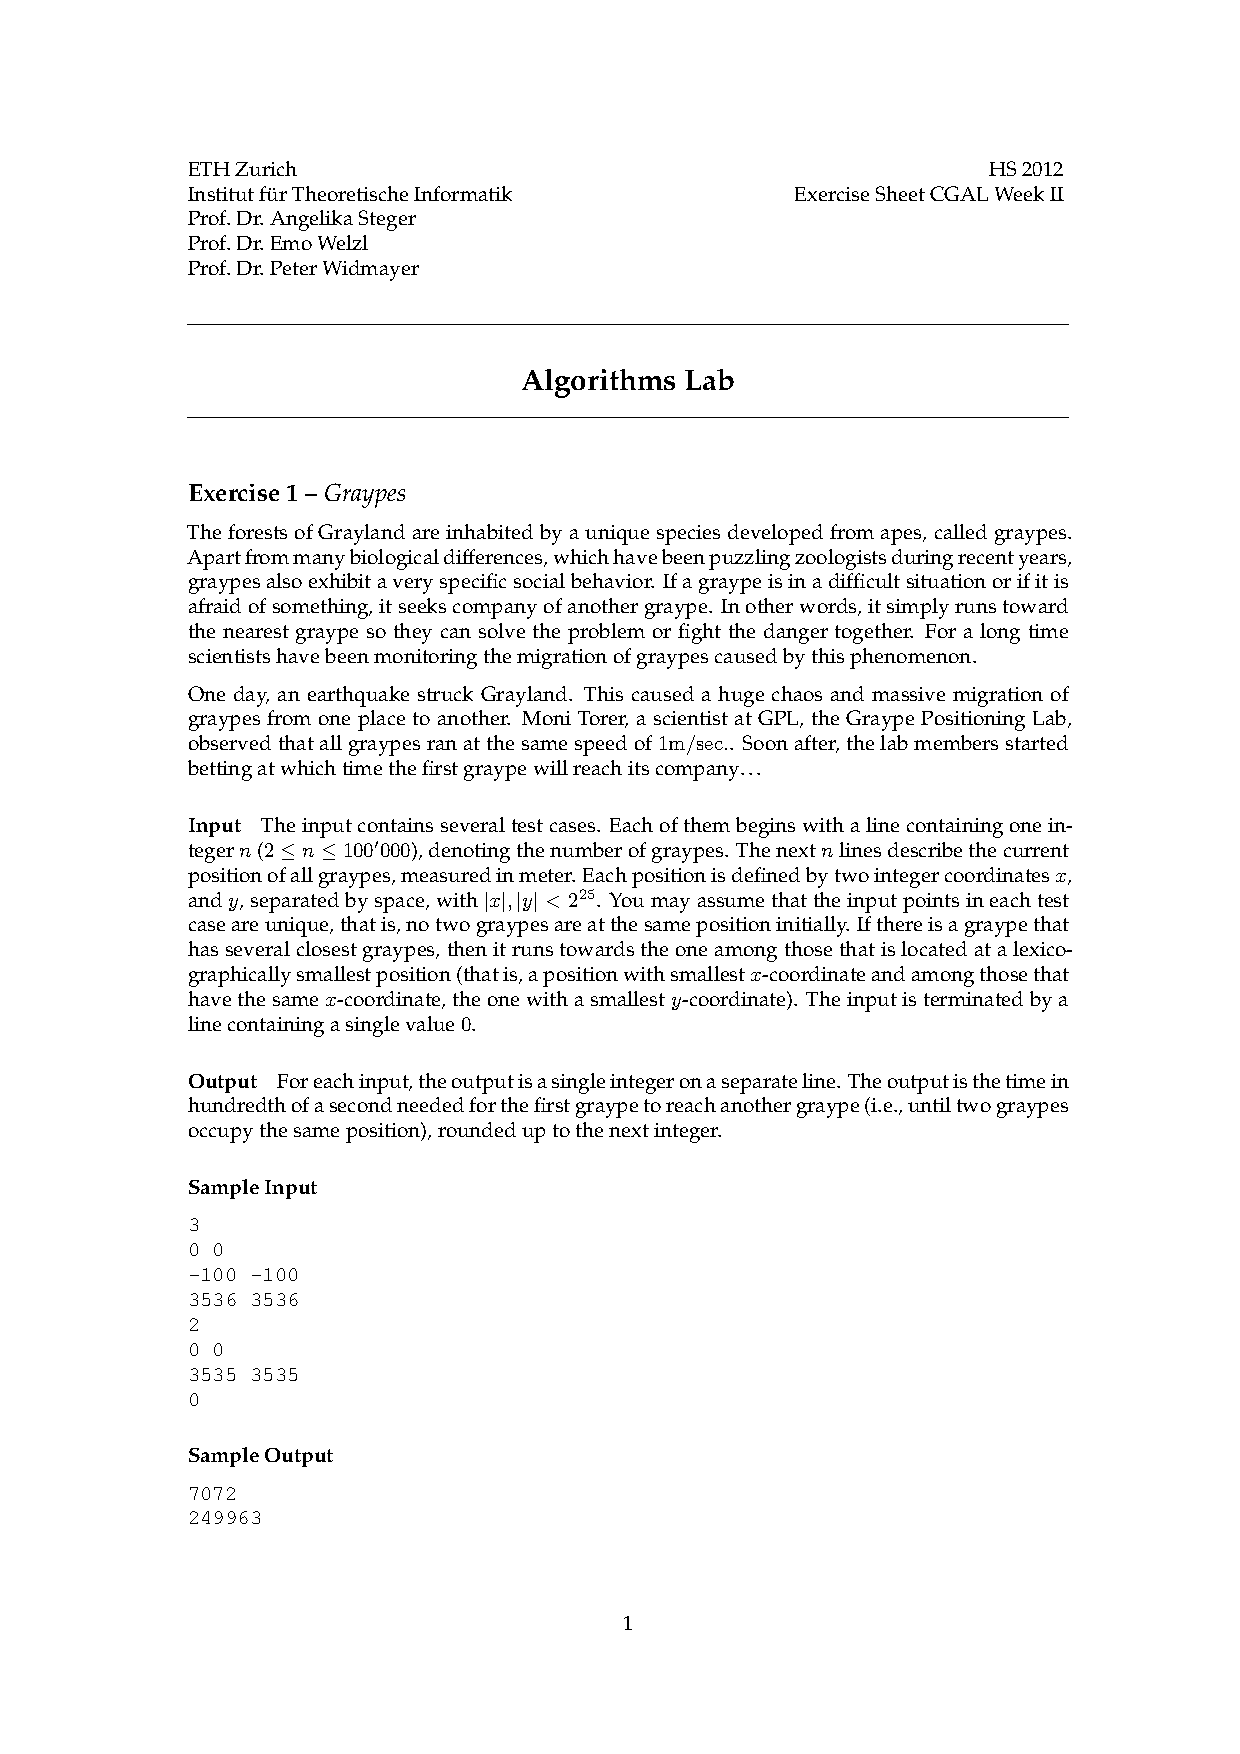
\includepdf{./week_9_proximity_sources/0_graypes/graypes.pdf}
\lstinputlisting{./week_9_proximity_sources/0_graypes/graypes/main.cpp}
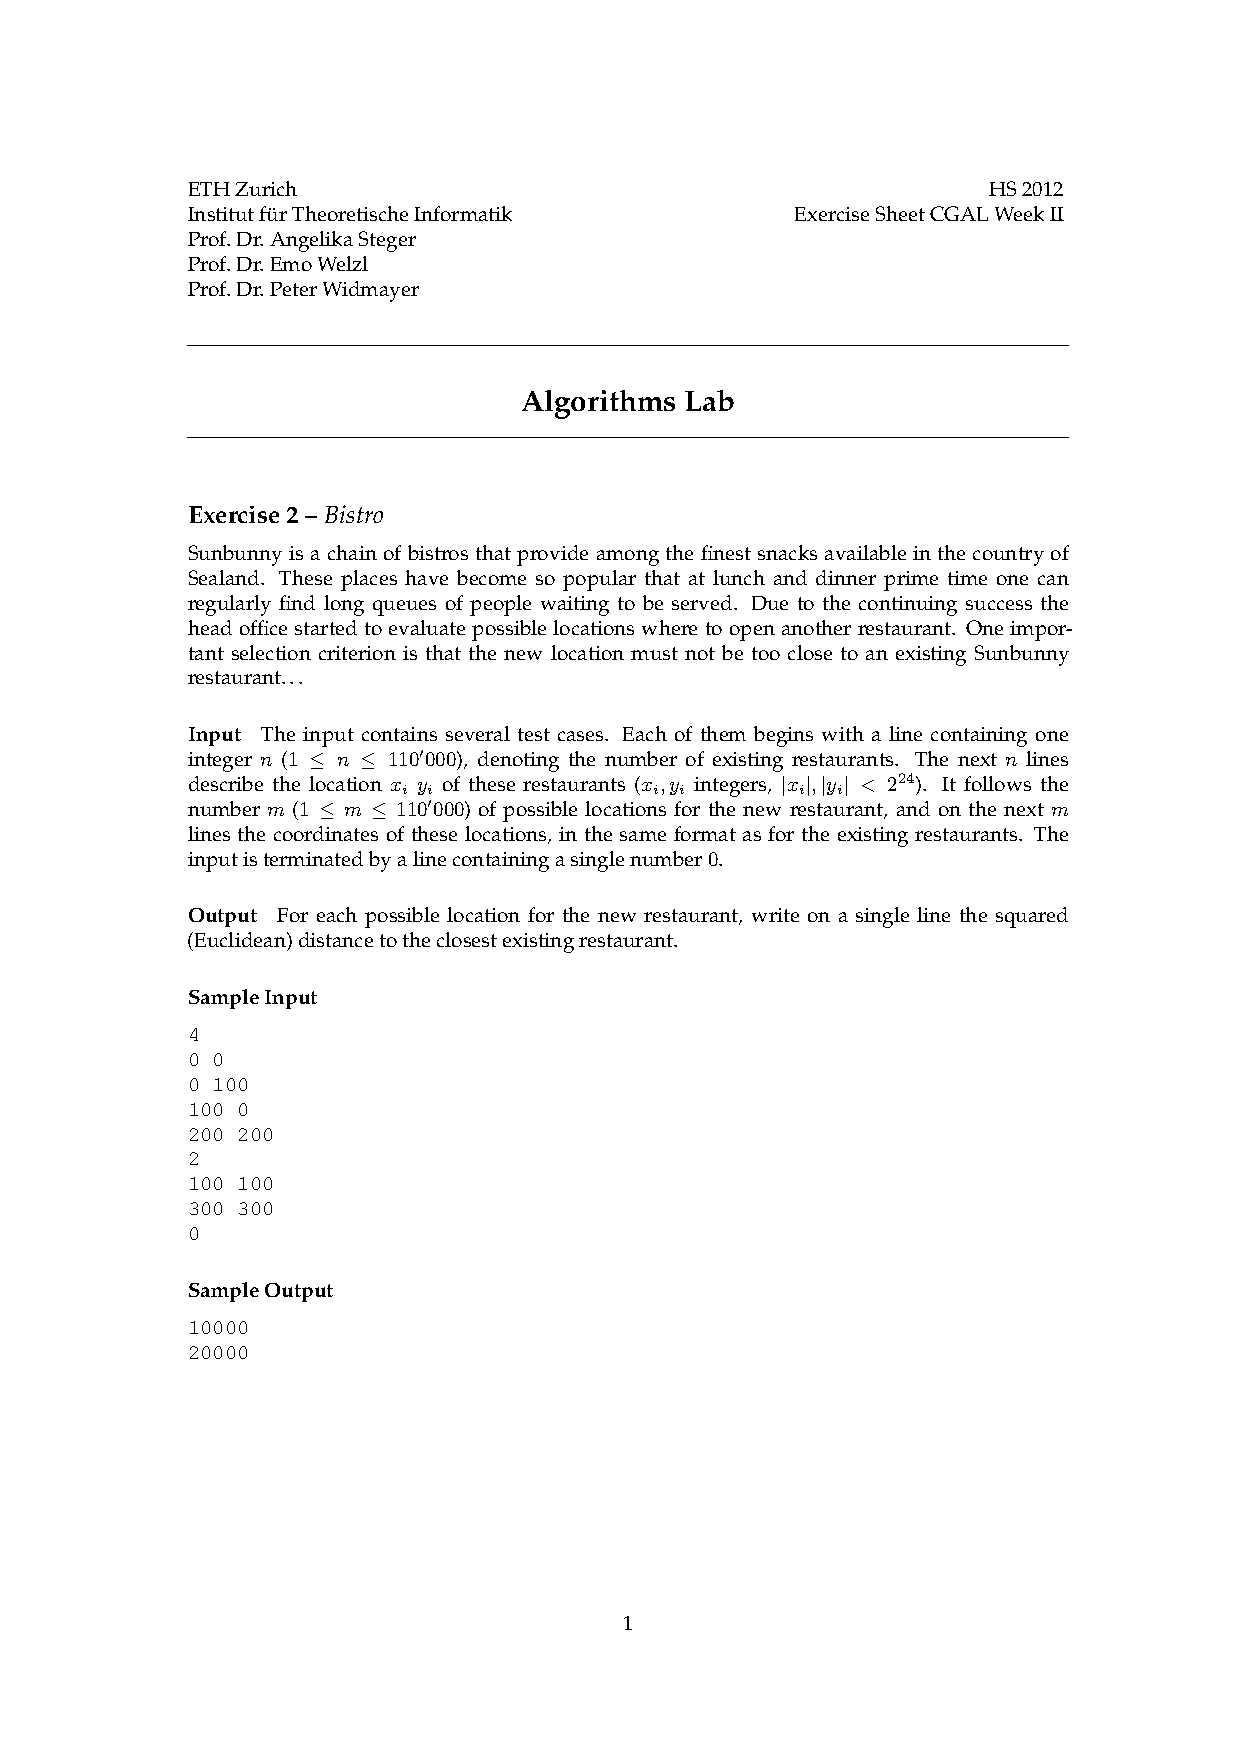
\includepdf{./week_9_proximity_sources/1_bistro/bistro.pdf}
\lstinputlisting{./week_9_proximity_sources/1_bistro/bistro/main.cpp}
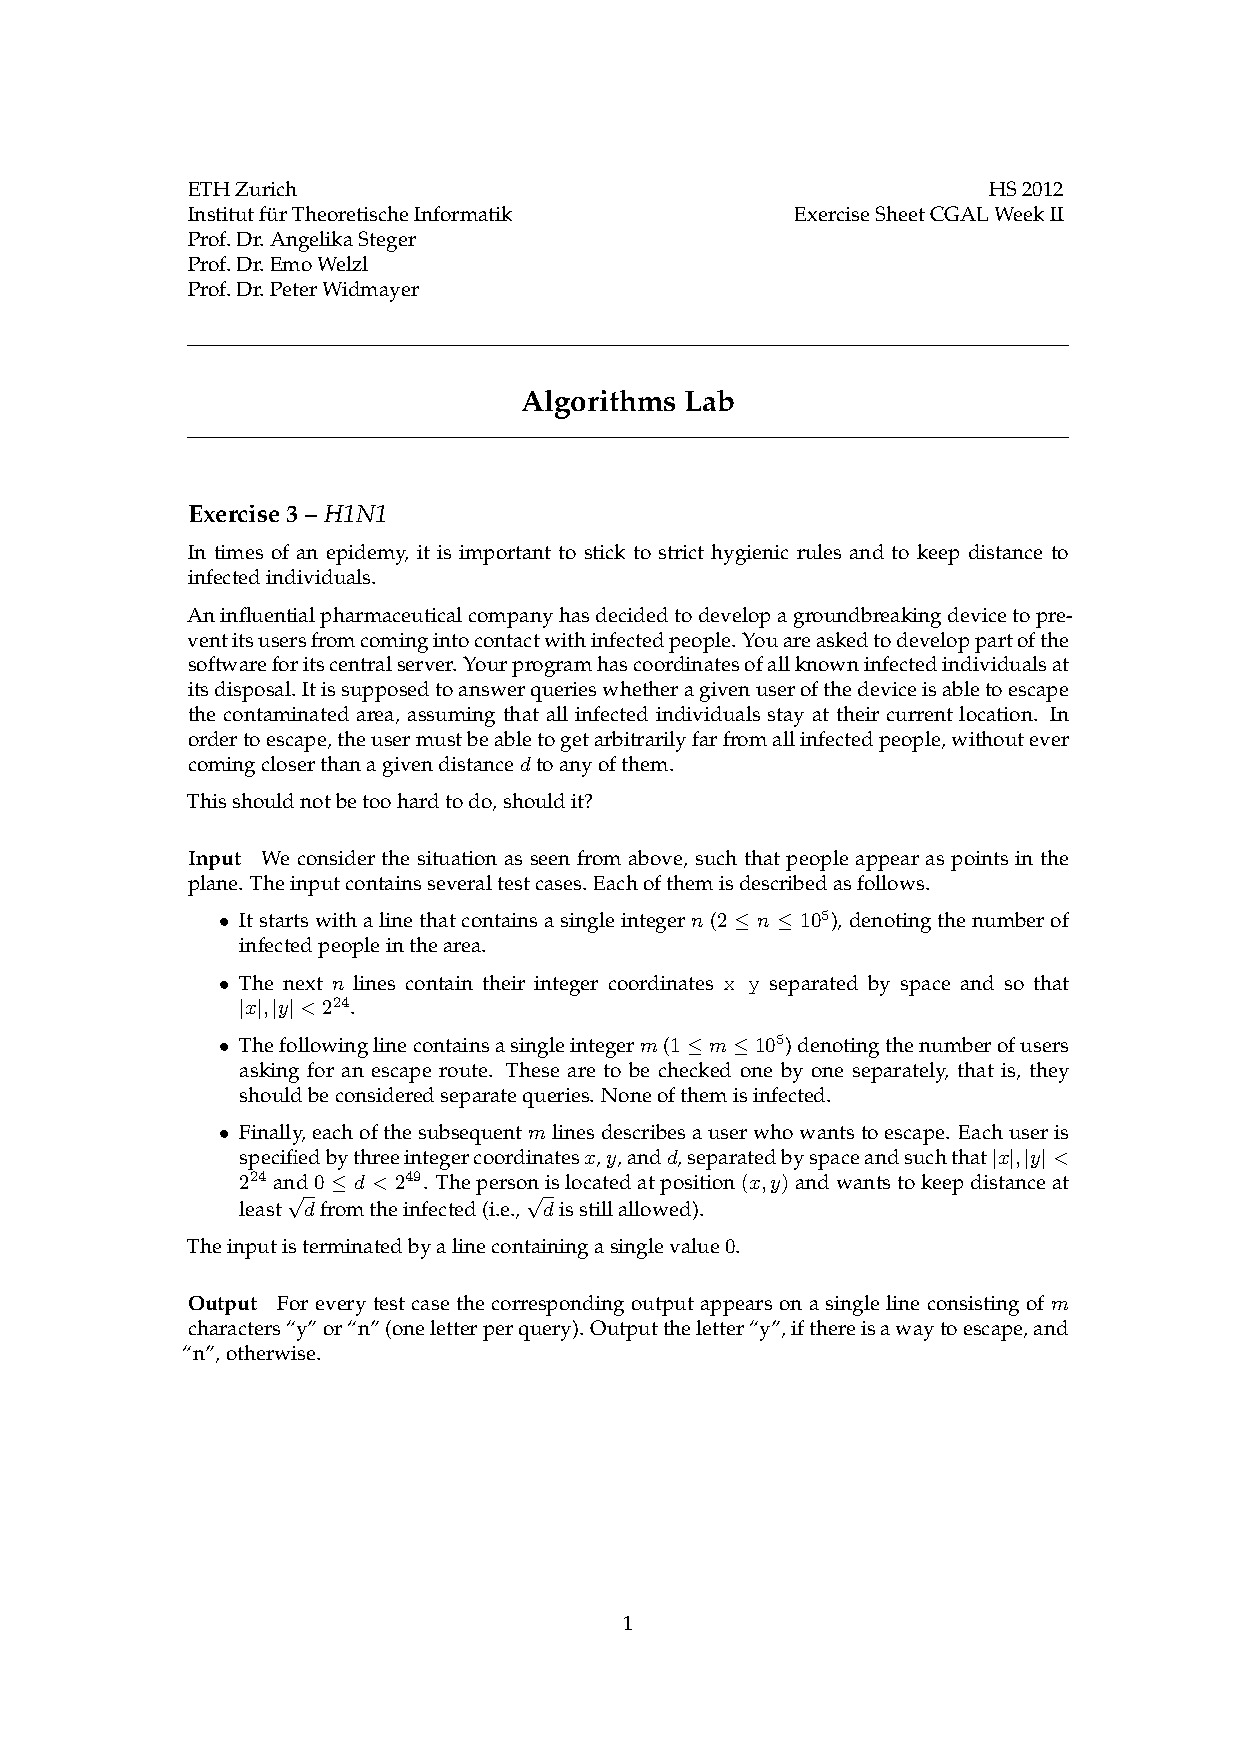
\includepdf{./week_9_proximity_sources/2_h1n1/h1n1.pdf}
\lstinputlisting{./week_9_proximity_sources/2_h1n1/h1n1/main.cpp}
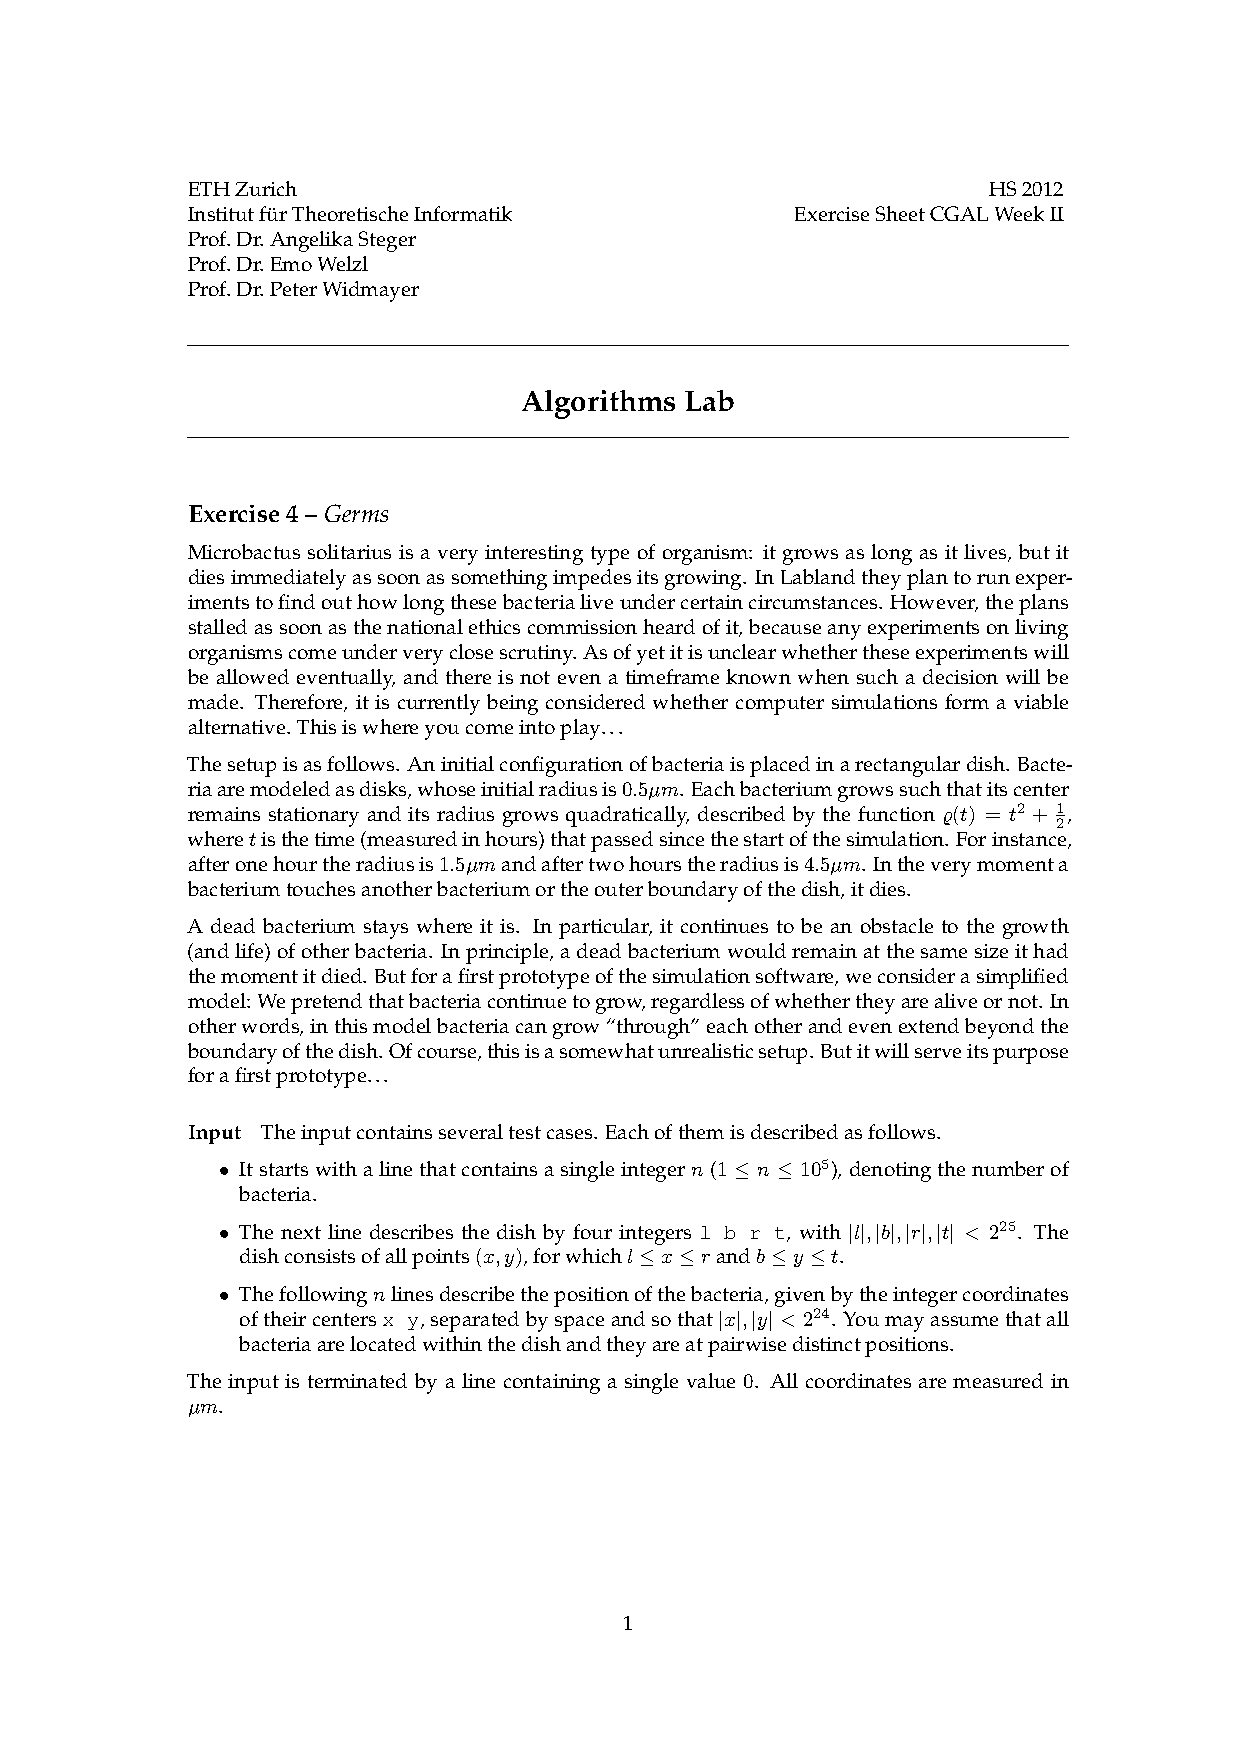
\includepdf{./week_9_proximity_sources/3_germs/germs.pdf}
\lstinputlisting{./week_9_proximity_sources/3_germs/germs/main.cpp}

\newpage
\part{Week 10 - Linear and Quadratic Programming}
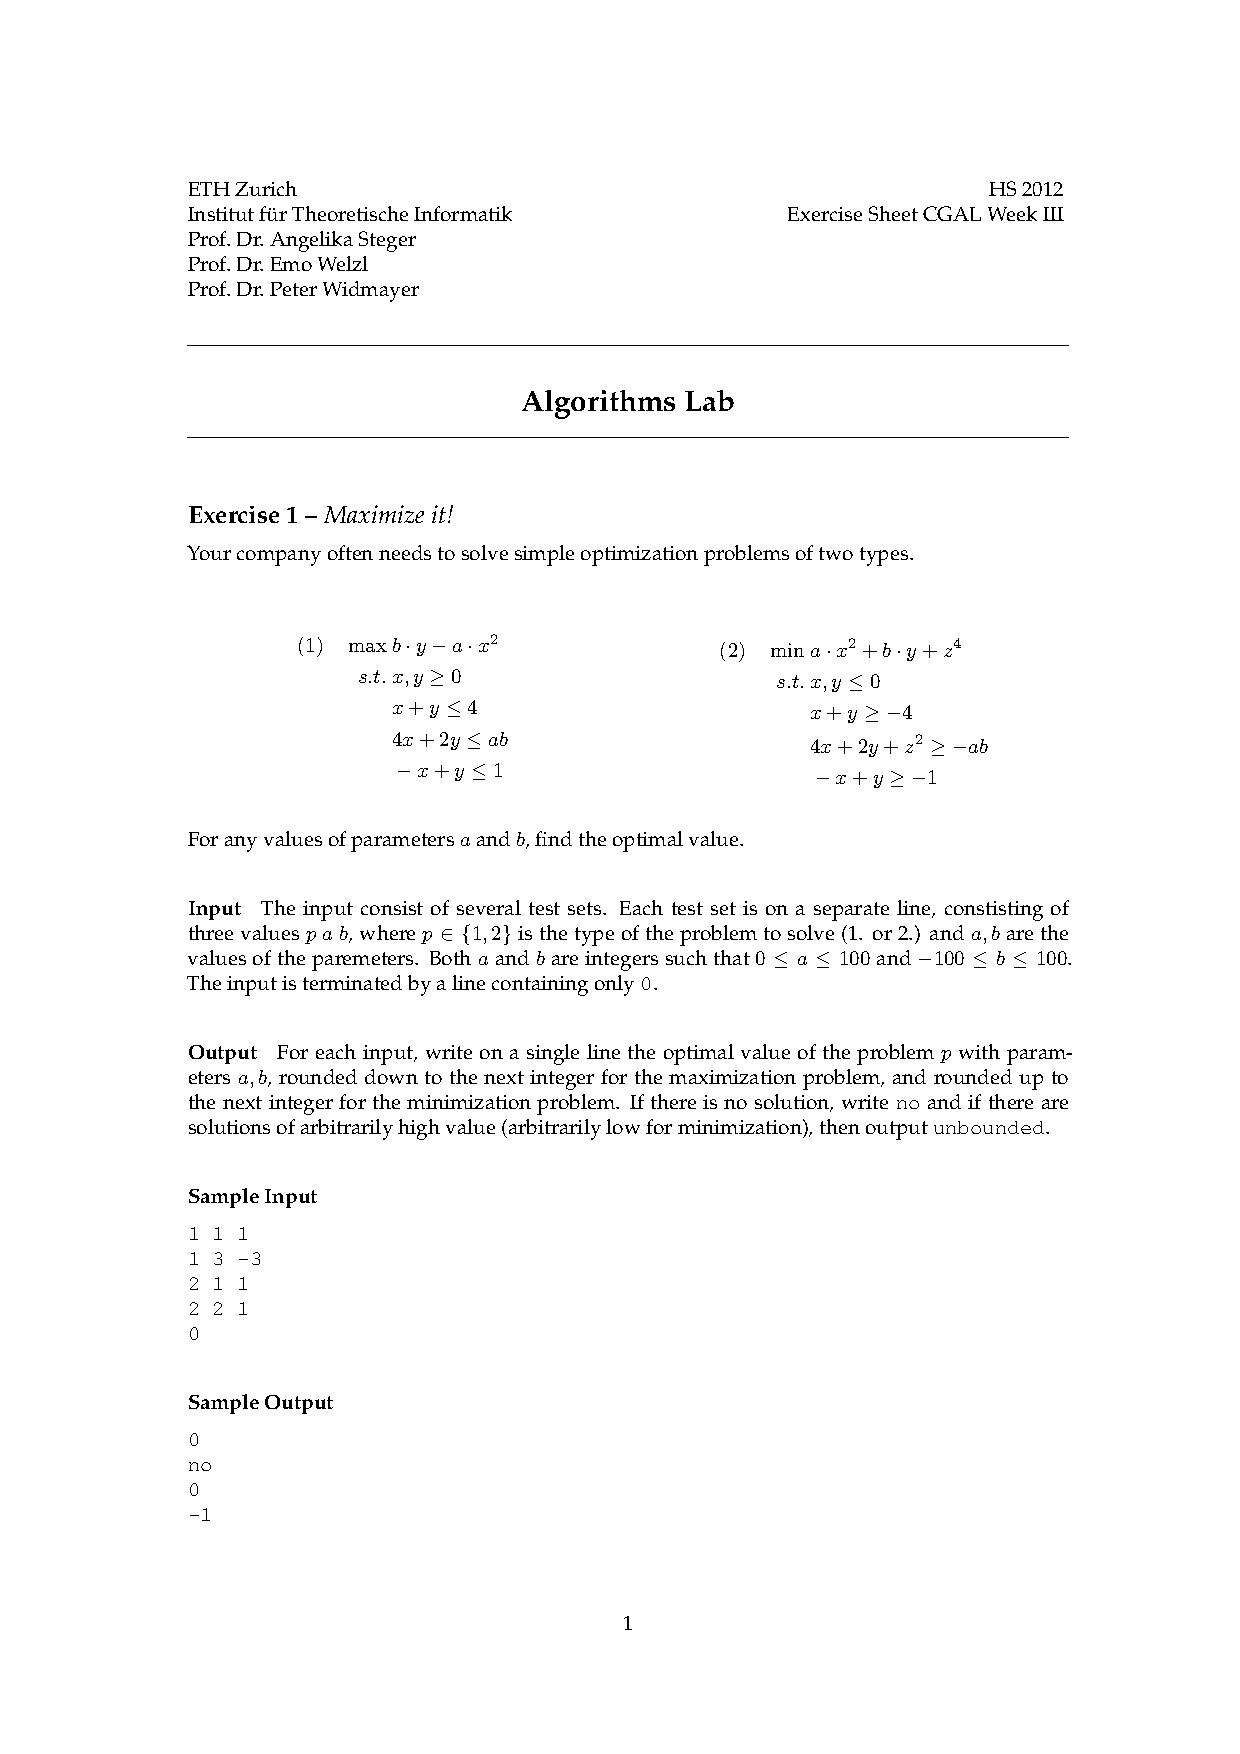
\includepdf{./week_10_linear_and_quadratic_programming/0_maximize/maximizeit.pdf}
\lstinputlisting{./week_10_linear_and_quadratic_programming/0_maximize/maximize/main.cpp}
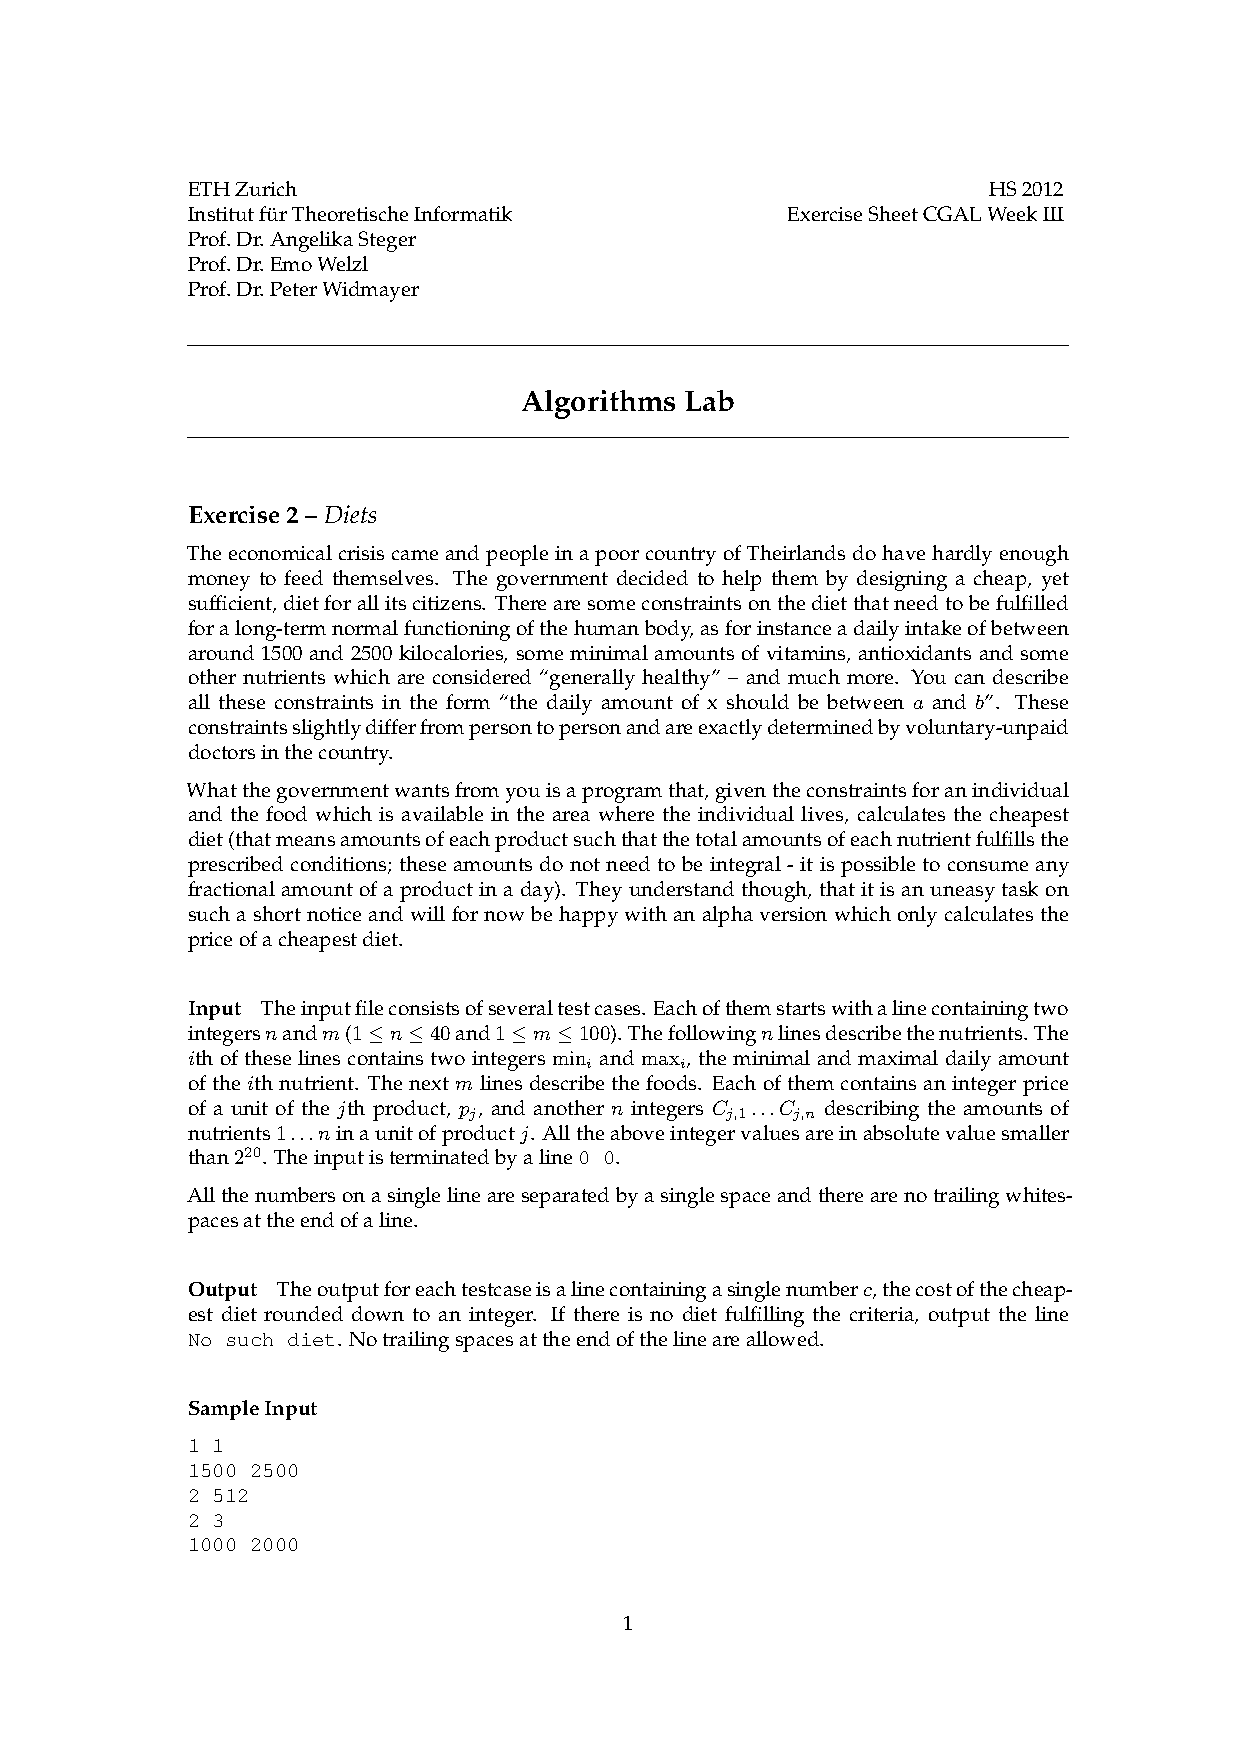
\includepdf{./week_10_linear_and_quadratic_programming/1_diet/diet.pdf}
\lstinputlisting{./week_10_linear_and_quadratic_programming/1_diet/diet/main.cpp}
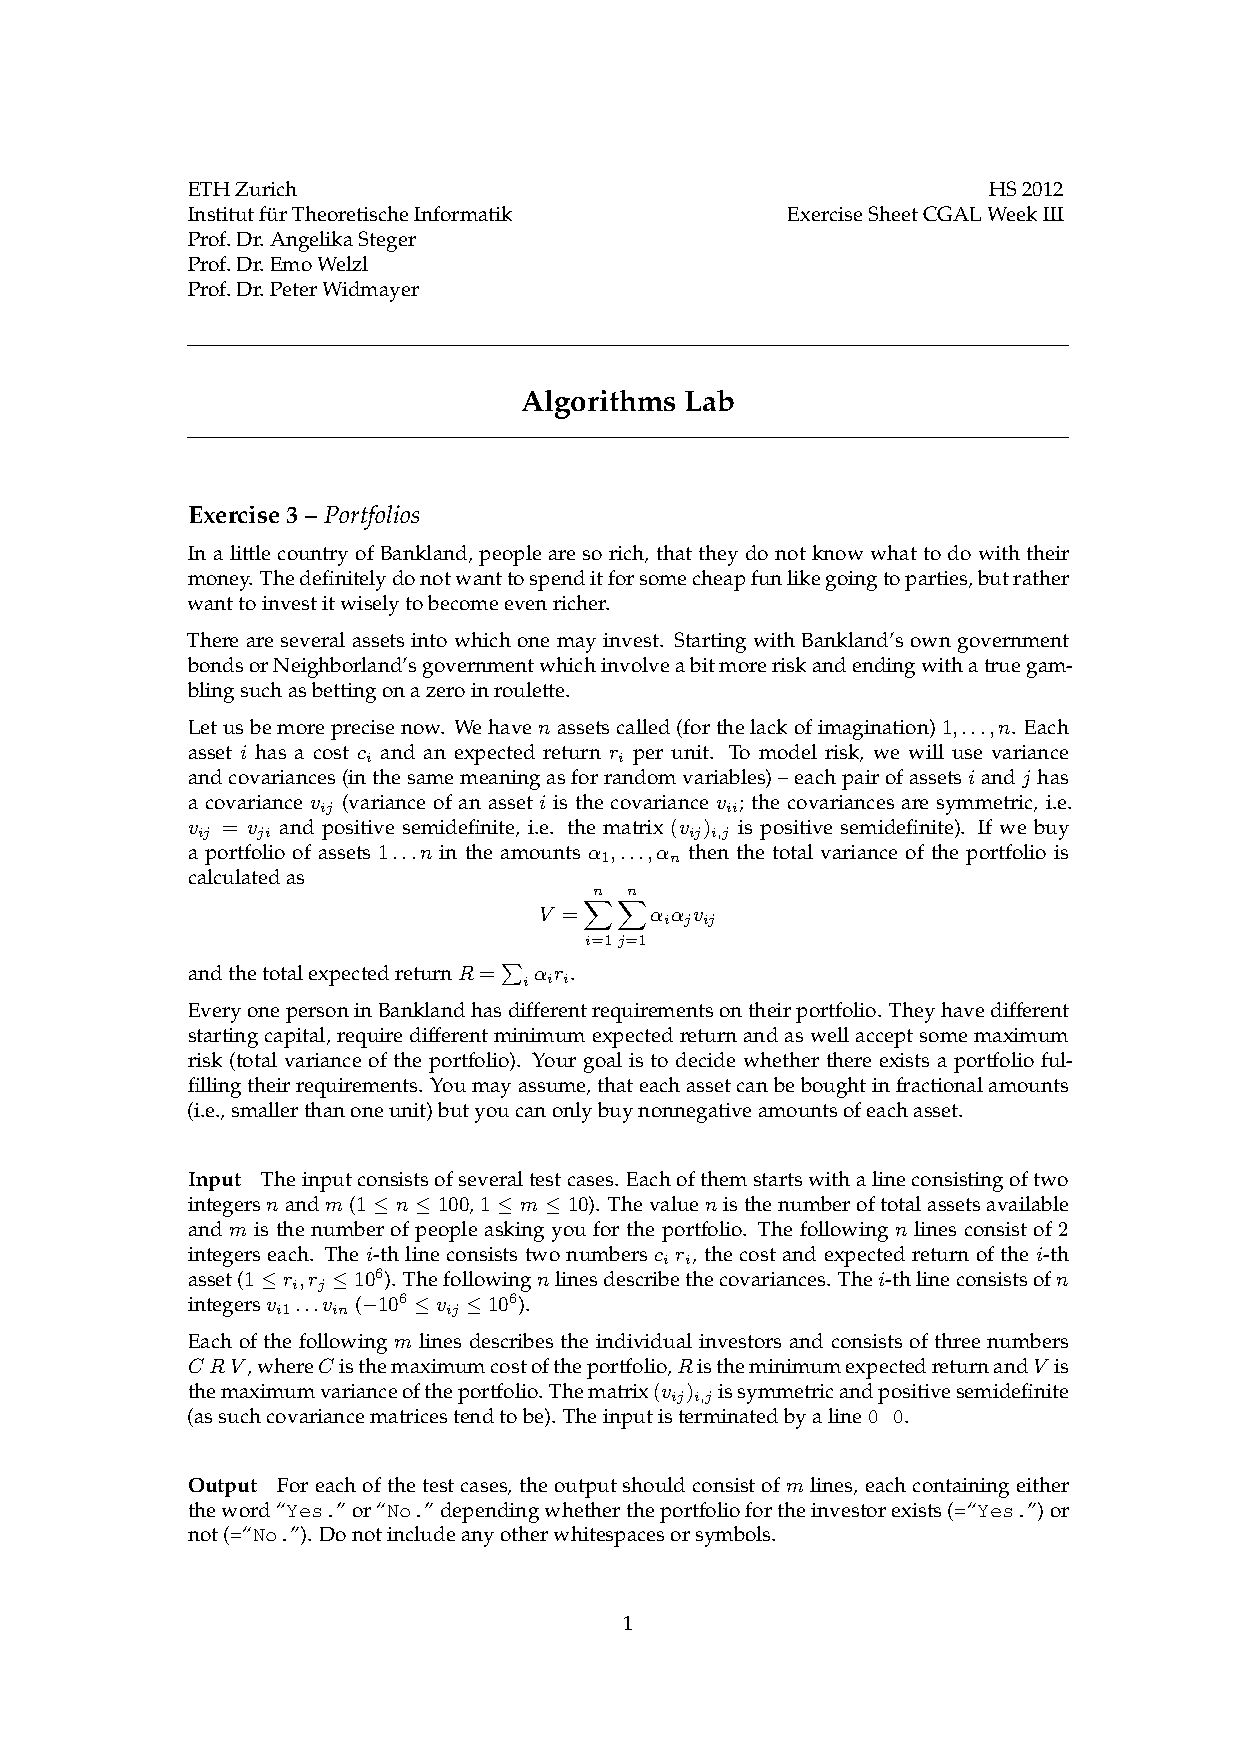
\includepdf{./week_10_linear_and_quadratic_programming/2_portfolios/portfolios.pdf}
\lstinputlisting{./week_10_linear_and_quadratic_programming/2_portfolios/portfolios/main.cpp}
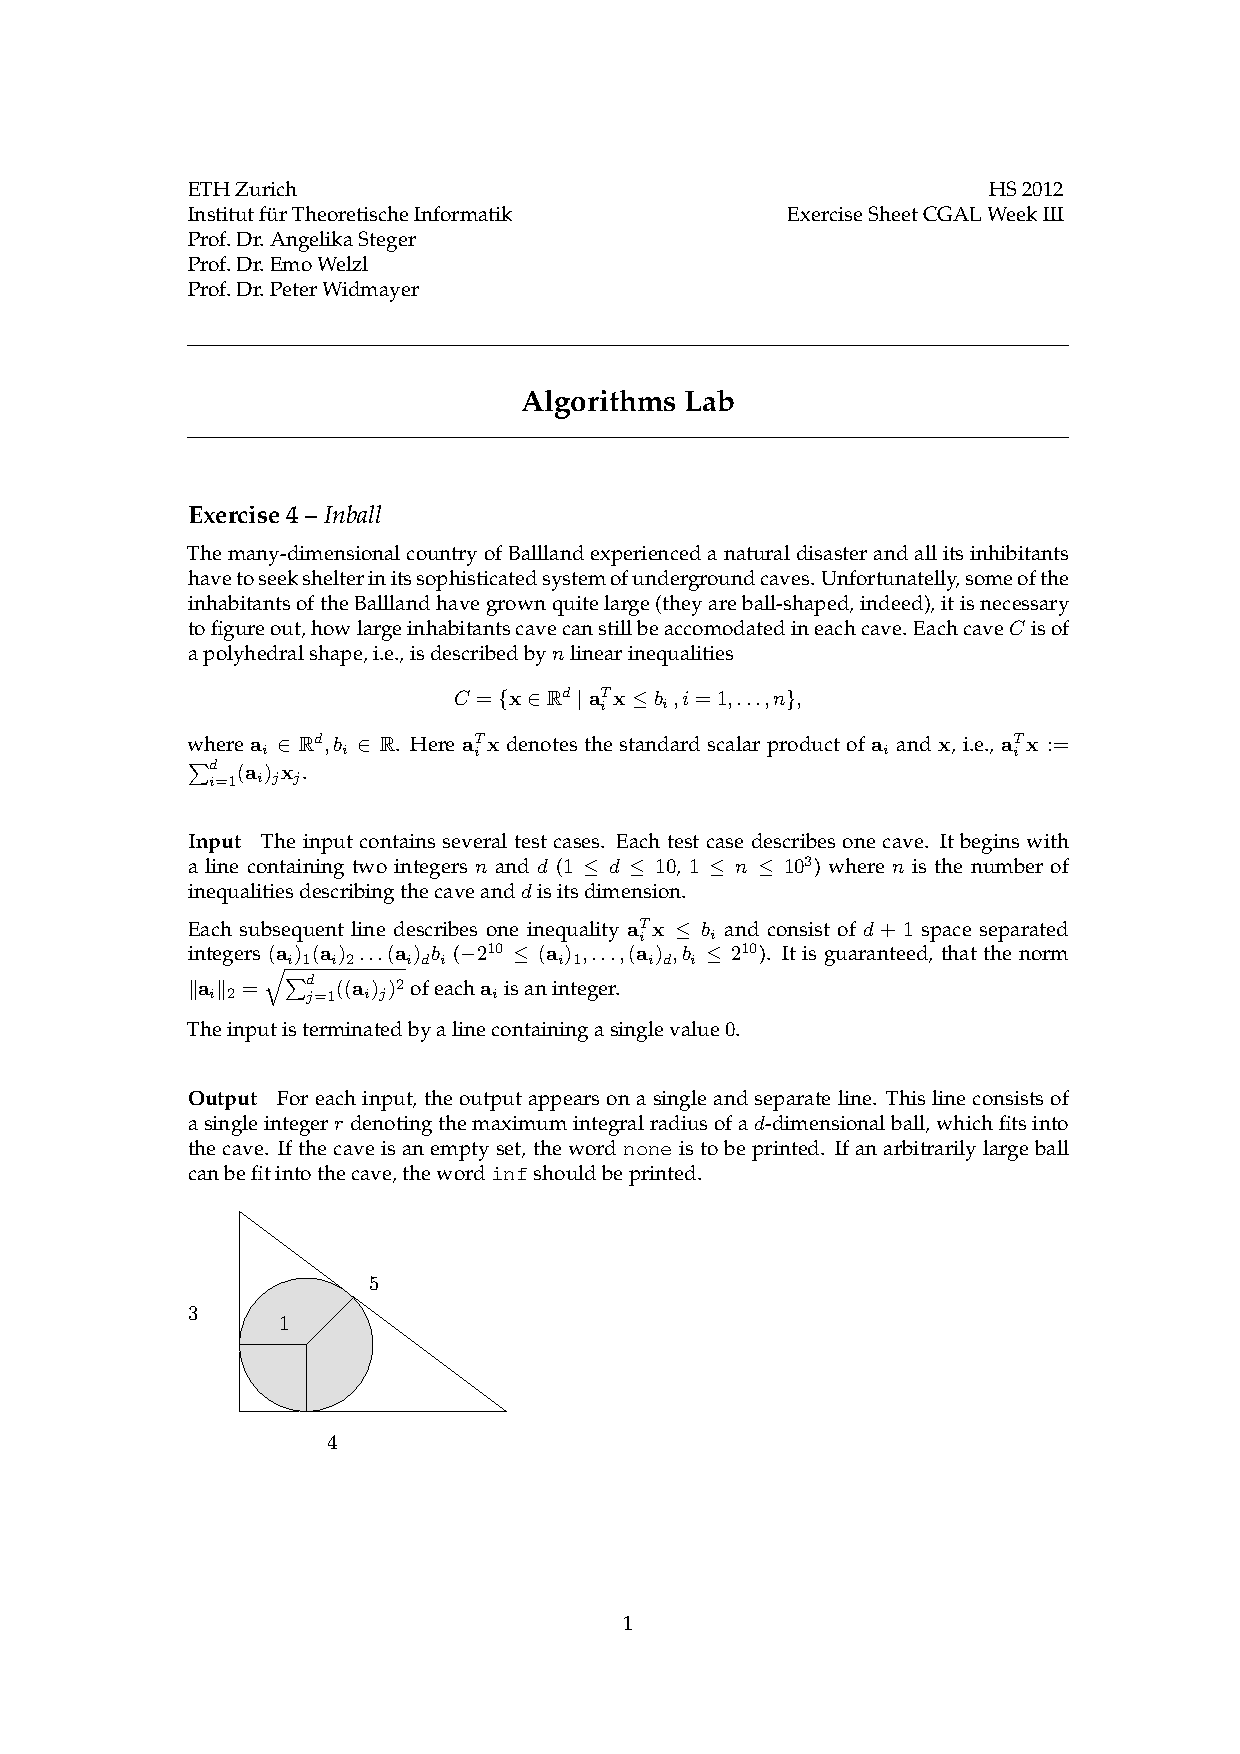
\includepdf{./week_10_linear_and_quadratic_programming/3_inball/inball.pdf}
\lstinputlisting{./week_10_linear_and_quadratic_programming/3_inball/inball/main.cpp}
%\input{01_mass-spring}
%\newpage
%\input{02_constraints}
%\newpage
%\input{03_applied_pdes}
%\newpage
%\input{04_rigid_bodies}
%\newpage
%\input{05_fluids}
\end{document}